\documentclass[review]{elsarticle}

\usepackage{lineno,hyperref}
\modulolinenumbers[5]
\usepackage{soul,color}

\journal{Journal of \LaTeX\ Templates}
\setcitestyle{super,sort&compress}
\bibliographystyle{elsarticle-num}
\usepackage{array}
\newcolumntype{C}[1]{>{\centering\let\newline\\\arraybackslash\hspace{0pt}}m{#1}}
\newcolumntype{P}[1]{>{\centering\arraybackslash}p{#1}}
\newcolumntype{M}[1]{>{\centering\arraybackslash}m{#1}}

\usepackage{footnote}
\usepackage[symbol]{footmisc}
\makesavenoteenv{tabular}
\makesavenoteenv{table}
\usepackage{booktabs} % For formal tables
\usepackage[ruled]{algorithm2e} % For algorithms
\usepackage{txfonts}
\usepackage{graphicx}
\usepackage{subcaption}
%\usepackage{amsmath}
\usepackage{lmodern}
\usepackage{multirow}

\begin{document}
\begin{frontmatter}
	
	\title{Finger Texture Biometric Characteristic: A Survey}

\author{Raid R. O. Al-Nima $^{1,2}$, Tingting Han$^{2}$, Taolue Chen$^{2}$, Satnam Dlay$^{3}$, and Jonathon Chambers$^{4}$}
\address{$^{1}$ Technical Engineering College of Mosul, \\Northern Technical University, Mosul, Iraq\\
raidrafi1@gmail.com}
\address{$^{2}$ Department of Computer Science and Information Systems, \\Birkbeck, University of London, London, UK\\
tingting@dcs.bbk.ac.uk, and t.chen@dcs.bbk.ac.uk}
\address{$^{3}$ School of Engineering, Newcastle University, \\Newcastle upon Tyne, UK\\
satnam.dlay@ncl.ac.uk}
\address{$^{4}$ Department of Engineering, University of Leicester \\Leicester, UK\\
Jonathon.Chambers@le.ac.uk}

\begin{abstract}
	Rich characteristics can be observed in each single finger. First of all, they hold the most widely used biometric - the fingerprint. Other biometrics embedded in a finger are the Finger Geometry (FG), Finger Veins (FV), Finger Outer Knuckle (FOK), Finger Inner Knuckle (FIK) and Finger Nail-bed (FN), etc. In recent years, the Finger Texture (FT) has attracted considerable attention as a biometric characteristic. They can provide efficient human recognition performance, because they have different human-specific features of apparent lines, wrinkles and ridges distributed along the inner surface of all fingers. Also, their pattern structures are reliable, unique and remain stable throughout a human's life. Efficient biometric systems can be established based on FTs only. In this paper, a comprehensive survey of the relevant FT studies is presented. We also summarise the main drawbacks and obstacles of employing the FT as a biometric characteristic, followed by useful suggestions to further improve the work on FT. 
\end{abstract}

\begin{keyword}
	\texttt{Finger Texture, Finger Inner Surface, Biometrics, Pattern Recognition}
\end{keyword}

\end{frontmatter}

\linenumbers

\section{Introduction}
	\hl{Biometric recognition can be considered as one of the most important components of a large number of security systems. Examples of some technologies which can employ a biometric characteristic to authenticate the automatic access are mobile phones, laptops, private computers and Automated Teller Machines (ATMs)} \cite{Jain2004AnIntroduction}\hl{. Efficient biometric systems that are using more than one biometric characteristic can be found specifically in some very high security buildings. Without biometric recognition such products and buildings may be attacked by unlicensed or unauthorized people.}	In general, biometric characteristics can be divided into two main classes: soft and hard \cite{jaswal2016knuckle}. The soft biometrics represent the traits that are used in describing people such as weight, height, hair color, ethnicity, age, gender, etc. This type of biometrics has been utilized in categorizing individuals, exploited in surveillance investigations and applied to other biometric characteristics \cite{dantcheva2016else}. Moreover, the hard biometric traits are divided into two types as follows:
	\begin{enumerate}
		\item Physiological biometrics: this type of biometric refers to the physiological traits within the human body such as the fingerprint, iris print and palmprint. 
		\item Behavioural biometrics: this type of biometric refers to the behavioural traits of the individual style such as the signature, keystroke and voice. 
	\end{enumerate}

	The physiological biometrics are usually more accurate and reliable, whereas the behavioural biometrics may be affected by the emotional feelings such as sickness or tension \cite{matyavs2000biometric}. A number of specifications are required for each physiological or behavioural trait in order to be considered as a biometric characteristic. These specifications are highlighted as follows \cite{Jain2004AnIntroduction}:
	\begin{itemize}
		\item Stability: the biometric patterns have to be stable and permanent.
		\item Uniqueness: the features of the trait must be unique and vary between any two individuals.
		\item Collectability: this means that the collected biometric features should be valuable and measurable.
		\item Popularity: the trait should be popular or non-exclusive for certain individual(s). 
	\end{itemize}

	In addition, the biometric systems are highly preferable to have the following factors \cite{Jain2004AnIntroduction}:
	\begin{itemize}
		\item Suitability: this refers to the acceptability as a user-friendly biometric system. 
		\item Implementation: the biometric system has to be highly applicable and trustworthy.
		\item Circumvention: the biometric system should be difficult to avoid by fraudsters.
	\end{itemize}

	Therefore, it is necessary to consider the seven factors above to establish a robust biometric system. 
	
	Many people think that only part of finger that can be considered in biometric systems is the fingerprint. However, each single finger holds many biometric characteristics. Some finger biometric characteristics only appeared approximately one decade ago. It is important to present these patterns and explain the advantages and disadvantages of using each one of them. It is worth highlighting that FT has superior specifications over other finger biometrics. Table \ref{Table:Physiological_biometrics} shows the various physiological finger characteristics.
	
%	\begin{figure}[!h]
%		\centering
%		\includegraphics[page=1,scale=.55,trim=4cm 5cm 4cm 5cm,clip]{Various_Finger_Characteristics1.pdf}
%		\caption{Various Finger Characteristics}
%		\label{fig:Various_Finger_Characteristics}
%	\end{figure}
%Their pattern structures remain stable throughout a human's life. \\
	The inner surface of the finger has recently shown considerable investigations. It has similar features as can be observed in the palm surface. It includes various patterns of ridges, visible lines and skin wrinkles. In general, the ridges require higher resolution images than the lines and wrinkles. So, the visible patterns of the flexion lines and wrinkles have simple and effective features \cite{li2004personal}. The main features of the inner finger surface are expressed in Fig. \ref{fig:FT2}. In general, the FT is positioned in the inner surface of any finger between the upper phalanx (below the fingerprint) and the lower knuckle (the base of the finger). Its patterns are unique and reliable to be considered as a biometric characteristic. \hl{The FTs can be found on the inner surface of five fingers: the four fingers or main fingers (little, ring, middle and index), and the thumb.} Fig. \ref{fig:FTs_locations} shows the main locations of FTs.


	\begin{table}[h]
	\centering
	\caption{\hl{Different physiological characteristics that can be found in each single finger}}
	\label{Table:Physiological_biometrics}
	\scalebox{0.7}{\begin{tabular}{|C{3.7cm}|C{3.7cm}|c|} \hline
			\textbf{Physiological Finger Biometrics} & \textbf{Demonstrated Images} & \textbf{Descriptions}\\ \hline
			\textbf{Fingerprint} &  \begin{minipage}{0.75\hsize}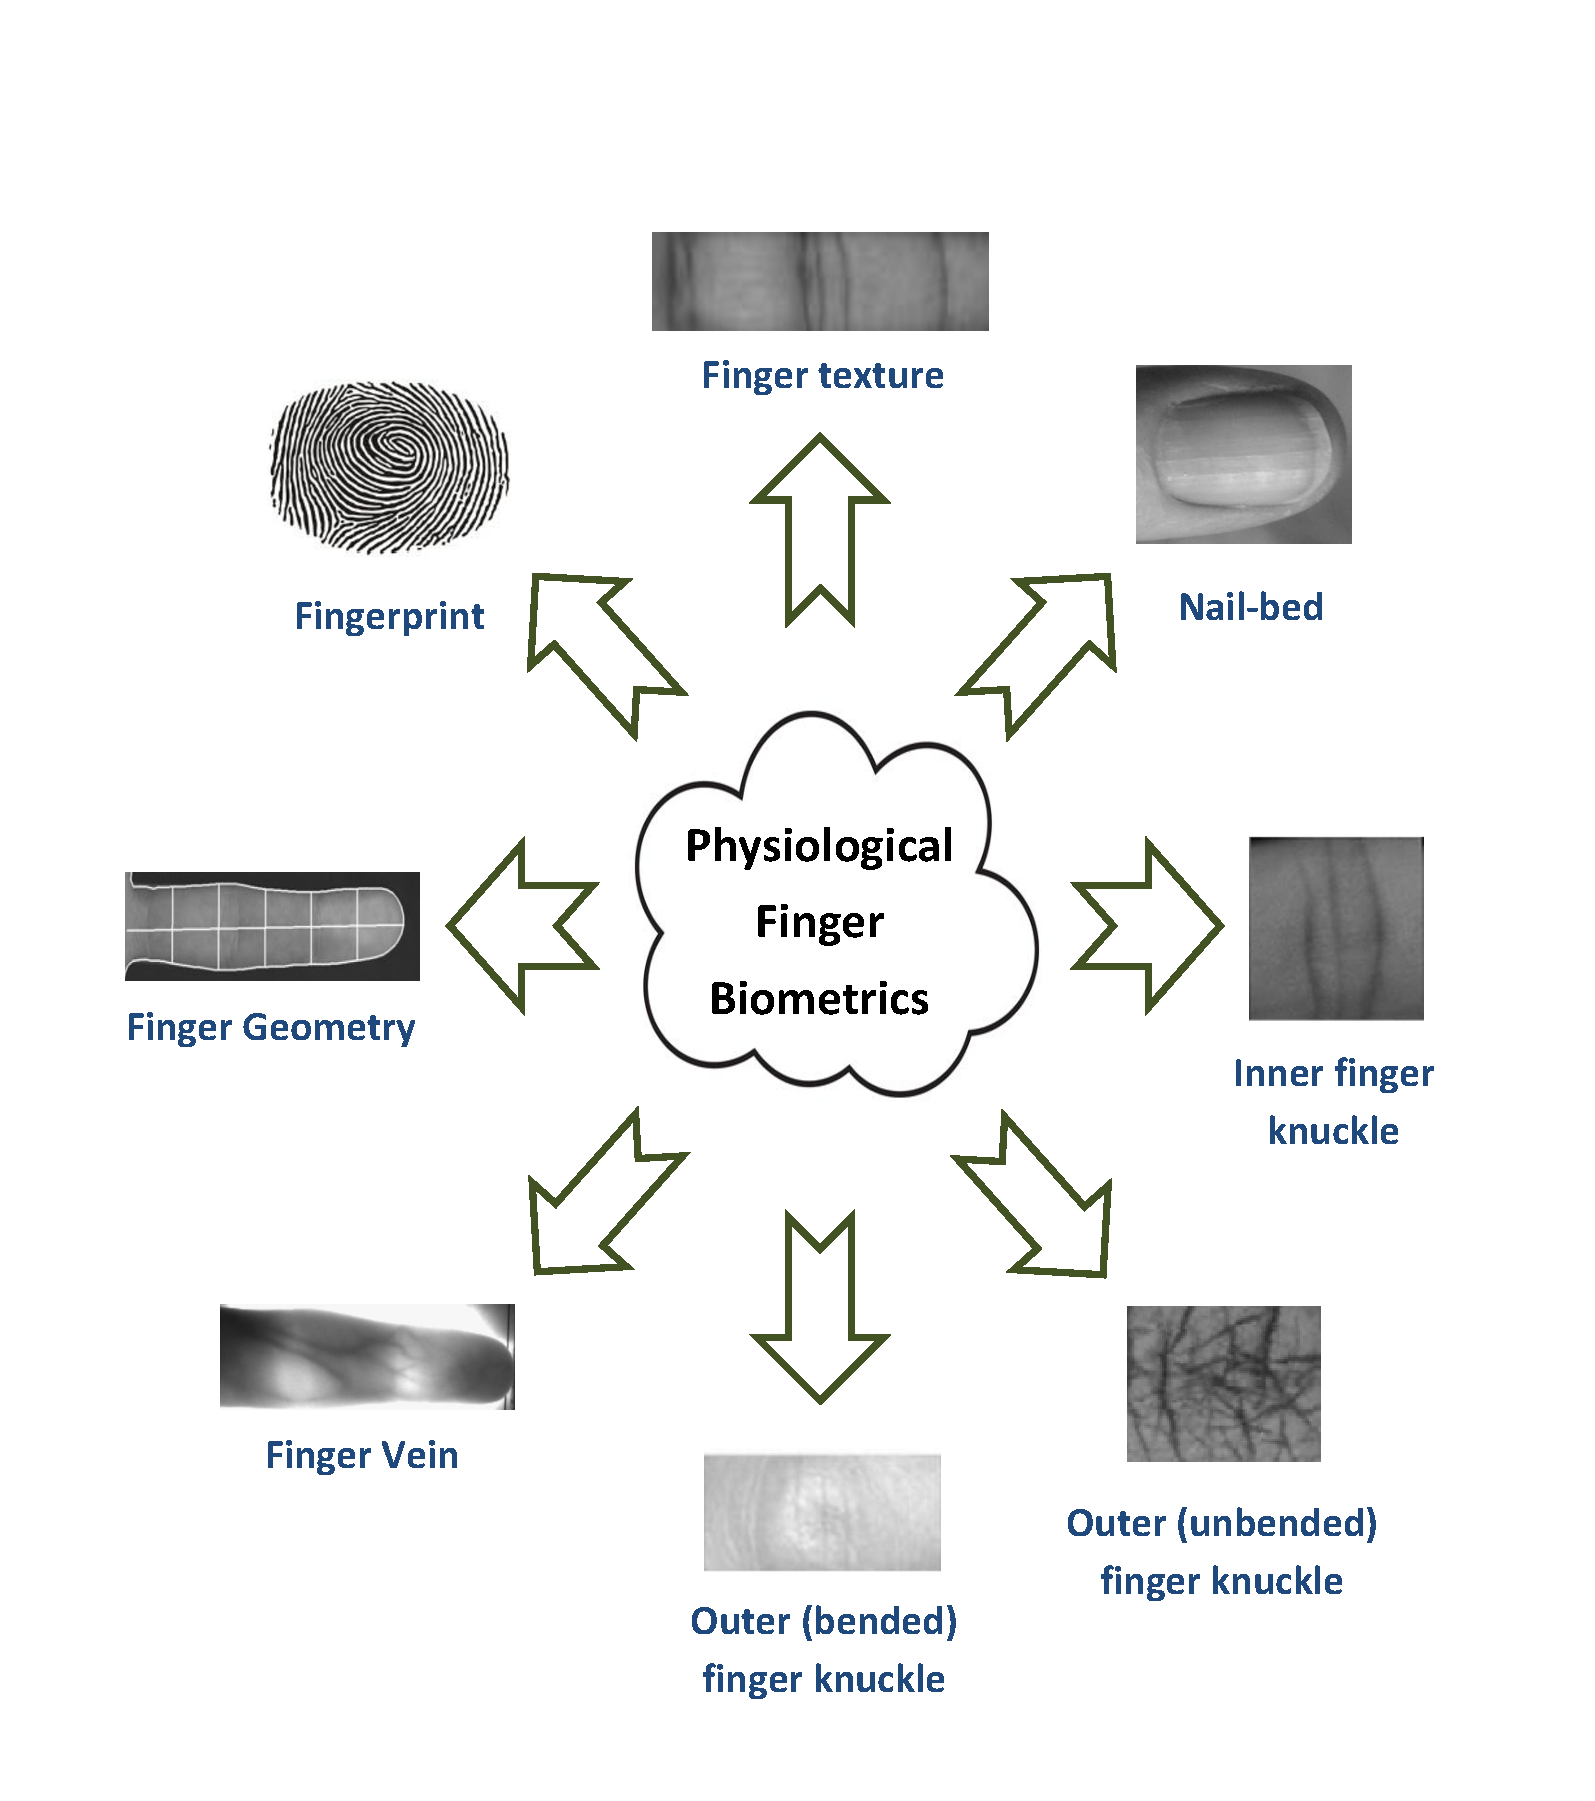
\includegraphics[page=1,scale=.45,trim=4cm 20.8cm 17cm 6cm,clip]{Finger_biometrics.pdf}\end{minipage} & Ridges of a finger tip \\ \hline
			\textbf{Finger Geometry} & \begin{minipage}{0.75\hsize}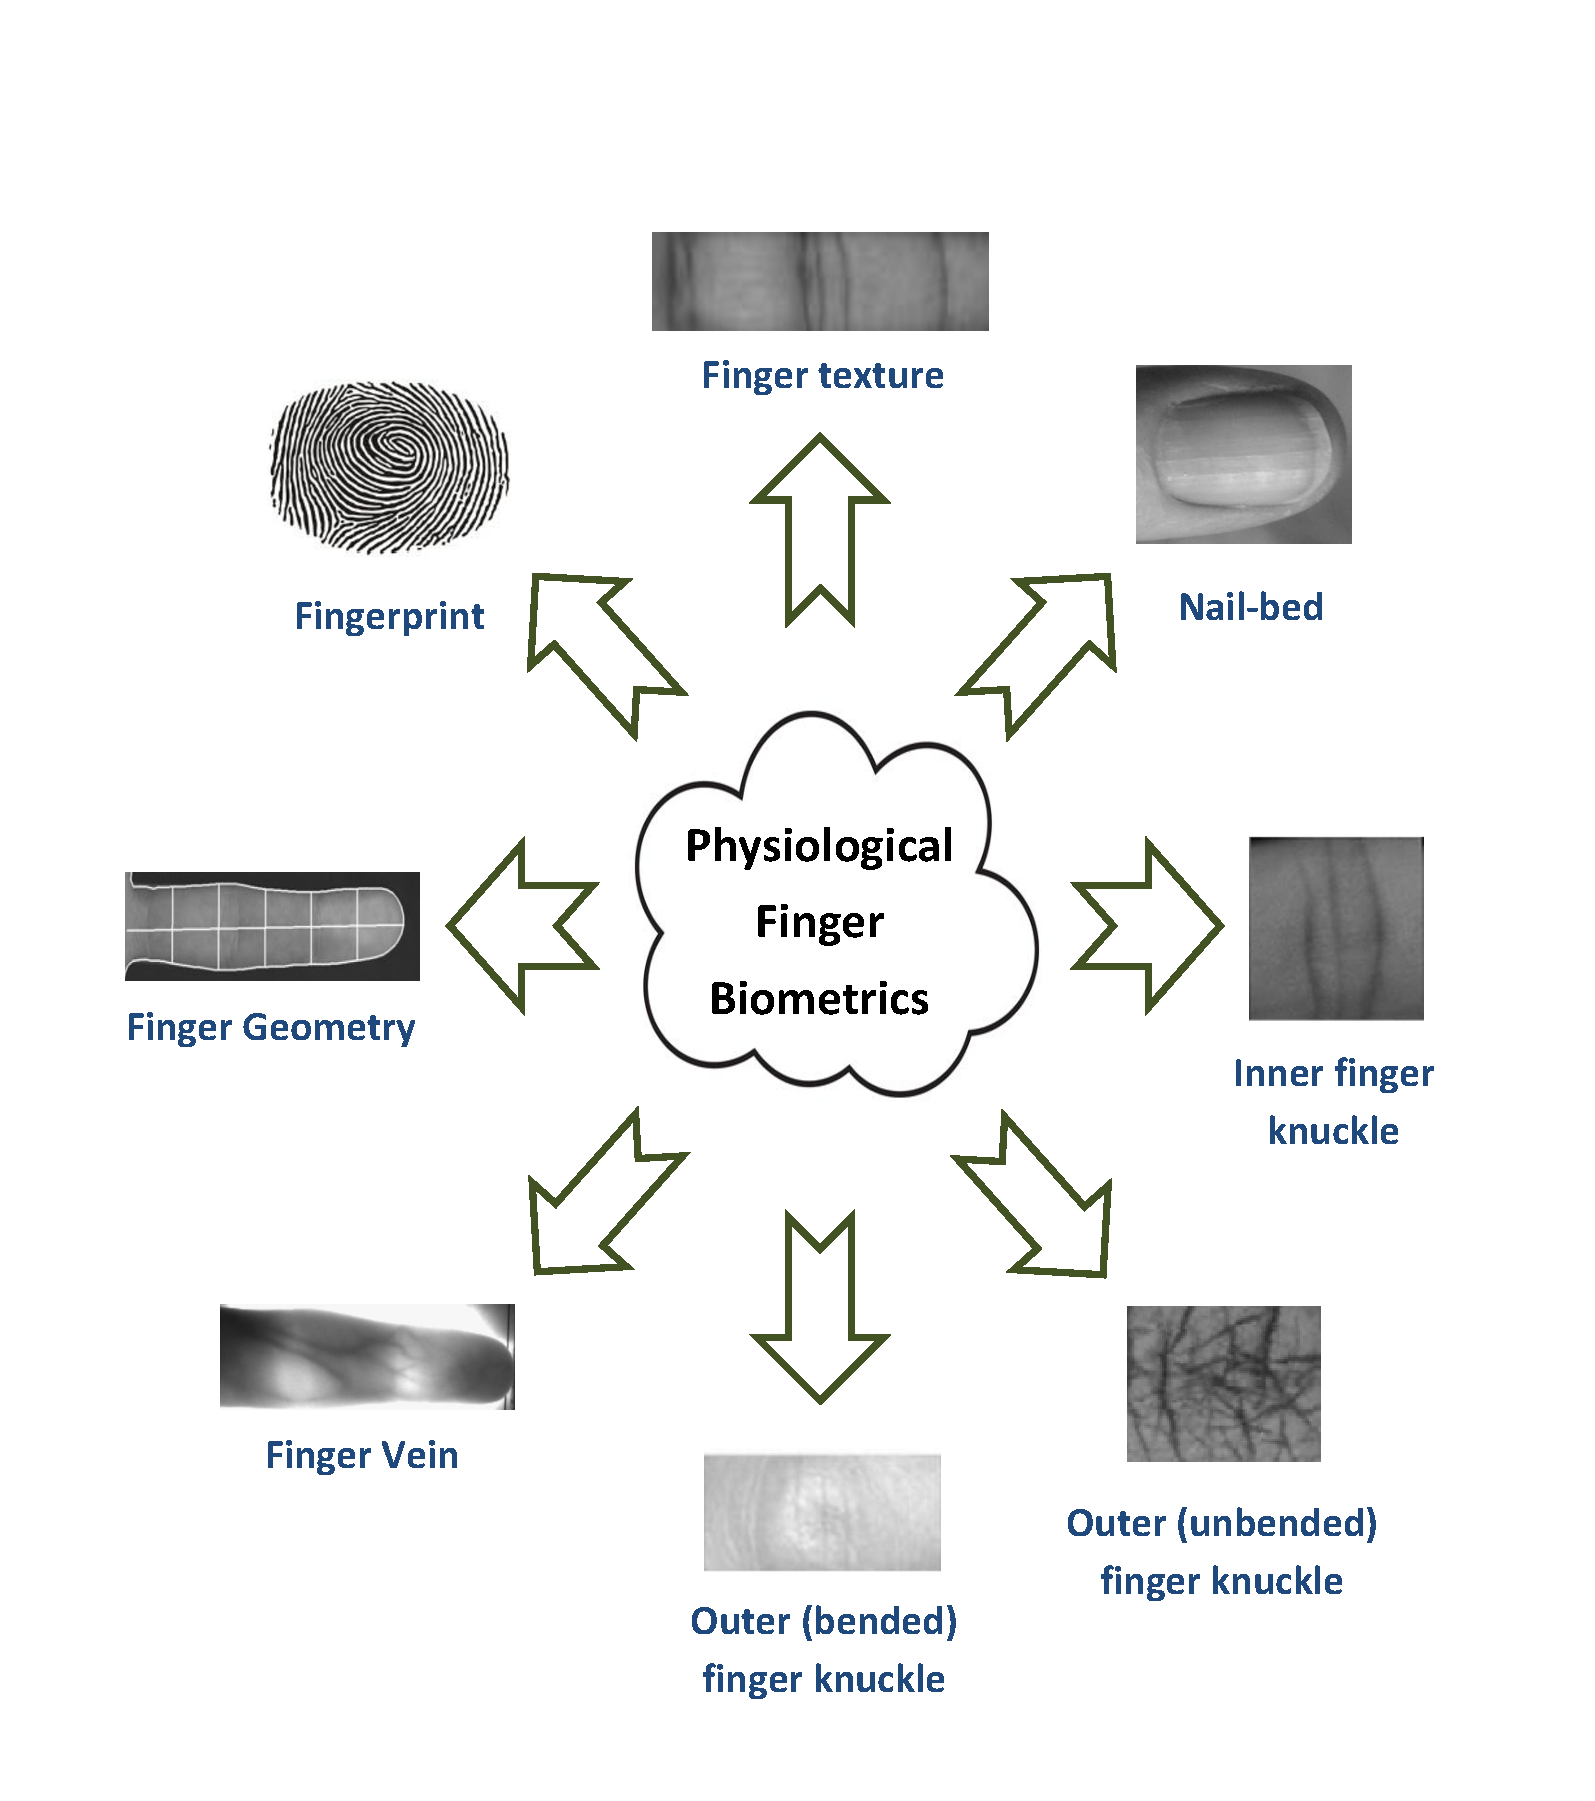
\includegraphics[page=1,scale=.5,trim=2cm 13.5cm 20cm 14cm,clip]{Finger_biometrics.pdf}\end{minipage} & Finger widths and hight \\ \hline
			\textbf{Finger Vein} & \begin{minipage}{0.75\hsize}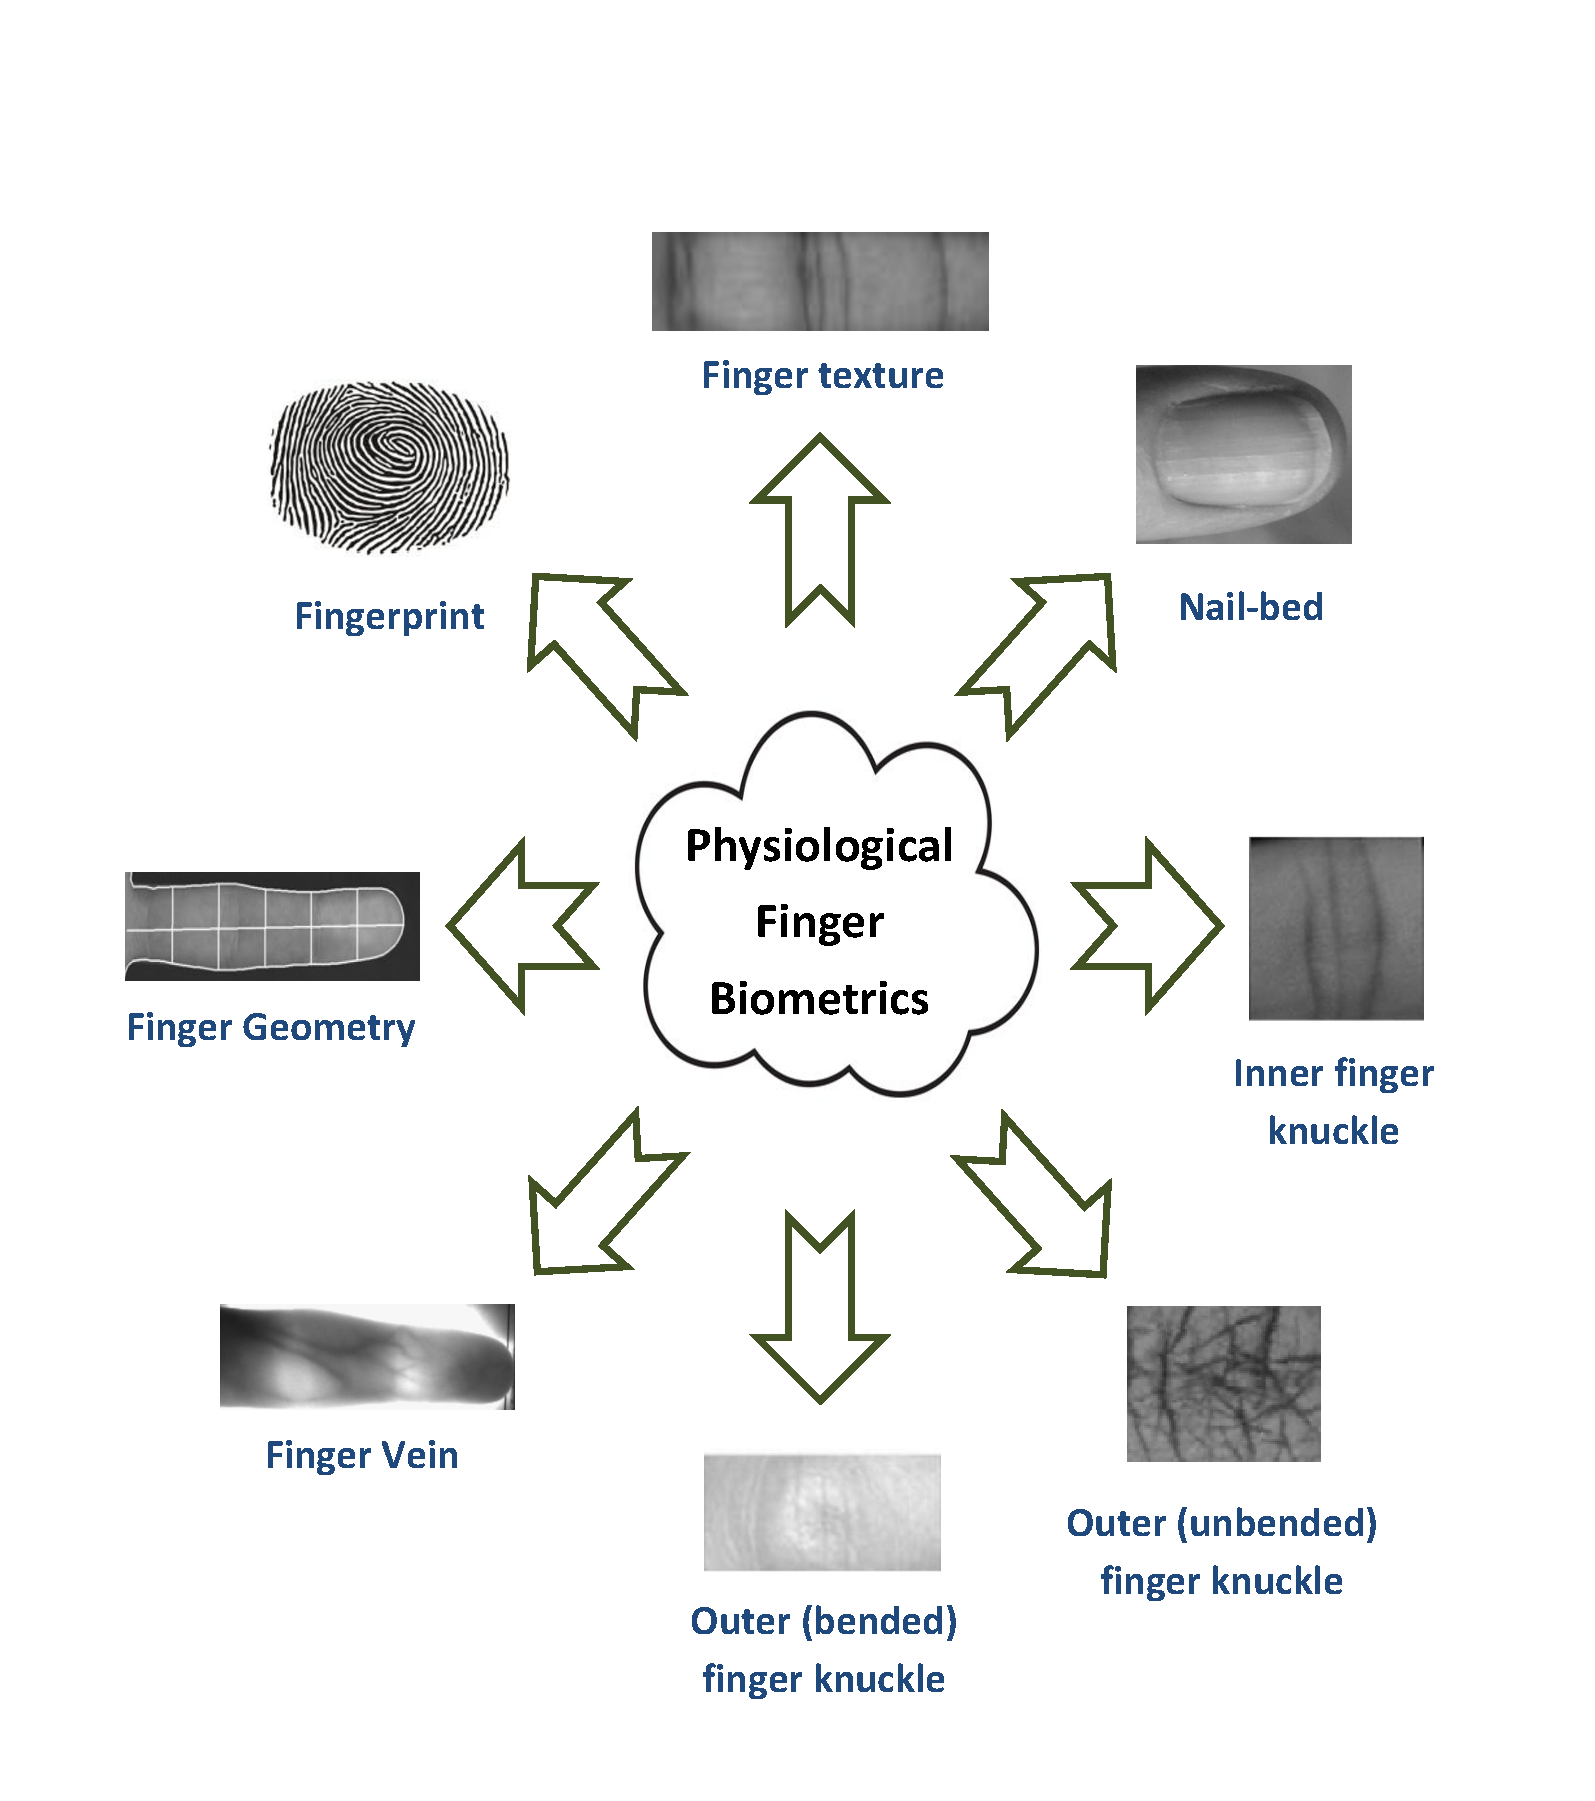
\includegraphics[page=1,scale=.5,trim=3.6cm 6.3cm 18cm 21.5cm,clip]{Finger_biometrics.pdf}\end{minipage} & Veins patterns of finger \\ \hline
		 	\textbf{Outer (bended) finger knuckle}& \begin{minipage}{0.75\hsize}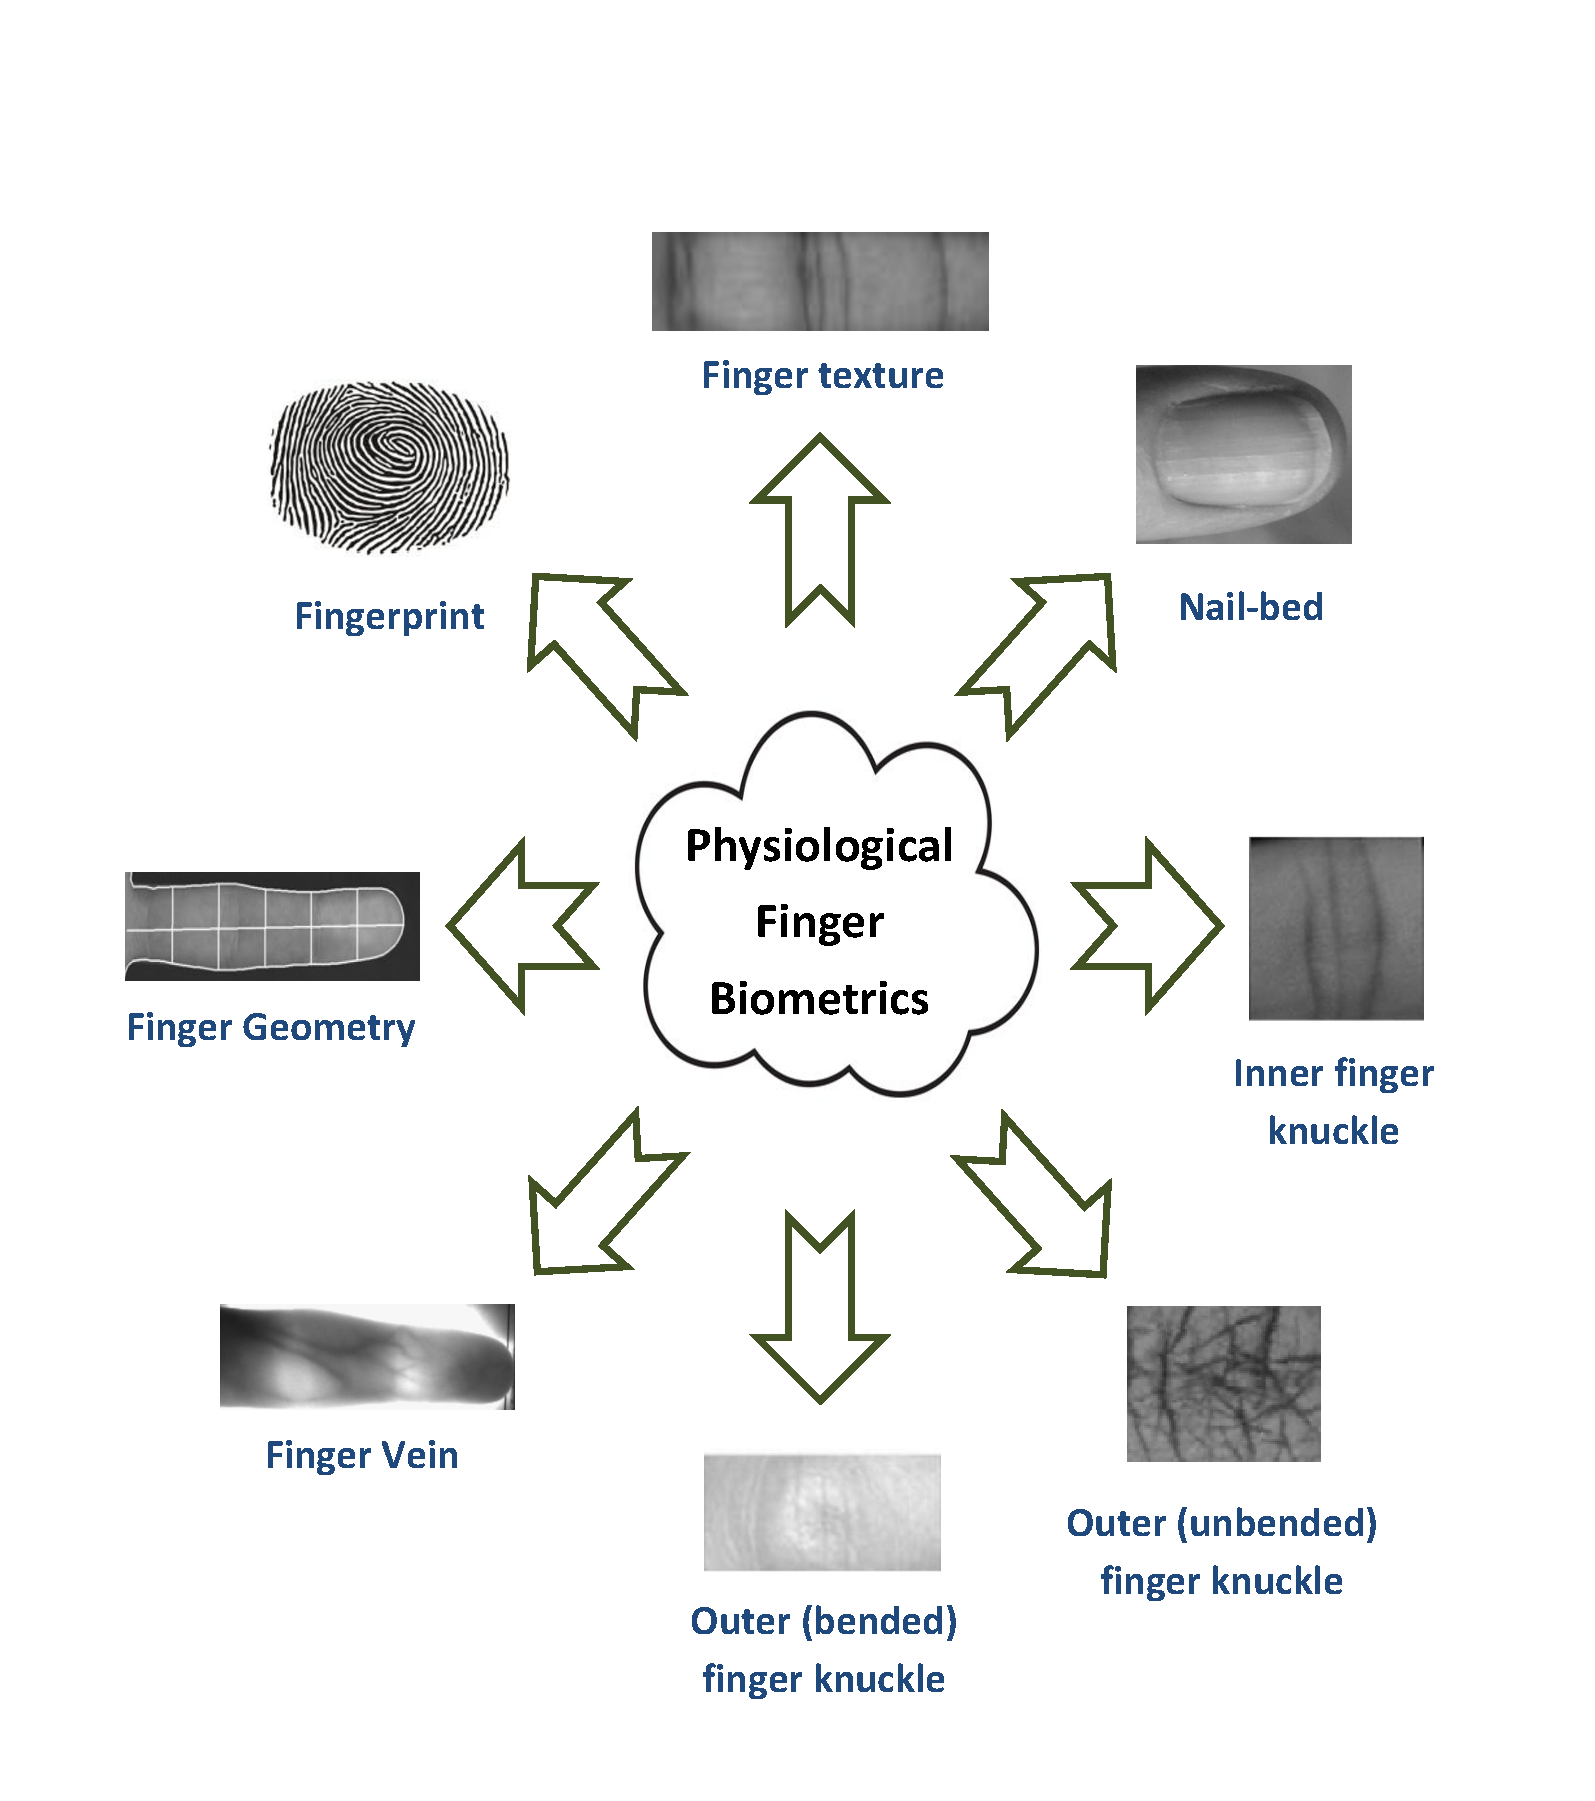
\includegraphics[page=1,scale=.5,trim=11.5cm 3.4cm 10.5cm 24cm,clip]{Finger_biometrics.pdf}\end{minipage} & Major outer surface finger knuckle (bended finger) \\ \hline
			\textbf{Outer (unbended) finger knuckle}& \begin{minipage}{.75\hsize}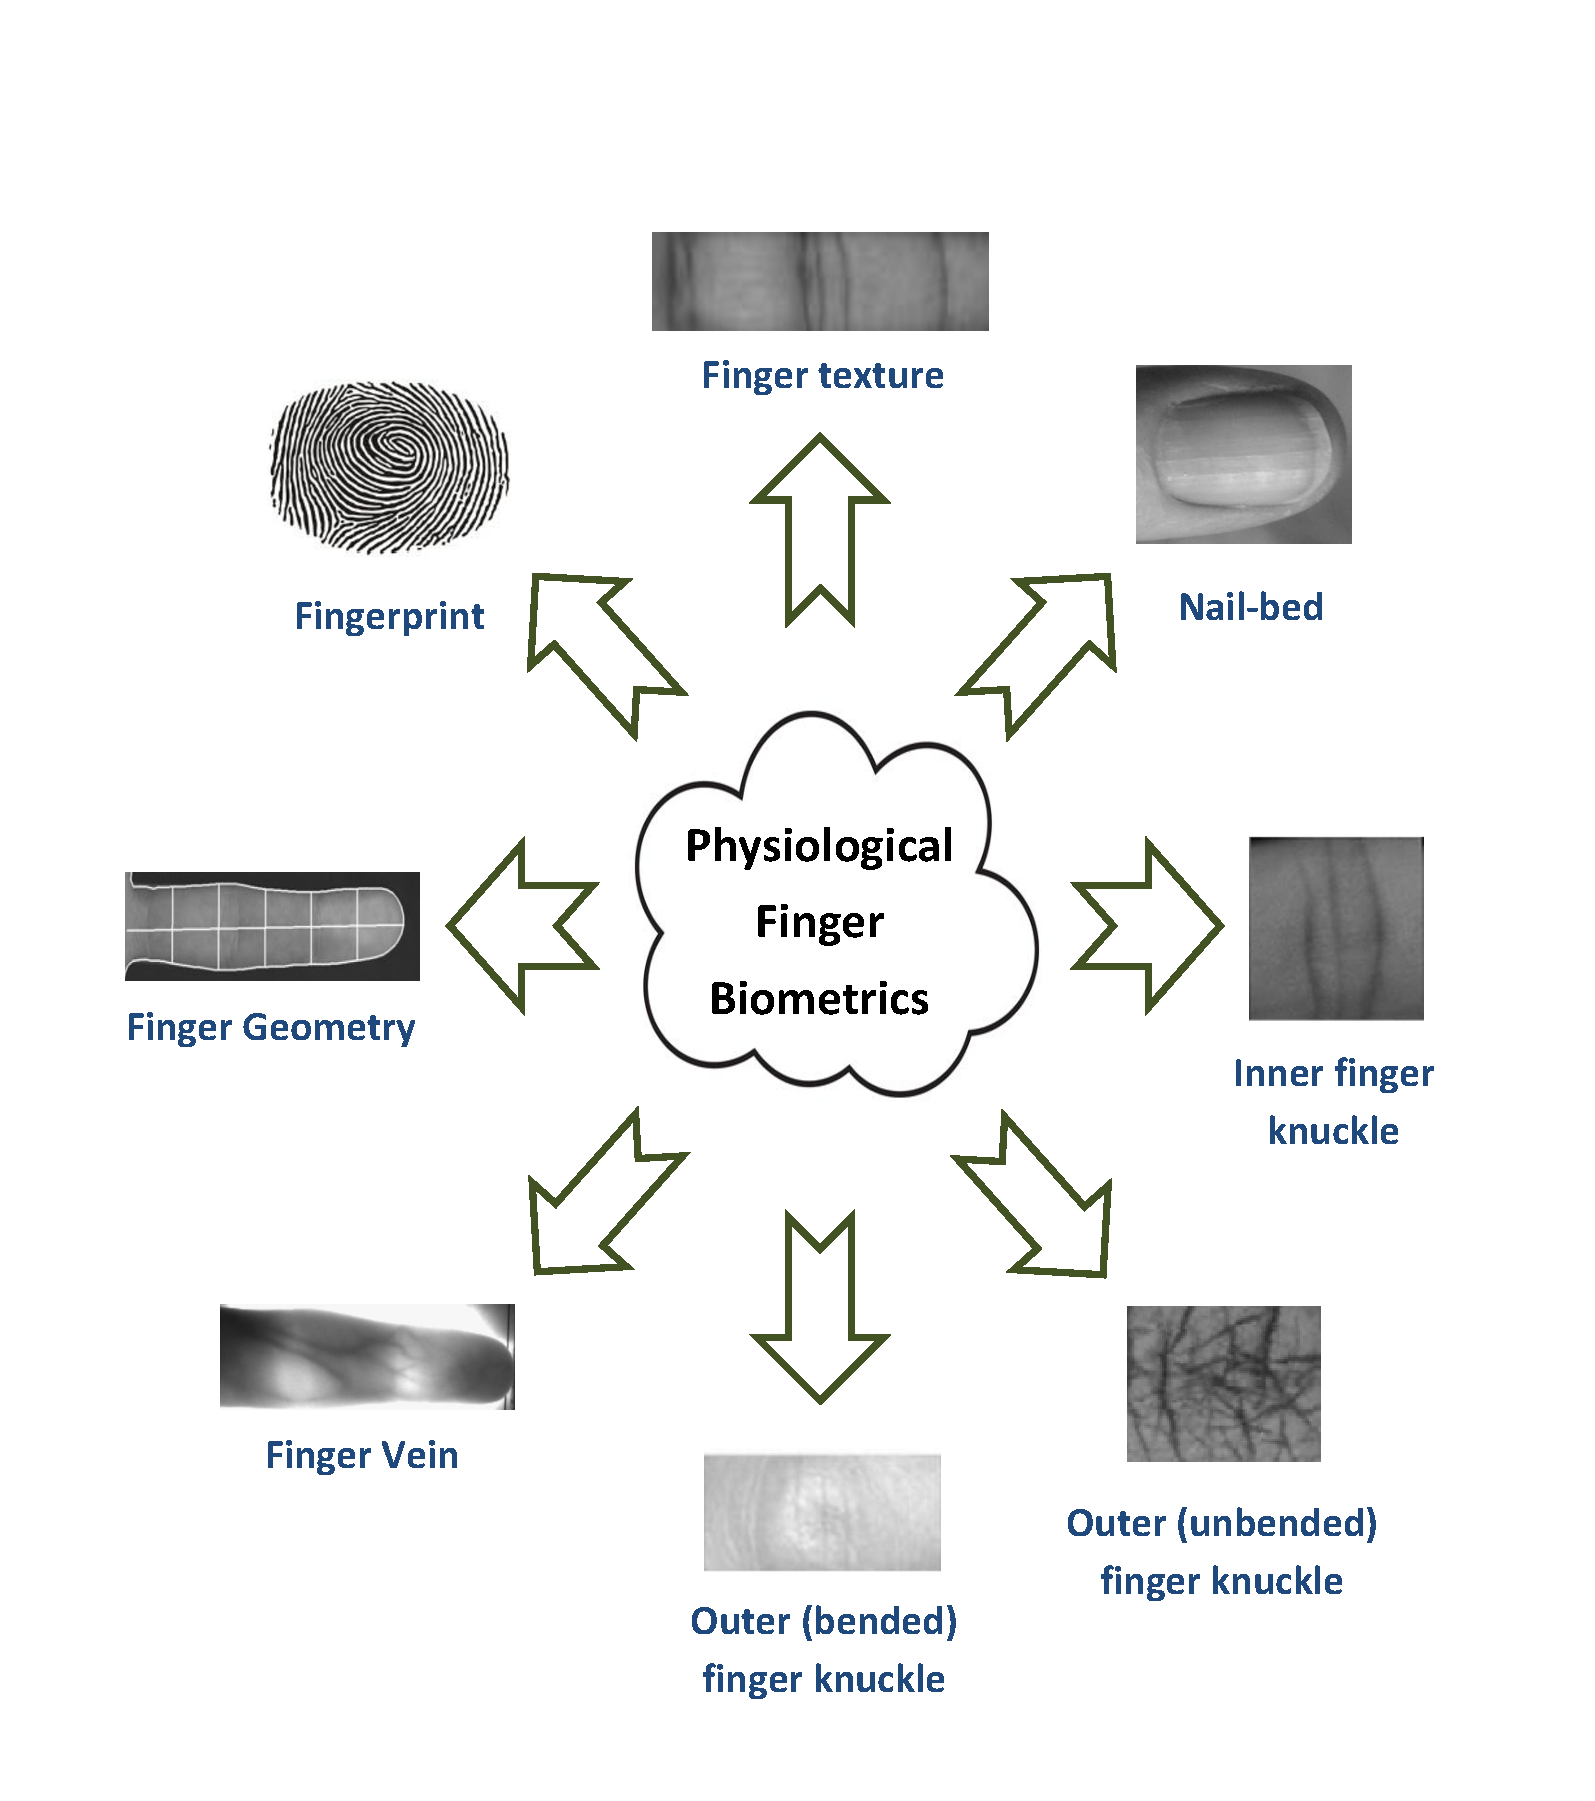
\includegraphics[page=1,scale=.5,trim=18.4cm 5.4cm 2cm 21.6cm,clip]{Finger_biometrics.pdf}\end{minipage} & Major outer surface finger knuckle (unbended finger)\\ \hline
			\textbf{Inner finger knuckle}&~~ \begin{minipage}{0.75\hsize}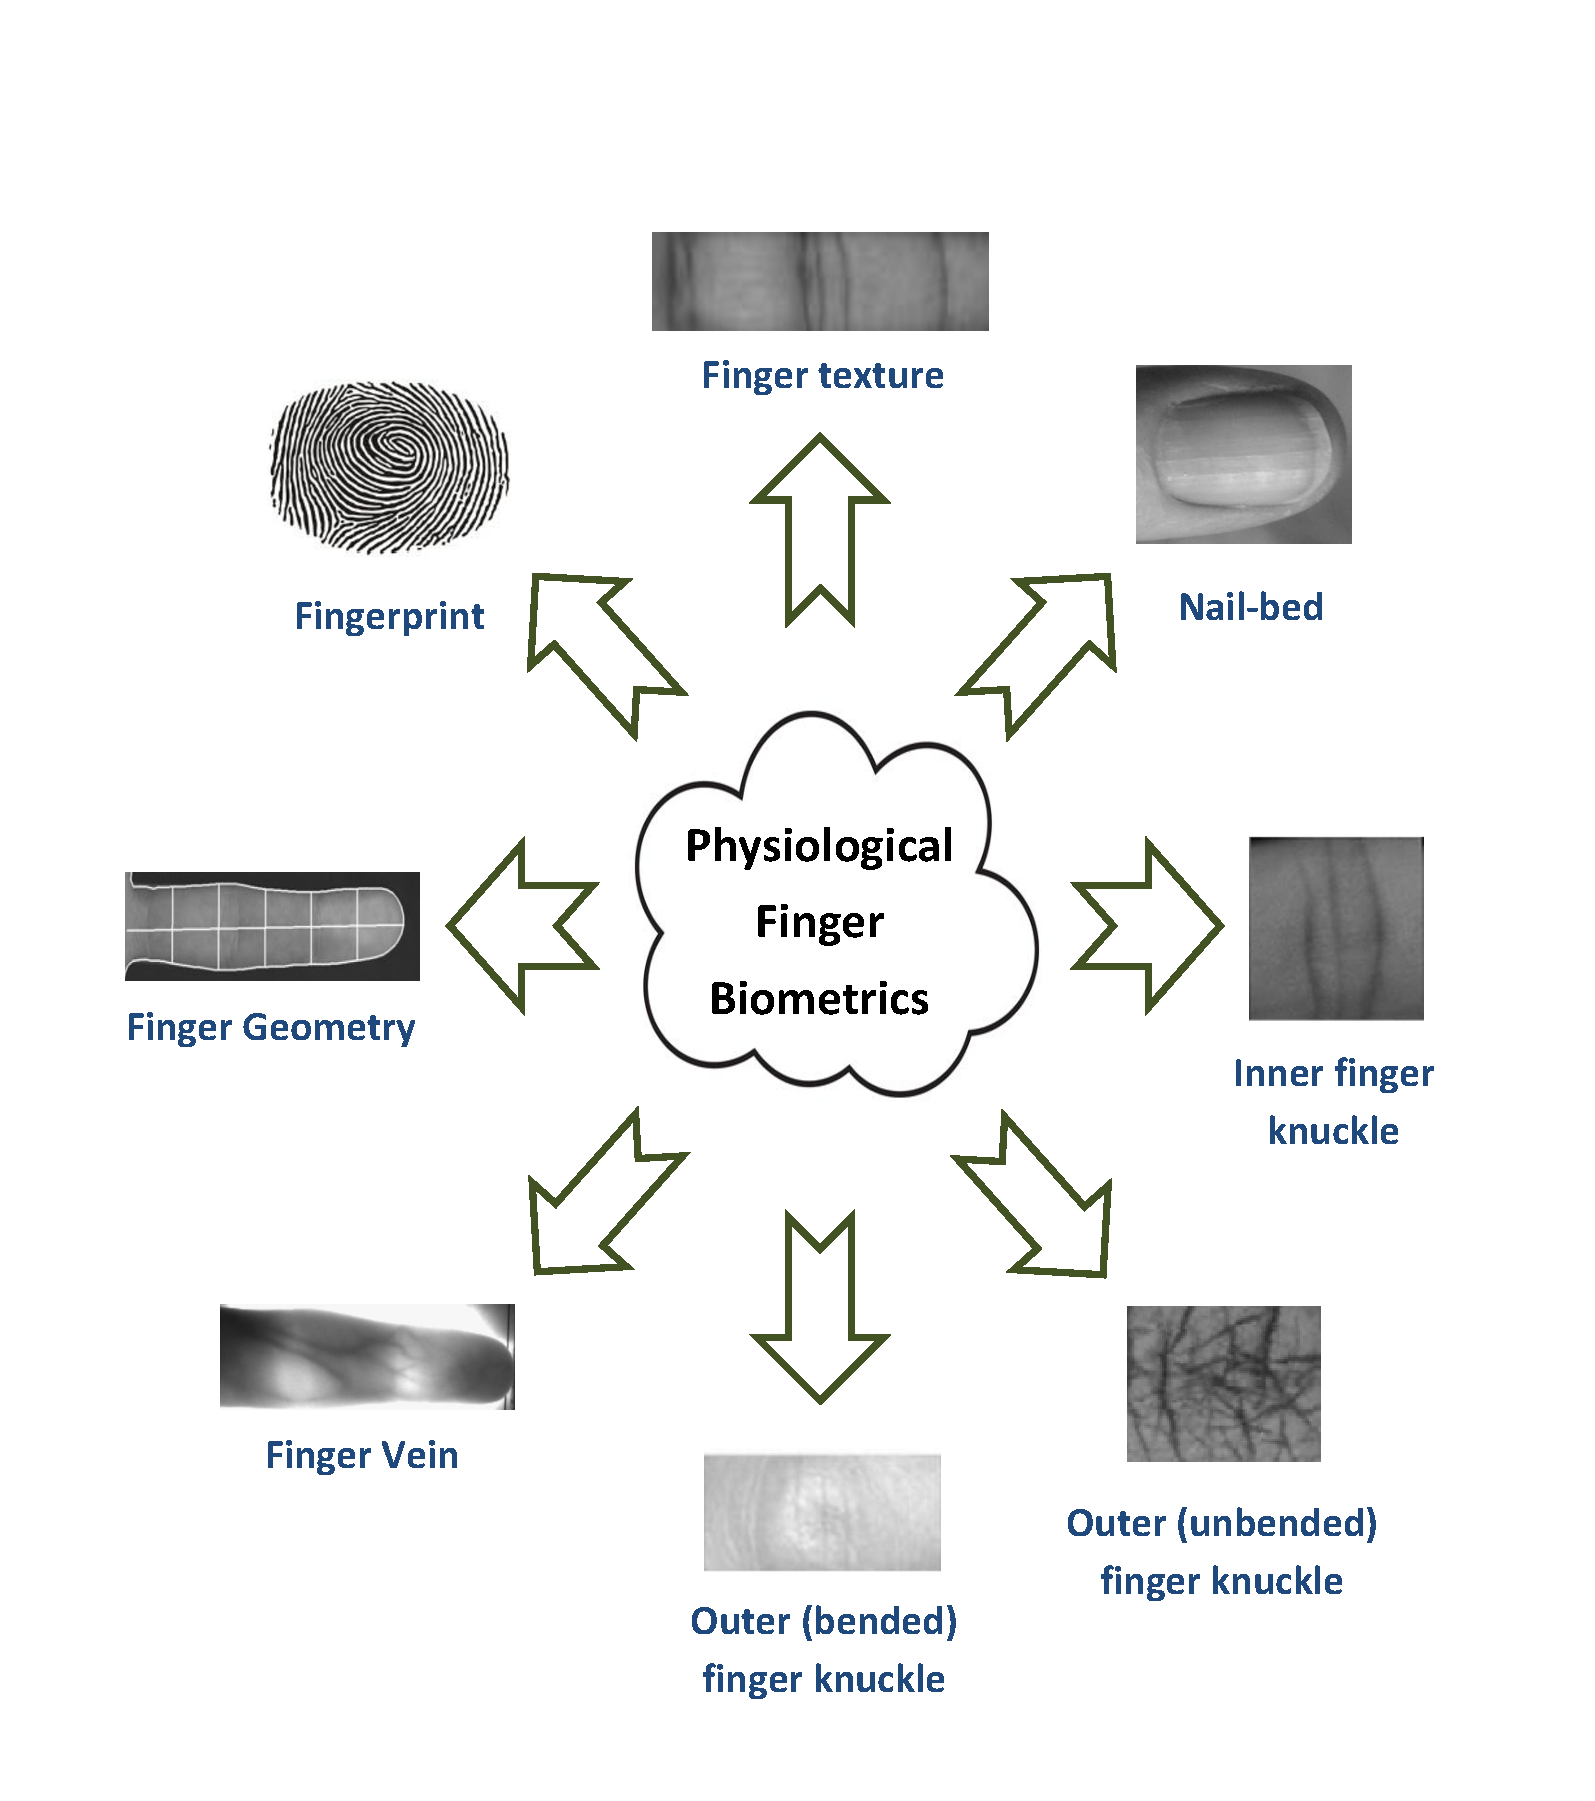
\includegraphics[page=1,scale=.5,trim=20.7cm 12.8cm 1.5cm 13.6cm,clip]{Finger_biometrics.pdf}\end{minipage} & Middle inner surface finger knuckle \\ \hline
			\textbf{Nail-bed}&~ \begin{minipage}{0.75\hsize}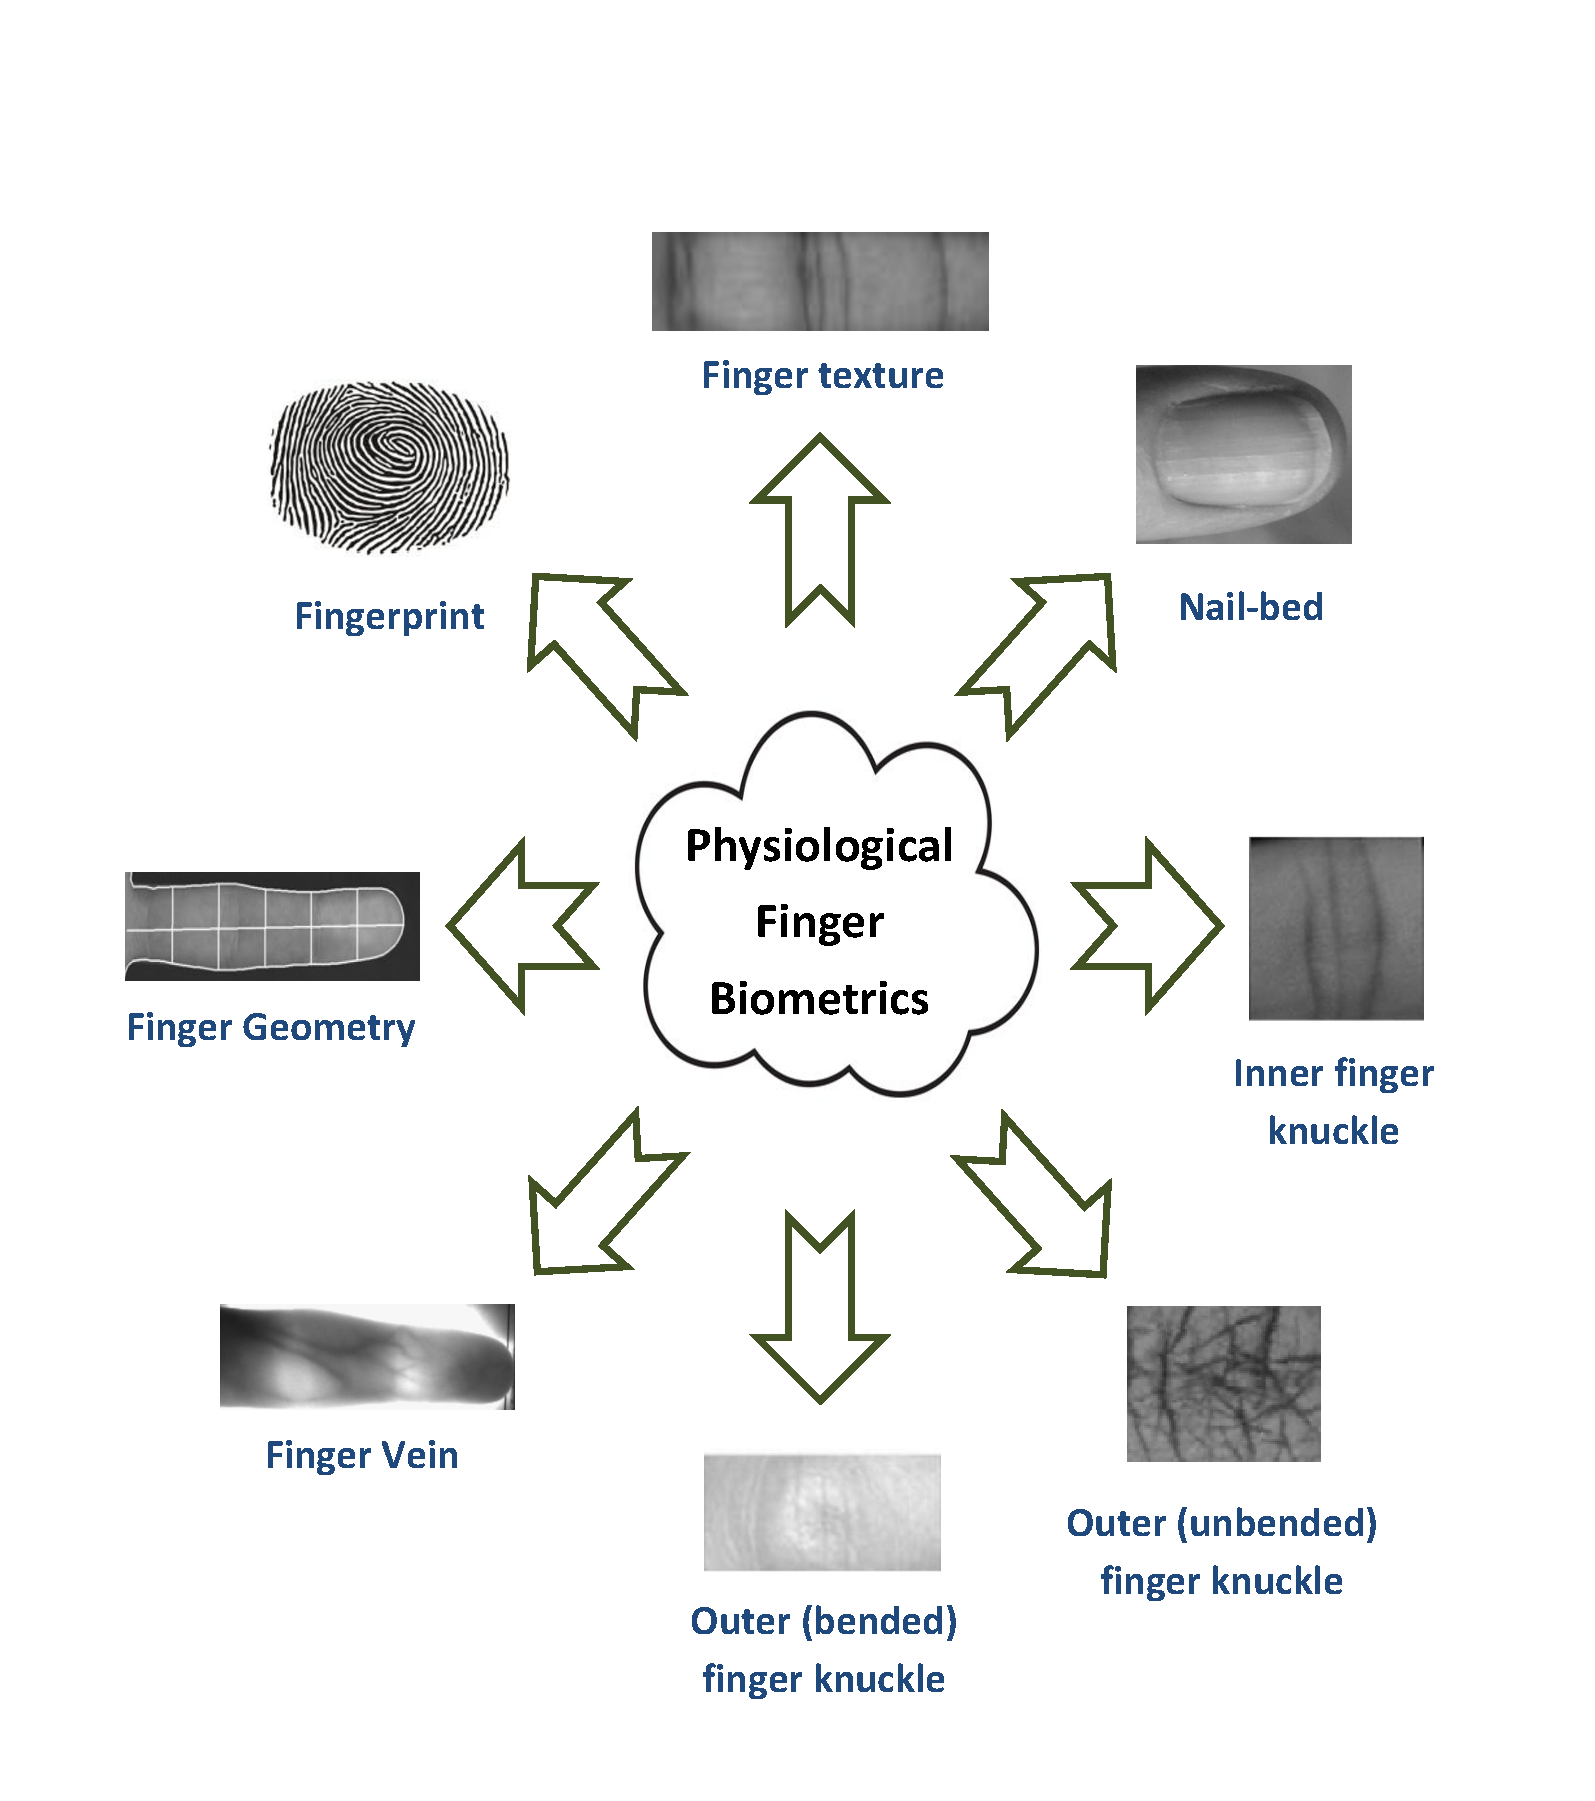
\includegraphics[page=1,scale=.5,trim=19cm 20.8cm 3cm 5.5cm,clip]{Finger_biometrics.pdf}\end{minipage} & Visible nail-bed lines \\ \hline
			\textbf{Finger texture}& \begin{minipage}{0.75\hsize}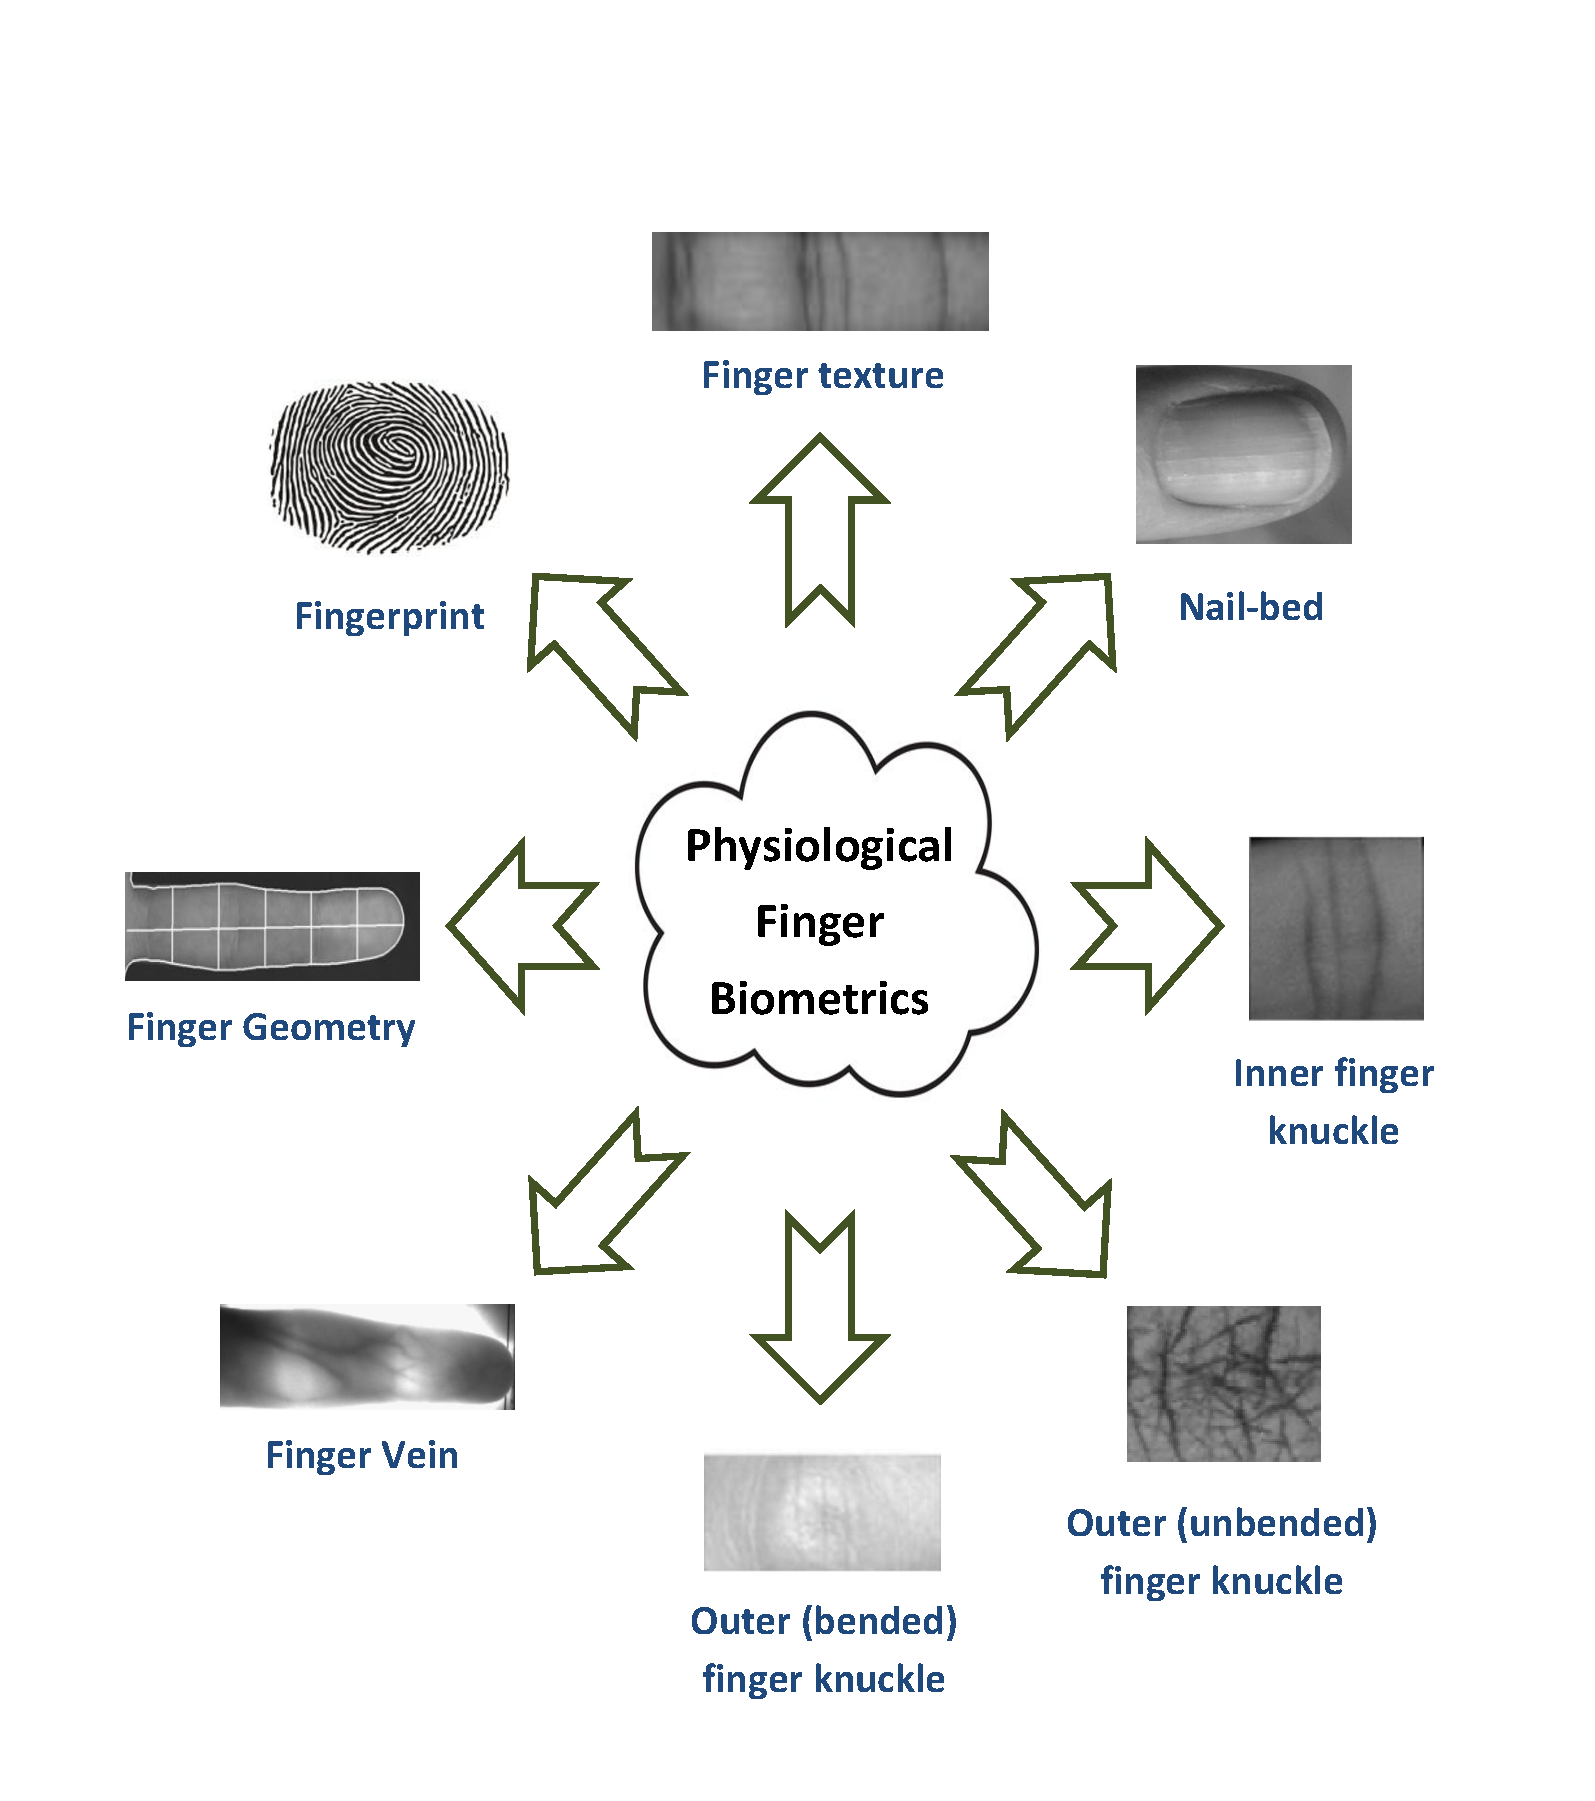
\includegraphics[page=1,scale=.5,trim=11cm 24.4cm 4cm 3.4cm,clip]{Finger_biometrics.pdf}\end{minipage}~~~~~& Inner finger surface, which includes phalanxes and knuckles \\ \hline
	\end{tabular}}
\end{table}


%	\begin{figure}[!b]
%		\centering
%		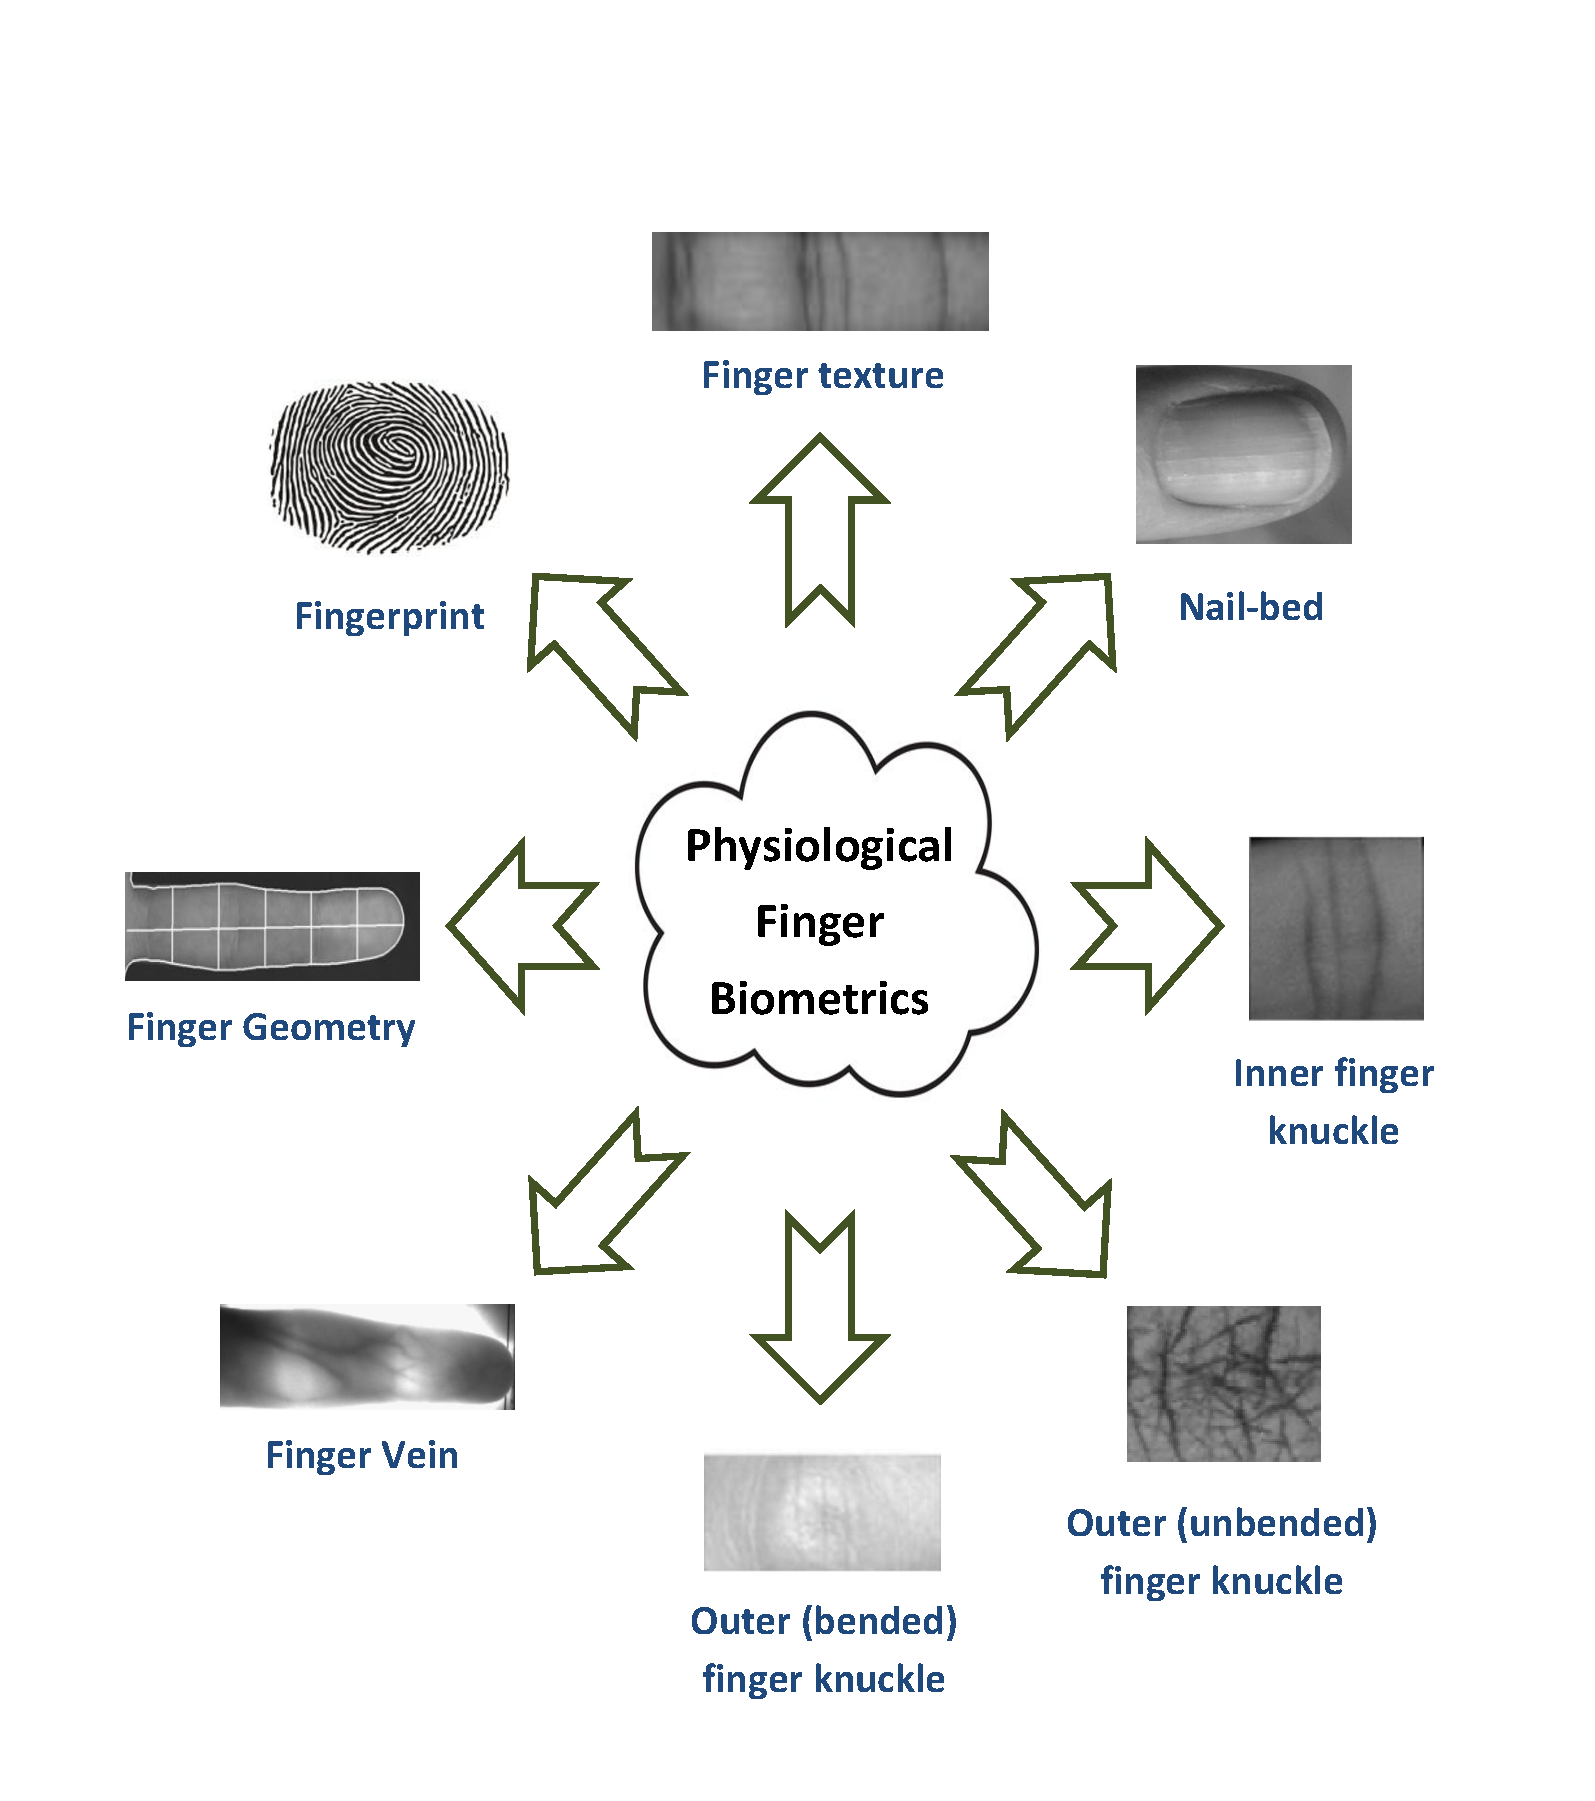
\includegraphics[page=1,scale=.51,trim=0cm 0cm .6cm 3cm,clip]{Finger_biometrics.pdf}
%		\caption{Different physiological characteristics that can be found in each single finger}
%		\label{fig:Physiological_biometrics}
%	\end{figure}
	\begin{figure}[!h]
		\centering
		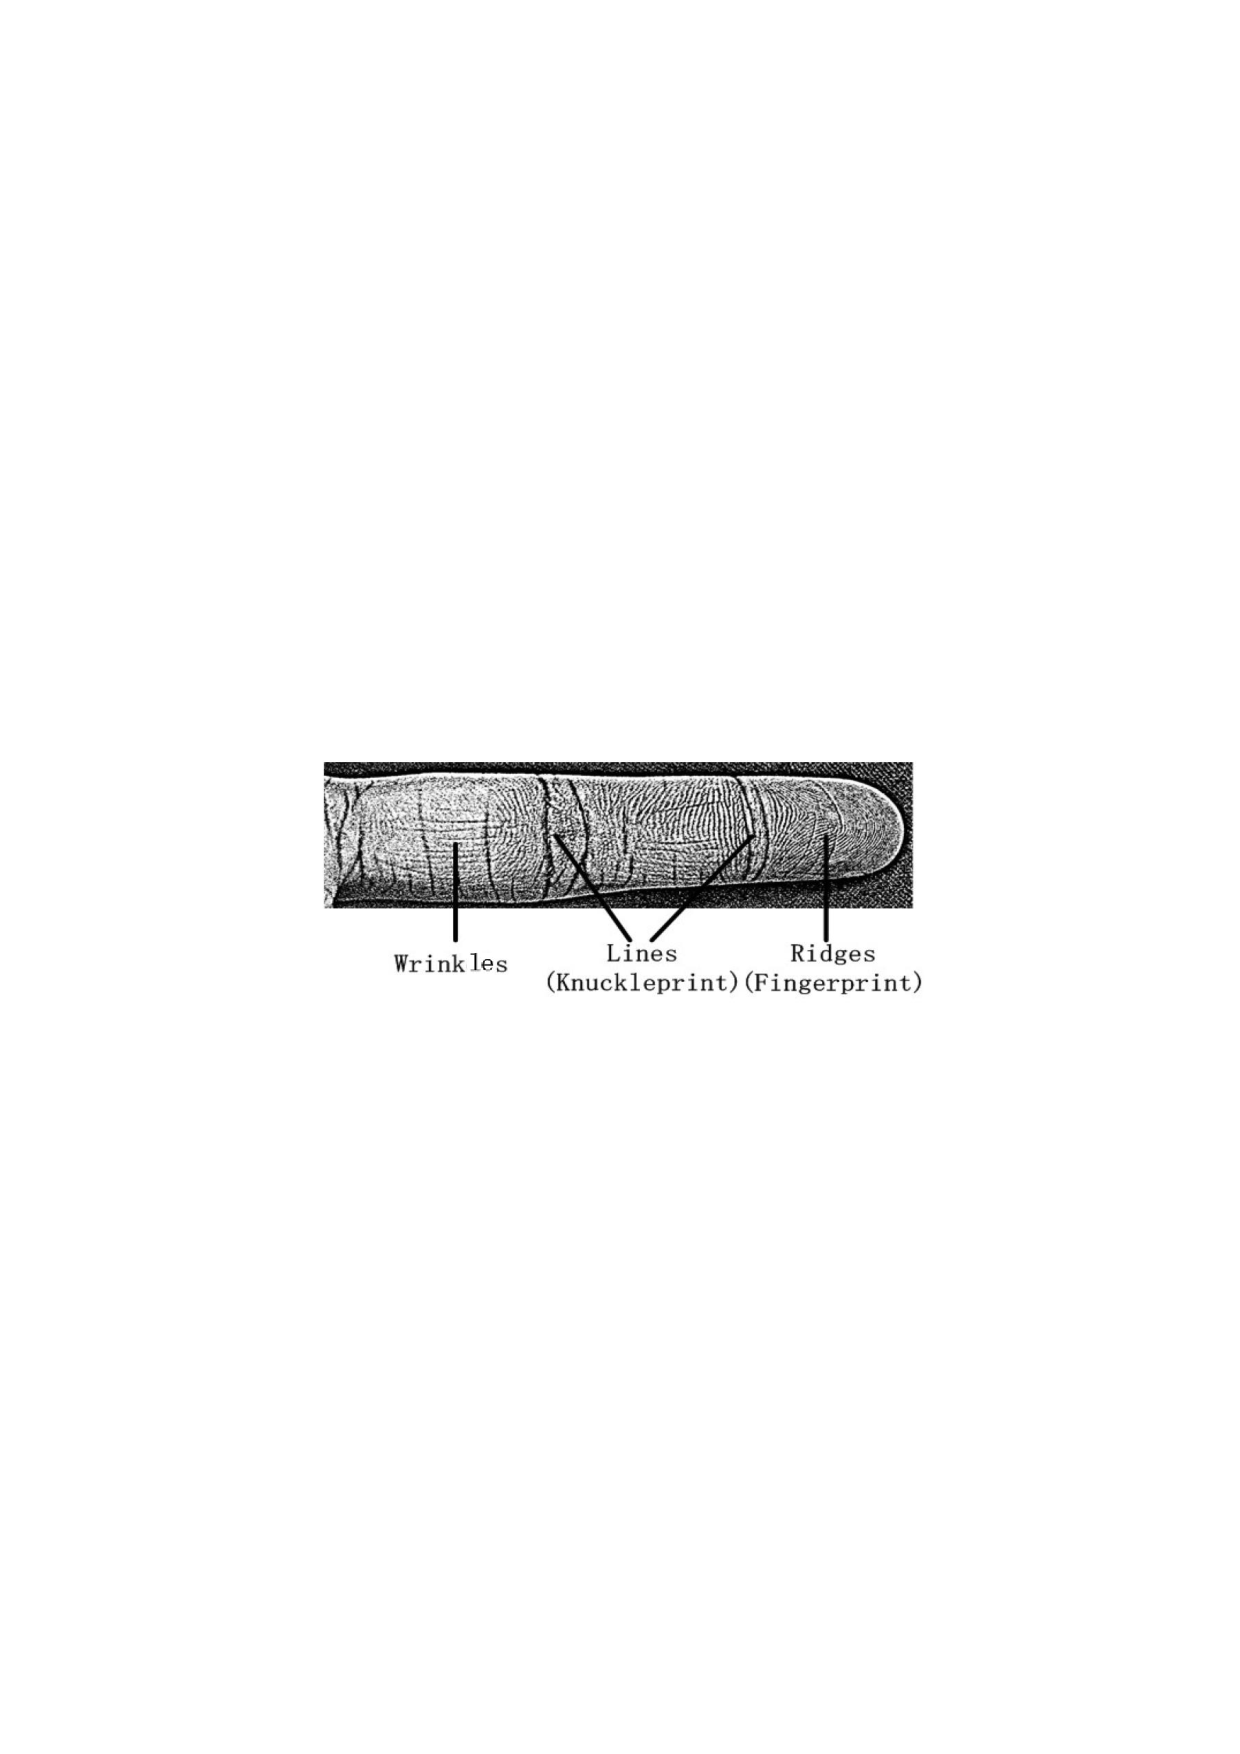
\includegraphics[scale=.7,trim=4cm 12.5cm 4cm 12cm,clip]{FT2.pdf}
		\caption{Various patterns that formed the inner surface of a finger: ridges, visible lines and skin wrinkles as given in \cite{li2004personal}}	\label{fig:FT2}
	\end{figure}
	\begin{figure}[!h]
		\centering
		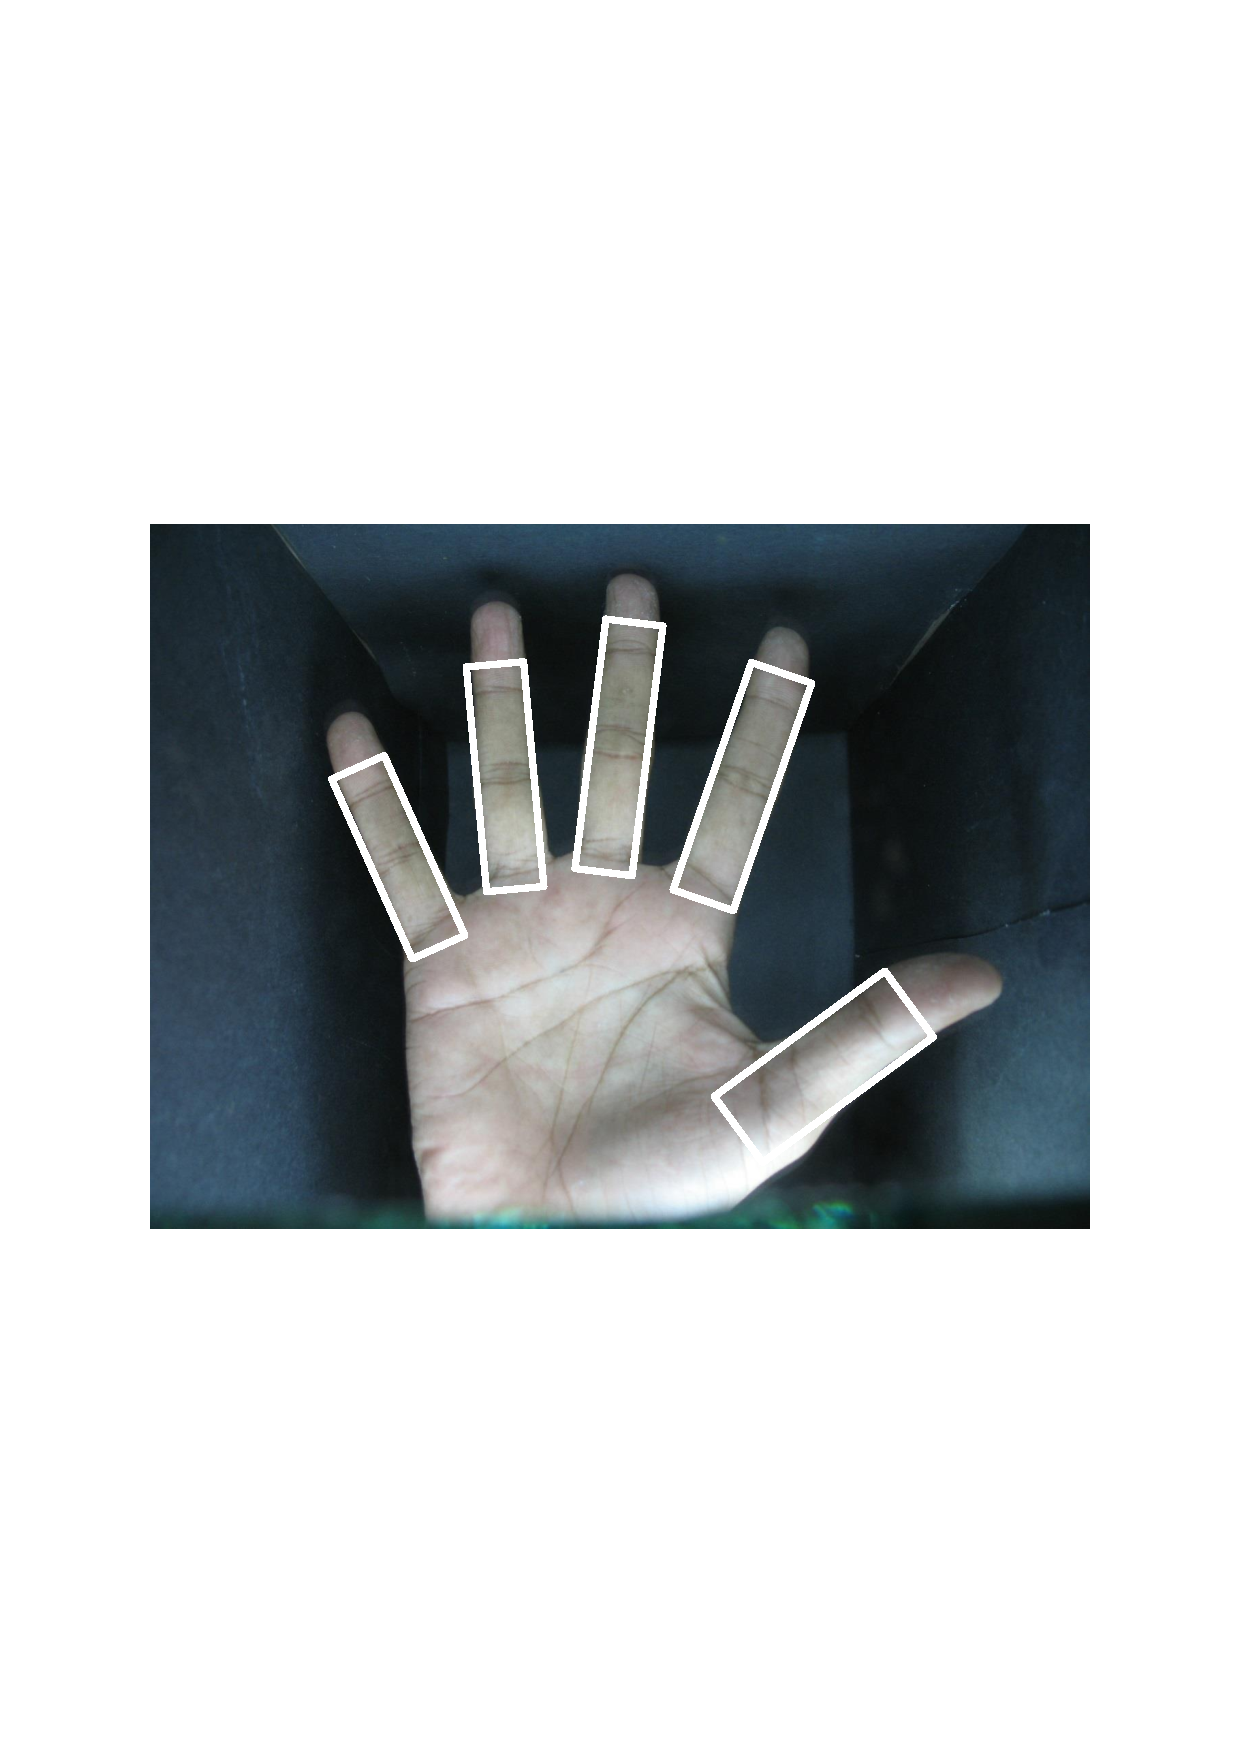
\includegraphics[page=1,scale=.7,trim=3cm 8cm 3cm 8cm,clip]{FTs_locations.pdf}
		\caption{The main positions of the FTs \hl{(assigned by the white rectangles). Essentially, as explained in} \cite{Al-Nima2017Signal} they can be found in the inner hand surface of the five fingers and they are located between the upper phalanx (below the fingerprint) and the lower knuckle (the base of the finger)}
		\label{fig:FTs_locations}
	\end{figure}
	%In the case of the FT literature review, few works have utilized the FT as a biometric type. The idea of using this important biometric only appeared approximately one decade ago. Because an FT recognition system is generally compromised within the following steps: finger segmentation and FT collection; feature extraction; matching classifier (multi-object fusion could be used in this stage) and recognition performance, related work will be reviewed for each step. \\

	FT area involves phalanx and knuckle patterns. For a full FT region, three phalanxes and three knuckles can be recognised on the inner surface of a little; ring; middle or index finger, and two phalanxes and two knuckles on the inner surface of a thumb. 
	
	\hl{The three types of phalanxes for the four fingers are: (1) upper phalanx (below the fingerprint) called distal; (2) middle phalanx named intermediate and (3) lower phalanx termed proximal.} 
	
	\hl{The three types of knuckles for the four fingers are: (1) upper knuckle between the distal and intermediate phalanxes; (2) middle knuckle between the intermediate and proximal phalanxes and (3) lower knuckle near the palm.} 
	
	\hl{The two types of phalanxes for the thumb are: (1) upper phalanx (below the fingerprint) called distal and (2) lower phalanx termed proximal.} 
	
	\hl{The two types of knuckles for the thumb are: (1) upper knuckle between the distal and (2) intermediate phalanxes and lower knuckle near the palm.} 
	
	FT patterns are structured before the birth. The FTs can provide high recognition performance due to their different patterns in their different parts. The principal parts of the FT for a single finger are demonstrated in Fig. \ref{fig:FT_midd_thumb}.
	\begin{figure}[!h]
		\centering
		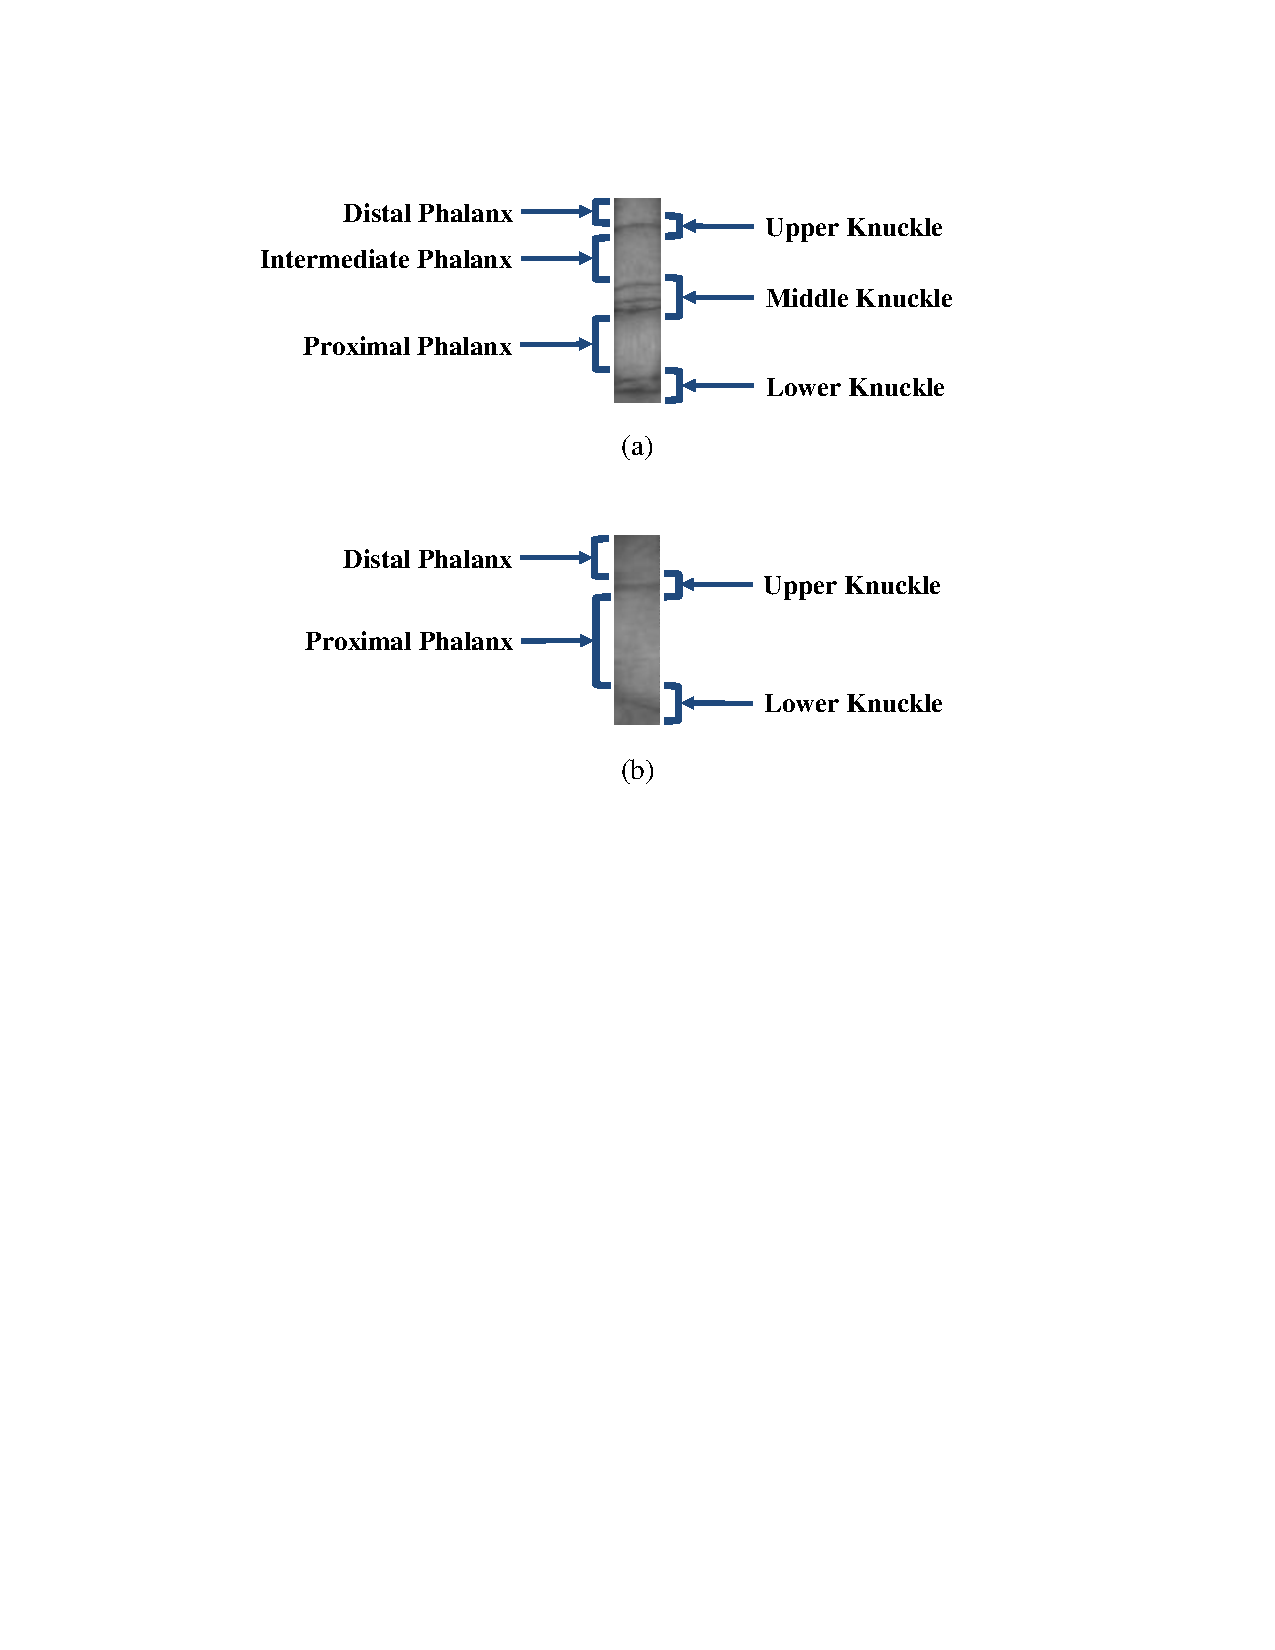
\includegraphics[page=1,scale=1.1,trim=4cm 14cm 4cm 3cm,clip]{FT0.pdf}
		\caption{\hl{Example of the full FT parts in:
		(a) a middle finger (three phalanxes and three knuckles)
		(b) a thumb (two phalanxes and two knuckles)}}	\label{fig:FT_midd_thumb}
	\end{figure}
	%All the FT patterns (excluding the ridges) can be obtained from low cost devices and contactless hands. \\

	The aim of this paper is (1) to provide comprehensive survey for the FT phenomenon in the case of biometric recognitions; (2) to determine the main advantages and drawbacks of prior FT studies and the available FT databases; (3) to suggest insightful future directions to further improve the FT work.  

	The rest of this paper is organized as follows: Section 2 describes the specifications of the finger characteristics and provide their comparisons with the FT; Section 3 highlights the main recognition system stages that were considered in the FT studies; Section 4 illustrates the finger segmentation and FT collection studies; Section 5 states the employed FT feature extraction techniques; Section 6 reviews the multi-object fusion of FT work; Section 7 explains the utilized and available FT databases; Section 8 surveys FT recognition performances and Section 9 concludes the paper with presenting suggestions for future studies.

\section{FT Anatomy and Comparison with Other Physiological Finger Characteristics}
	To present comprehensive study and show the effectiveness of the FTs, \hl{general overview for different physiological finger characteristics will be provided;} their benefits and drawbacks will be illustrated; and comparisons with the FTs will be highlighted.
	\paragraph{\textbf{Fingerprint:}} Fingerprints have been studied for many years and can be considered as the first effective physiological biometric. They have been employed in many biometric fields such as classification \cite{Halici1996Fingerprint}, verification \cite{Gil2013Fingerprint}, identification \cite{Bifari2014Automated} and multi-modal recognition \cite{Conti2010AFrequency}. Fingerprints are constructed from different pattern forms. 
	These patterns consist of \hl{constructive} features such as valleys/ridges, core-points and minutiae \cite{mukhaiyar2015cancellable}. The most important advantage of this biometric compared with other finger patterns is that \hl{a fingerprint can be collected from its trace (fingermark)}. This facilitates the forensic investigations of crimes \cite{Makrushin2015Forensic,Kotzerke2015Discriminating,Merkel2014Latent,Ezeobiejesi2016Latent,Zhang2014Adaptive,Paulino2013Latent}. However, biometric systems based upon fingerprints have obstacles. For example, it has been reported that recognition rates of fingerprints are generally reduced when the individual becomes older \cite{Modi2007Impact}. Furthermore, it has been noticed that fingerprint patterns may vanish for elderly people especially those suffering from diabetes \cite{kabadi1991classification}. Therefore, this will cause erroneous results in biometric systems. 
	
	In contrast to the FT, the visible lines and skin wrinkles of the FT are more reliable and permanent \cite{Al-Nima2017Signal}. The FT horizontal and vertical patterns can be acquired by using low resolution acquisition devices. In addition, the FT region is bigger than the fingerprint region, therefore, it provides more features that are useful for personal recognitions. 
	\paragraph{\textbf{Finger Geometry (FG):}} The geometry of fingers is an important part of hand geometry as described in \cite{Sanchez-Reillo2000Biometric,Ayurzana2013Astudy,Svoboda2015Contactless}. Several recent studies considered FG alone as a type of biometric characteristic such as in \cite{Malassiotis2006Personal,Aghili2010Personal,Liu2015Hand}. Generally, to extract the geometry features of a single finger, multiple widths to determine locations along with the finger length are utilized in verification/identification systems. 
	%	\begin{figure}[!h]
	%		\centering
	%		\includegraphics[page=1,scale=.75,trim=2cm 7cm 2cm 7cm,clip]{finger_geometry.pdf}
	%		\caption{Common finger geometry features of the four fingers, where these are for each single finger: multiple finger widths in assigned locations and finger length \cite{Ribaric2005Anonline}}
	%		\label{fig:finger_geometry}
	%	\end{figure}
	The following issues need to be considered with the FG characteristic: an appropriate binarization threshold for a hand image is required \cite{Kang2014Pose}, pegs or restrictions in the acquisition device can influence the measured shape of any finger(s) and the security level of FG systems may not be high \cite{Aghili2010Personal}. To increase the performance of the FG, additional biometrics are generally employed in the proposed recognition schemes. For instance, single finger patterns of FV and FG were fused together in \cite{Kang2010Multimodal}. Another example, the palmprint was combined with the FG in \cite{Yu2010Feature,Joshi2014Enhancing,Anitha2014Anovel}. 
	
	In contrary to the FT, the security level that provided by the FT is very high \cite{Ribaric2005ABiometric,Al-Nima2017Robust,Al-Nima2017Signal}. Pegs or restrictions in the acquisition device can be used and they are not required at the same time. This is because that the boundary of a finger does not significantly affect the features or the \hl{Region Of Interest (ROI)} of the FT. \hl{Moreover, the FTs of different fingers can be exploited together to produce a high recognition biometric system} \cite{Al-Nima2017Robust,Al-Nima2017finger, Al-Nima2017Signal}\hl{, therefore, fusions or combinations with other biometric characteristics are not important to be considered.} 
	\paragraph{\textbf{Finger Vein (FV):}} \hl{FV is a biometric pattern that commonly positioned close to the proximity of the skin of a hand} \cite{hartung2012vascular}. It provides a high degree of confidentiality as it is so difficult to steal or use without a human's awareness. Furthermore, it can be only acquired when the individual is alive and this increases the spoofing difficulties of this biometric type \cite{Kumar2012Human}. \hl{Such a biometric requires a specific Near-InfraRed (NIR) environment in the acquisition system}. Moreover, it has been cited that changing the position of the camera around a finger offers different views of veins and this can be beneficial to capture various FV patterns \cite{Lu2014Finger}. \hl{Different finger bending degrees afford various FV features too.}
	%	\begin{figure}[!h]
	%		\centering
	%		\includegraphics[page=1,scale=.6,trim=2cm 7.5cm 2cm 7cm,clip]{acquisition_finger_vein.pdf}
	%		\caption{Example of an acquired FV environment \cite{Liu2012AnEmbedded}}
	%		\label{fig:acquisition_finger_vein}
	%	\end{figure}
	One of the main FV biometric problems is the difficulty of capturing distinct vein features. Therefore, \hl{unclear patterns (because of undistributed illumination)} or wrongly located fingers can increase the false recognition performance \cite{Lee2009Restoration}. 
	%	\begin{figure}[!b]
	%		\centering
	%		\includegraphics[page=2,scale=.6,trim=3cm 20cm 3cm 2cm,clip]{finger_veins.pdf}
	%		\caption{FV image of an index finger}
	%		\label{fig:finger_veins1}
	%	\end{figure}
	%	\begin{figure}[!t]
	%		\centering
	%		\includegraphics[page=1,scale=.6,trim=3cm 20cm 3cm 2cm,clip]{finger_veins.pdf}
	%		\caption{FV image of an index finger shows parts of veins disappeared because of over illumination}
	%		\label{fig:finger_veins2}
	%	\end{figure}
	%	\begin{figure}[!t]
	%		\centering
	%		\includegraphics[page=4,scale=.6,trim=3cm 20cm 3cm 2cm,clip]{finger_veins.pdf}
	%		\caption{FV image of a middle finger}
	%		\label{fig:finger_veins3}
	%	\end{figure}
	%	\begin{figure}[!t]
	%		\centering
	%		\includegraphics[page=3,scale=.6,trim=3cm 20cm 3cm 2cm,clip]{finger_veins.pdf}
	%		\caption{FV image of a middle finger shows parts of veins disappeared because of over illumination}
	%		\label{fig:finger_veins4}
	%	\end{figure}
	It can be investigated that available FV acquiring devices offer capturing one image for a single finger at a time such as \cite{Zhang2006Multiscale,Wang2010User,Kang2010Multimodal,Kumar2012Human,Liu2012AnEmbedded}, except in \cite{Lu2014Finger} where two camera devices have been used to simultaneously collect two finger images (one from each hand). The index finger, and sometimes the middle finger, is usually used in these devices. Furthermore, some of the captured FV images cannot cover the whole finger as in \cite{Kang2010Multimodal,Wang2010User}. So, not all of the possible FV patterns for all fingers are provided. Therefore, it could be argued that the obtained recognition performance can be enhanced if more patterns of veins were included. In addition, a question can be raised: \hl{what is about amputating the exploited finger?.} In this case the biometric system could be useless for that individual.
	
	\hl{Comparing with the FT, there is no restrictions for using special acquisition device or environment but there are some affordable requirements}. Also, the FT does not influence by the problem of invisible patterns as in the FV. The databases that cover the full FT region for all fingers are provided. If a finger is accidentally amputated, there are still other FTs of other fingers can support the recognition as demonstrated in \cite{Al-Nima2017Robust,Al-Nima2017finger}.
	\paragraph{\textbf{Finger Outer Knuckle (FOK):}} FOKs exist in the dorsal finger surface positioned on the joint locations between the phalanxes. Principally, the FOK which is located between the distal and intermediate phalanxes contains the \lq minor' features and the FOK which is positioned between the intermediate and proximal phalanxes includes the \lq major' features \cite{Kumar2014Importance}. The FOK pattern is believed to be distinctive and varies between the fingers rather than the individuals. One interesting observation which should be stressed is that the FOK offers different texture views according to various bending degrees. That is, bending the fingers around a handle knob of a door reveals valuable features \cite{aoyama2013multi}. Whereas, bending a finger around a peg to approximately $120^{\circ}$ by using a special acquisition device offers clearly exploited textures \cite{zhang2012phase,zhang2011ensemble}. On the other hand, unbending fingers provides completely different FOK patterns \cite{Kumar2009Personal}. Now, several recent publications, such as \cite{zhang2009finger,Lin2009Finger,zhang2010online,zhang2011ensemble,zhang2012phase}, have employed the Hong Kong Polytechnic University Finger-Knuckle-Print (PolyUFKP) database \cite{DatabasePolyUFKP} to develop a new biometric identifier based on the FOKs. The acquiring device of this database, which has been designed to collect the FOK image, has a single peg with a specific angle to restrict the finger in suitable bending degrees (as mentioned, approximately $120^{\circ}$). 
	%	\begin{figure}[!h]
	%		\centering
	%		\includegraphics[page=2,scale=1.2,trim=4cm 12.5cm 4cm 12.5cm,clip]{PolyUFKP_images.pdf}
	%		\caption{Some ROI images of the FOK \lq major' pattern from the PolyUFKP database as shown in \cite{amraoui2012finger}}
	%		\label{fig:PolyUFKP_images}
	%	\end{figure}
	\hl{This database has some drawbacks.} First of all, if a certain acquiring finger is wrongly located in the capturing device, it could lead to an incorrect verification decision as explained in \cite{zhang2012phase}. Secondly, the database has been collected to include only \lq major' features for just two fingers (middle and index fingers), so, it includes limited features and overlooks many useful outer knuckles. On the other hand, biometric systems have been designed in \cite{Wang2008Study,Kumar2009Personal,Kumar2009Human} to capture FOKs in an unbending situation by using a camera, which is located at the top of an acquisition device. The \lq major' features of three fingers (index, middle and ring) are collected in \cite{Wang2008Study} and also the \lq major' features of four fingers (index, middle, ring and little) are extracted in \cite{Kumar2009Personal}, whilst, all the \lq minor' features were neglected. More concentration was considered for the \lq major' features of just middle fingers in \cite{Kumar2009Human}, as in the Indian Institute of Technology Delhi Finger Knuckle (IITDFK) database (Version 1.0) \cite{Databasever1IITDFK}. 
	%	\begin{figure}[!h]
	%		\centering
	%		\includegraphics[page=1,scale=.9,trim=3cm 12cm 3cm 6cm,clip]{IITDFK_database_images.pdf}
	%		\caption{\lq Major' features of three different individuals \cite{Databasever1IITDFK}; each row represents a \lq Major' feature of a participant and each column represents offered samples from the different participants}
	%		\label{fig:IITDFK_database_images}
	%	\end{figure}

	Similarly, just the FOK of the middle finger was used, but employing the \lq minor' and \lq major' features in \cite{Kumar2014Importance}. The reason beyond focusing on the middle finger as explained in \cite{Kumar2009Human} is that \hl{it provides satisfactory constancy compared to other fingers during capturing the finger dorsal image} and it also has a wide pattern area. Now, middle finger images have been provided as a database within the Hong Kong Polytechnic University Contactless Finger Knuckle Images (PolyUCFKI) database (Version 1.0) \cite{Databasever1PolyUCFKI}. In this database, a long time interval of (4-7 years) between two sessions was recorded to collect the finer images. The reliability of the FOK patterns for the middle finger has been investigated and confirmed in \cite{Kumar2014Importance}. Nevertheless, again it can be argued that using FOK pattern(s) of a single finger is(are) not enough because this finger may be accidentally amputated. The drawbacks of the unbending FOK patterns can be described as follows: firstly, their designed systems require a particular environment with fixed specification measurements \cite{Wang2008Study,Kumar2009Personal,Al-nima2010Design}. To explain, acquiring the dorsal finger images requires \hl{a large box which covers the full view of FOK patterns}, a camera located at the top of the box, a hand position that is assigned at an appropriate distance at the base of this box, \hl{suitable lighting inside for clarifying the FOK features}	and an open slot to allow any size of a hand to go through it. Furthermore, the finger pose changing can directly influence the dorsal FOKs \cite{jaswal2016knuckle}. 
	
	To compare with the FT, different finger postures do not significantly influence the FT recognition systems \cite{Al-Nima2017efficient} as in the FOK, where the FOK is more sensitive to finger postures than the FT. Again, the FT does not require specific environment or restrictions to be acquired as \hl{it is more user-friendly during capturing its features than the FOK.} Moreover, the FT has more features comparing with the FOK. An additional problem which can be considered is that the FOKs do not have a normal protection like the FTs as they are located in the inner surface of a finger. 
	\paragraph{\textbf{Finger Inner Knuckle (FIK):}} FIKs represent the flexion wrinkle patterns of the fingers that are clearly seen on the inner surface. Three knuckles can be recognized in each one of the main fingers (index, middle, ring and little), namely from the finger base: lower knuckle, middle knuckle and upper knuckle. So, the upper knuckle is the nearest knuckle to the nail, the lower knuckle is positioned on the base of the finger and obviously the middle knuckle is the FIK between the upper and lower knuckles. 
	%	\begin{figure}[!h]
	%		\centering
	%		\includegraphics[page=1,scale=1.1,trim=3.5cm 12.2cm 3.5cm 12cm,clip]{Inner_knuckles1.pdf}
	%		\caption{The locations of the three inner knuckles: upper, middle and lower}
	%		\label{fig:Inner_knuckles}
	%	\end{figure}
	It is noteworthy stating that the prior work of this subject has excluded the inner knuckles of the thumb. One can argue that a thumb has effective FIKs especially the lower one. Moreover, not all of the three FIKs (the upper, middle and lower knuckles) were employed in the previous studies except \cite{Le-qing2010multimodal}. For example, just the middle knuckle of middle fingers has been utilized in \cite{li2004personal}. The advantages of using the middle knuckle were explained in the same paper as it has \hl{a richer pattern (more visible lines) than the upper knuckle} and in comparison to the lower knuckle it is further stable. Also, the middle knuckles have been considered for three fingers (index, middle and ring) in \cite{anitha2016fusion} and for the four fingers in \cite{xu2015illumination}. Middle and upper knuckles of the four fingers have been employed in \cite{xu2015novel}, where a mobile camera was used to acquire hand images under different conditions such as different backgrounds and lightings. On the other hand, lower knuckles of the four fingers have been exploited in an innovative palm segmentation in \cite{aykut2013aam}. Then, this work has been extended to collect the lower knuckles in order to be used as a biometric in \cite{Makul2014Biyometric} and they have been fused together with the palmprint in a multi-modal biometric identification approach \cite{makul2016palm}. 
	In the case of obtaining the FIK images, all the mentioned work have established their own database, so, they are not available. In contrary, a database was created from contactless fingers restricted by a backplate and a peg. The details of establishing this database have been described in \cite{liu2014ANew}, where parts of FIKs (the middle knuckles of ring and middle fingers) have been collected. From the same database, only the middle knuckles of the middle fingers were used in \cite{liu2013InnerKnuckle} and just the middle knuckles of the ring fingers were employed in \cite{liu2013Inner}. So, a single FIK was considered from one or two fingers by \cite{liu2013InnerKnuckle,liu2013Inner,liu2014ANew}. 
	%	\begin{figure}[!h]
	%		\centering
	%		\includegraphics[page=1,scale=1,trim=3cm 11.5cm 3cm 11.5cm,clip]{FIKs.pdf}
	%		\caption{Samples of middle FIKs as demonstrated in \cite{liu2014ANew} show various patterns of inner middle knuckles}
	%		\label{fig:FIKs}
	%	\end{figure}
	The FIK has significant facilities over other biometrics, these are: it is easy to extract as it essentially consists of vertical lines; it has simple features and it can be recognized from low contrast and low resolution pictures \cite{li2004personal}. In addition, comparing to the FOK it is less influenced by the finger pose and more stable \cite{Le-qing2010multimodal}. On the other hand, the FIK studies have problems with: focusing on a limited number of knuckles; completely ignoring all thumb knuckles and neglecting effective textures of phalanxes, which are close to the ROIs of the used FIK(s). Moreover, the FIK provides moderate security level as mentioned in \cite{jaswal2016knuckle}.
	
	\hl{Now comparing with the FT, a FIK is only a small part of the FT. The area of the FT covers more features than the small area of the FIK. Thumbs have been considered in many FT studies and completely ignored in the FIK publications. The security level of the FT is high, because it consists of various patterns such as the reliable patterns of phalanxes. }
	\paragraph{\textbf{Finger Nail-bed (FN):}} On the surface of the nail, organized parallel patterns of thin and long lines can be noticed. Basically, these unique patterns are located underneath the nail plate, in other words, they are directly positioned on the FN and can be seen through the nail plate (or surface). These lines are formed from damaged blood vessels. These patterns are not externally explicit and so they are difficult to be attacked by fraudsters \cite{goudelis2008emerging}. Several work were considered the FN (or it sometimes called finger nail plate) in the case of human recognition such as \cite{garg2012biometric,garg2013unified,varadegraphical,easwaramoorthy2016biometric,raja9investigations,kumar2014biometric,garg2014finger,premakumari2016multimodal}. Not all of the five fingers were used in the prior publications, where only three fingers (index, middle and ring) were utilized in \cite{garg2012biometric,varadegraphical,garg2013unified,kumar2014biometric,garg2014finger}; only the index finger was considered in \cite{easwaramoorthy2016biometric,topping1998method} and only the middle finger was exploited in \cite{premakumari2016multimodal}. This could due to the instability in capturing the nail-beds of the terminal fingers (the thumb and little fingers), that is, the three fingers (index, middle and ring) are more stable and straight during the acquiring process. Nonetheless, the nail-beds of the five fingers were only used in \cite{raja9investigations}. The images of this biometric characteristic can be captured by a low resolution, contactless and beg-free device \cite{kumar2014biometric}. Then dorsal finger nail segmentation \cite{premakumari2016multimodal,garg2012biometric} and effective feature extraction are needed. Although that this characteristic can provide high level of reliability, its popularity is still weak. Some drawbacks can be recognised in this type of biometrics. These are showing symptoms of diseases; requiring special acquiring adjustments because of its sensitivity to lightings \cite{devi2015study}; showing a clear sign if it is strongly hit and taking long time to heal. In addition, the FN patterns can be covered by the nail polish, which are widely used by women.
	
	\hl{In contrast, the FT is more user-friendly.} The FT patterns are easy to access as they do not usually covered by a polish. The injuries do not need very long time to be healed as the nail-bed, also, the large area of the FT provides other supported features. Various features are distributed in the FT comparing with only the structured lines in the FN.
	\paragraph{\textbf{Finger Texture (FT):}} As mentioned, the FT is located in the inner surface of a finger between the fingerprint and palm. It consists of knuckles and phalanxes (two knuckles and two phalanxes in the thumb and three knuckles and three phalanxes in other fingers). \hl{Moreover, it involves various types of patterns, these are vertical patterns (the visible lines); horizontal lines (the wrinkles) and ridges.} There are many facilities that encourage the use of the FT as a powerful biometric. These are, they have rich information; unique for each person or even the identical twins; easy to access; can be acquired without contact; resistant to tiredness and emotional feelings; their main features are reliable and stable \cite{Bhaskar2014Hand}; require an inexpensive scanner or camera to capture their images; they are located inside the fist, so, they are always protected \cite{Michael2010Robust}; precise recognition decision can be obtained by the cooperation of fingers and it has been noticed that the FTs will not change over the life, even for people who play tennis, where such people need to use this part of their body to grasp the racket \cite{Ribaric2005ABiometric}. Also, one of the most interesting attributes in any finger characteristic is that its features are different not just between the individuals, in fact among the fingers too.  
	\begin{table}[h]
		\centering
		\caption{Comparisons between the various finger physiological characteristics as it can be investigated from \cite{garg2012biometric,kulkarni2012secure,garg2013unified,Multimodal2013Ravi,jaswal2016knuckle,Al-Nima2017Signal,Al-Nima2017finger,dev2017review,Sadik2017Asurvey}}
		\label{Table:finger_characteristics_levels}
		\scalebox{0.7}{\begin{tabular}{|c|c|c|c|c|c|}
			\hline
			\textbf{Finger characteristic} & \textbf{Acceptability/} & \textbf{Reliability} & \textbf{Collectability} & \textbf{Applicability} & \textbf{Security Level}\\ 
			& \textbf{User-friendly} & & & & \\ \hline
			Fingerprint & High & Moderate & High & High & High \\ \hline
			FG & High & Low & High & High & Low \\ \hline
			FV & Moderate & High & Moderate & Moderate & High \\ \hline
			FOK & High & High & Moderate & High & High \\ \hline
			FIK & High & Moderate & High & High & Moderate \\ \hline
			FN & Low & High & High & Moderate & High \\ \hline
			FT & High & High & High & High & High \\ \hline
		\end{tabular}}
	\end{table}

	There are some issues that affecting the FT in a biometric system. These are as follows: skin disease; injury or injuries; unclean inner finger surface and amputating a part or full finger. Nevertheless, the amputating issue was considered in \cite{Al-Nima2017Robust,Al-Nima2017finger}. That is, amputating one phalanx; two phalanxes; one finger and two fingers were focused in \cite{Al-Nima2017Robust}, and amputating one finger; two fingers and three fingers were concentrated in \cite{Al-Nima2017finger}. Table \ref{Table:finger_characteristics_levels} shows comparisons between the different physiological finger characteristics.
	%\begin{figure}[!h]
	%	\centering
	%	\includegraphics[page=1,scale=1.2,trim=4cm 13cm 4cm 12.3cm,clip]{Finger_nail_bed.pdf}
	%	\caption{Finger nail bed \cite{Garg2013AUnified}}
	%	\label{fig:Finger_nail_bed}
	%\end{figure}

\section{FT Recognition Systems}
	First of all, the biometric systems are generally recognized as identification systems or verification systems. In fact, a biometric system can be designed to work in one of three modes as will be detailed below:
	\begin{itemize}
		\item Enrolment mode: this is an initial step of any biometric system, where a template is created by storing features of the enrolled biometric characteristics. The enrolment mode is working as one-after-one policy. That is, each input has to be treated separately and independently starting from the capturing or scanning step and ending with distinctly saving its extracted features in the template. 
		\item Verification mode: in this mode a user claims his/her identity. So, the similar operations of biometric acquiring, pre-processing and feature extraction are implemented. Then, the resulting feature vector will be matched with the same claimed identity vector. This module is known as a one-to-one matching. Finally, the identity decision is to confirm or reject the claim. 
		%	\begin{figure}[!t]
		%		\begin{subfigure}[!t]{1\textwidth}
		%			\centering
		%			\includegraphics[page=1,height=2cm,width=7cm,trim=0cm 20.2cm 0cm 4cm,clip]{identification_verification_enrolment.pdf}
		%			\caption{Enrolment mode, there are no comparisons in this mode as it just to store the features of the current enrolment input inside the template}
		%			\label{subfig:Enrolment mode}
		%		\end{subfigure}
		%		\begin{subfigure}[!t]{1\textwidth}
		%			\centering
		%			\includegraphics[page=1,height=2cm,width=7cm, trim=0cm 12cm 0cm 9.5cm,clip]{identification_verification_enrolment.pdf}
		%			\caption{Verification mode, in this mode a comparison is achieved by matching the features of the current input with the features of a claimed stored vector inside the template}
		%			\label{subfig:Verification mode}
		%		\end{subfigure}
		%		\begin{subfigure}[!t]{1\textwidth}
		%			\centering
		%			\includegraphics[page=1,height=2cm,width=7cm, trim=0cm 4cm 0cm 17.5cm,clip]{identification_verification_enrolment.pdf}
		%			\caption{Identification mode, in this mode a comparison is achieved by matching the feature vector of the current input with all of the stored feature vectors inside the template}
		%			\label{subfig:Identification mode}
		%		\end{subfigure}
		%		\caption{The main operations of the enrolment, verification and identification modes. The parameter $N$ represents the total number of the processed biometric enrolment vectors and the parameter $Q$ represents a specific stored vector in the template}
		%		\label{fig:enrolment_verification_identification}
		%	\end{figure}
		\item Identification mode: like the prior operations of the verification and enrolment modes, the identification will extract the feature of the input biometric trait. However, a one-to-many matching will be implemented between the extracted feature vector and all of the stored vectors in the template. In this mode, the user cannot provide his identity. A decision is established by assigning the identity of the user or rejecting his/her membership to the biometric system. 
	\end{itemize}
	
	FT biometric systems were established in different approaches. Many papers presented the FT as a supported biometric. On the other hand, recent publications provided exhaustive FT studies such as \cite{Al-Nima2017Robust,Al-Nima2017finger}. In this survey, related FT work will be reviewed. In general, three stages were considered in the publications of FT recognition systems \cite{Al-Nima2017Robust,Al-Nima2017efficient,Al-Nima2017Signal}: 
	\begin{enumerate}
		\item Finger segmentation and FT collection.
		\item Feature extraction.
		\item Multi-object fusion.
	\end{enumerate}

	The first stage to be concentrated on is the FT area. Although many studies have utilized the FT region, the full FT area was not always exploited. Furthermore, all the five fingers were not always employed. 

	The second stage is the feature extraction, which can be considered as one of the most significant processes in any biometric system. This survey focused on this essential part to present the employed FT feature extraction methods. Several work exploited feature extraction techniques, but others suggested new approaches. 

	The third stage is for the multi-object fusion. Some papers used the FT characteristic as a part of a combination biometrics system, where other biometric characteristics were utilized. On the other hand, recent publications concentrated on performing the fusion between just the FTs of finger objects. 

	It can be observed that not all the stages were always utilized in the FT characteristic studies. The techniques that used in each stage will be surveyed.

\section{Segmenting the FT Regions}
\label{Sec:Seg}
	Segmenting the FT Regions is the first stage to be focused. Although the inner finger surfaces were exploited by many biometric papers, the full region of the FT was not always considered. The majority of the early work employed part of the area as in \cite{Ribaric2005Anonline,Ribaric2005ABiometric,Ferrer2007Low,ying2007identity,Pavesic2009Finger-based}. On the other hand, the recent studies focused on exploiting all the FT parts of fingers such as \cite{Al-Nima2015Human,Al-Nima2017Robust,Al-Nima2017efficient}. Similarly, the full number of fingers were not always used. That is, some publications utilized the four fingers and ignoring the thumbs \cite{Ribaric2005Anonline,Ferrer2007Low,Pavesic2009Finger-based,michael2010innovative,Kanhangad2011AUnified,Al-Nima2015Human}. Other publications used all the five fingers of a hand image \cite{Ribaric2005ABiometric,ying2007identity,Goh2010Bi-modal,Michael2010Robust,Al-Nima2017Robust,Al-Nima2017efficient}. Nevertheless, several work used small part of the FT region for only one or two fingers \cite{kumar2011contactless,Kumar2012Human,zhang2012hand,stein2013video,sankaran2015Onsmartphone,malhotra2017fingerphoto}.

	To breakdown segmenting FT regions literatures, they can be partitioned into three categories: the studies that utilized few parts of the FT (small FT region). Secondly, the studies that exploited the majority of FT parts (big FT region). Thirdly, the studies that used all the FT parts (full FT region). Detailed information are illustrated as follows:
	\paragraph{\textbf{Small FT region:}} The distal phalanx with parts of upper and lower knuckles of the four fingers were neglected by Pavesic \textit{et al.} \cite{Pavesic2009Finger-based}, where a study to fuse the fingerprints with the FTs of four hand fingers was established. Only index fingers were used in \cite{kumar2011contactless}, whilst, index and middle fingers were employed in \cite{Kumar2012Human}. These work used databases that have very small FT areas, as will be illustrated in Section \ref{Sec:databases}. Many parts of FT were ignored. These are the middle knuckle; proximal phalanx and lower knuckle. Stein \textit{et al.} \cite{stein2013video} introduced fingerphotos recognition captured by mobile-phone cameras and Anti-spoofing schemes. Only right and left index fingers were acquired for each subject. The recognition was based on the minutiae features of the full fingerprint area with parts of FT, which are the distal phalanx; upper knuckle and a small part of the intermediate phalanx. This region was assigned as the "core area" and it was determined for the recognition. On the other hand, the remaining segmented FT region, which involves the complement area of the intermediate phalanx and a part of the middle knuckle, was considered as the "outer area". It was used to detect light reflections for revealing spoofing attempts. A fingerphoto verification algorithm by using the mobile phone camera was described by \cite{sankaran2015Onsmartphone}. In this paper, the FT was used with the fingerprint area. Nevertheless, only two fingers were employed, the right middle and index fingers. Furthermore, a part of the lower FT area was not covered (the proximal phalanx with the lower knuckle or sometimes only the lower knuckle). Middle knuckle or sometimes proximal phalanx was not fully included. Malhotra \textit{et al.} \cite{malhotra2017fingerphoto} used the same finger segmentation and ROI extraction for the IIITD Smartphone Fingerphoto Database as in \cite{sankaran2015Onsmartphone}, where it can be considered as an extended work. Again, the proximal phalanx with the lower knuckle or sometimes only the lower knuckle patterns were not covered. In addition, middle knuckle or sometimes proximal phalanx patterns were partially included. \hl{Debayan \textit{et al.}} \cite{Debayan2018matching} \hl{established two Android applications to collect the ridges features of fingerphoto images. Two thumb fingers and two index fingers were employed for the right and left hands. Only a distal phalanx with a part of the upper knuckle is considered for each finger. Thus, all the remaining fingers were neglected and large FT areas were excluded in this study.} \hl{Wasnik \textit{et al.}} \cite{Wasnik2018Improved} and \hl{Wasnik \textit{et al.}}\cite{wasnik2018baseline} \hl{described improved fingerphoto verification system by applying multi-scale second order local structures. A smartphone was used to capture video frames of finger images. A mobile application was established to collect four fingers: right middle; right index; left middle and left index fingers. Nevertheless, only the left index finger was considered. The ROI here only covers fingerprint; distal phalanx; upper knuckle and part of intermediate phalanx. So, large FT area was ignored.} \hl{Weissenfeld \textit{et al.}} \cite{Weissenfeld2018contactless} \hl{introduced a verification study for the purpose of in boarder control requirement. Handheld Embedded Device was designed to acquire fingerphoto and face images called MobilePass. This study concentrated on quickly segmenting four fingerphoto images. Fingerprint; distal phalanx; upper knuckle and part of intermediate phalanx are only included. Other supported experiments were performed by using right and left index fingers only. The project is still under development and it still need more work to use all four fingers with the face image.}
		 
	\paragraph{\textbf{Big FT region:}} The idea of employing the FTs started by Ribaric and Fratric \cite{Ribaric2005Anonline,Ribaric2005ABiometric}. A fixed ratio size of the FT was considered in each finger, and the lower knuckles were not fully involved. Only four fingers were used in \cite{Ribaric2005Anonline}, but all the five fingers were employed in \cite{Ribaric2005ABiometric}. A low cost fusion system between the palm, hand geometry and FTs was proposed by \cite{Ferrer2007Low}. The ROIs here were the full finger images except parts of the lower knuckle patterns, which were ignored. The thumb was not considered too. Ying \textit{et al.} \cite{ying2007identity} adopted segmentation method called Delaunay triangulation hand parts. The key idea of this method is to simulate the hand image in a group of triangles to avoid the circular shapes. This work discarded the lower knuckles and partially include the proximal phalanx, where the ROI of a FT was determined by specifying 80\% from a finger area. Michael
	\textit{et al.} \cite{Michael2010Robust} proposed a finger segmentation method based on the projectile approach, where a system was designed to track the five fingers from the hand video stream. In the projectile method a middle point at the finger base was specified, then, it moved in a "zigzag" path hitting the finger borders until reaching the finger tip point. Hereafter, the FT area was determined by a rectangle covers the region between the finger base and the tip, where part of the lower knuckle was not included. It is worth highlighting that no normalized resizing was applied for the FT rectangle. Similarly, Goh \textit{et al.} \cite{michael2010innovative,Goh2010Bi-modal} presented the same segmentation method, however, they were implemented for only four fingers. The main problem of this projectile approach is that it could not detect very small distortions, rotations and translations as reported in \cite{Goh2010Bi-modal}. Kanhangad \textit{et al.} \cite{Kanhangad2011AUnified} suggested a method to segment the four fingers based on the following steps: applying the Otsu threshold \cite{otsu1975threshold} for the binarization; employing opening morphological operations; implementing a simple contour; specifying tips and valley points for the four fingers by using the local minima and local maxima; determining four points in both sides of each finger to specify the finger orientations and then segmenting the FT regions for only four fingers. The lower knuckles were discarded, where they could increase the recognition performance of the FT. Zhang \textit{et al.} \cite{zhang2012hand} segmented only the middle finger after specifying the tips and valleys points of a hand fingers. Simply, the middle finger image was segmented by cropping the area between the tip and two valley points around this finger. Then, the full middle finger image was treated as the FT region. Part of the lower knuckle is included. It can be investigated that low resolution FT images of $30 \times 90$ pixels were collected. So, it is not worth to include the fingerprint with the FT, because the fingerprint features can not be involved. \hl{MAC \textit{et al.}} \cite{MAC2018contactless} \hl{and} \hl{MAC \textit{et al.}} \cite{Jahan2018Contactless} \hl{presented a contactless multiple finger segments study in the case of verification. Index finger images acquired from different nationalities (Arabian, African, Sri Lankan, Indians, Malays, Europeans and Chinese) with multiple rotations (between +45 to -45 degree) and scaling (between 12-20 cm) were employed. All the index finger area was considered except the lower knuckle, where it was partially included. Finger images were segmented into three regions from the three knuckles. Then, combinations between their features; their segments and their segments and features were considered.}
	\begin{table}[p]
		\centering
		\caption{Comparisons between the descriptions of different segmented FT region methods}
		\label{Table:FT_region}
		\scalebox{0.8}{\begin{tabular}{|C{4cm}|C{2cm}|C{4cm}|C{4.5cm}|}
			\hline
			\textbf{Reference} & \textbf{Number of employed fingers} & \textbf{Partially included FT parts} & \textbf{Not included FT parts} \\ \hline
			Ribaric and Fratric \cite{Ribaric2005Anonline}	& 4 & Lower knuckle & --- \\ \hline
			Ribaric and Fratric \cite{Ribaric2005ABiometric}	& 5 & Lower knuckle & --- \\ \hline
			Ferrer \textit{et al.} \cite{Ferrer2007Low} & 4 & Lower knuckle & --- \\ \hline
			Ying \textit{et al.} \cite{ying2007identity} & 5 & Proximal phalanx & Lower knuckle \\ \hline
			Pavesic \textit{et al.} \cite{Pavesic2009Finger-based} & 4 & Upper knuckle and Lower knuckle & Distal phalanx \\ \hline
			Michael \textit{et al.} \cite{Michael2010Robust}	& 5 & Lower knuckle & --- \\ \hline
			Michael \textit{et al.} \cite{michael2010innovative} & 4 & Lower knuckle & --- \\ \hline
			Goh {et al.} \cite{Goh2010Bi-modal} & 4 & Lower knuckle & --- \\ \hline
			Kanhangad \textit{et al.} \cite{Kanhangad2011AUnified} & 4 & --- & Lower knuckle \\ \hline
			Kumar and Zhou \cite{kumar2011contactless} & 1 & Intermediate Phalanx & Middle knuckle, proximal phalanx, and lower knuckle \\ \hline
			A. Kumar and Y. Zhou \cite{Kumar2012Human} & 2 & Intermediate Phalanx & Middle knuckle, proximal phalanx, and lower knuckle \\ \hline
			Zhang \textit{et al.} \cite{zhang2012hand} & 1 & Lower knuckle & --- \\ \hline 
			Stein \textit{et al.} \cite{stein2013video} & 2 (one from each hand) & Intermediate Phalanx & Middle knuckle, proximal phalanx and lower knuckle \\ \hline
			Sankaran \textit{et al.} \cite{sankaran2015Onsmartphone} & 2 & Middle knuckle or proximal phalanx & Proximal phalanx and lower knuckle, or lower knuckle only \\ \hline
			Al-Nima \textit{et al.} \cite{Al-Nima2015Human} & 4 & --- & --- \\ \hline
			Malhotra \textit{et al.} \cite{malhotra2017fingerphoto} & 2 & Middle knuckle or proximal phalanx & Proximal phalanx and lower knuckle, or lower knuckle only \\ \hline
			Al-Nima \textit{et al.} \cite{Al-Nima2017Robust} & 5 & --- & --- \\ \hline
			Al-Nima \textit{et al.} \cite{Al-Nima2017efficient} & 5 & --- & --- \\ \hline
		\end{tabular}}
\end{table}

	\begin{table}[h]
	\centering
	\scalebox{0.8}{\begin{tabular}{|C{4cm}|C{2cm}|C{4cm}|C{4.5cm}|}
			\hline
			\hl{Debayan \textit{et al.}} \cite{Debayan2018matching} & \hl{4 (two from each hand)} & \hl{Upper knuckle} & \hl{Intermediate phalanx, middle knuckle, proximal phalanx and lower knuckle} \\ \hline
			\hl{MAC \textit{et al.}} \cite{MAC2018contactless} & \hl{1 index (Not clear from 1 or 2 hands) } & \hl{Lower knuckle} & \hl{---} \\ \hline
			\hl{MAC \textit{et al.}} \cite{Jahan2018Contactless} & \hl{1 index (Not clear from 1 or 2 hands) } & \hl{Lower knuckle} & \hl{---} \\ \hline
			\hl{Wasnik \textit{et al.}} \cite{Wasnik2018Improved} & \hl{1 (from left hand)} & \hl{Intermediate phalanx} & \hl{Middle knuckle; proximal phalanx and lower knuckle} \\ \hline
			\hl{Wasnik \textit{et al.}}\cite{wasnik2018baseline} & \hl{1 (from left hand)} & \hl{Intermediate phalanx} & \hl{Middle knuckle; proximal phalanx and lower knuckle} \\ \hline
			\multirow{4}{*}{\hl{Weissenfeld \textit{et al.}} \cite{Weissenfeld2018contactless}} & \hl{4} & \hl{Intermediate phalanx} & \hl{Middle knuckle; proximal phalanx and lower knuckle} \\ \cline{2-4}
			& \hl{2 (1 index from each hand)} & \hl{Intermediate phalanx} & \hl{Middle knuckle; proximal phalanx and lower knuckle} \\ 
			\hline
			
			\hl{Chopra \textit{et al.}} \cite{Chopra2018Unconstrained} & \hl{2 (separetely or together)} & \hl{Adaptively partially included parts} & \hl{Adaptively excluded parts} \\ 
			\hline
		\end{tabular}}
	\end{table}
	\paragraph{\textbf{Full FT region:}} Al-Nima \textit{et al.} \cite{Al-Nima2015Human} suggested a method to segment all the FT parts from the four fingers. This publication confirmed that including the lower knuckle patterns within the FT region would increase the performance of the biometric recognition. That is, the Equal Error Rates (EERs) after adding the third or lower knuckles recorded better results than the EERs without these important features such as the EER percentage has been reduced from 5.42\% to 4.07\% by using a feature extraction method termed the Image Feature Enhancement (IFE) based exponential histogram and it has been reduced from 12.66\% to 7.01\% by using the IFE based bell-shaped histogram. Effectively, the main FT regions for the four fingers were assigned in this study, but the FT of the thumb was not included.
	%In \cite{Al-Nima2015Human}, it showed that the EER was reduced from 5.42\% to 4.07\% by adding the third or lower knuckles and using a feature extraction method - the Image Feature Enhancement (IFE) based on exponential histogram. 
	%The EER was reduced from 12.66\% to 7.01\% by using the IFE based bell shaped histogram. 
	%Effectively, the main FT regions for the four fingers were assigned in this study, but the FT of the thumb was not included.
	%The Hong Kong Polytechnic University Contact-free 3D/2D (PolyU3D2D) Hand Images Database (Version 1.0) \cite{Databasever1PolyU3D2D} was used. 
	A robust approach for the finger segmentation was proposed by \cite{Al-Nima2017Robust}. This segmentation method considered each finger as an object. It maintained the hand image before carrying out the segmentation process. To explain, multiple image processing operations were adopted. The images of the five fingers were collected from a large number of contact free hand images databases. This was followed by defining a ROI of each FT. An adaptive inner rectangle was utilized to segment the ROIs of the five fingers. The suggested finger segmentation was appropriate for peg-free (or contactless) hand images, where it could efficiently manage the translations and scaling of hand images. The FT parts were fully employed in this study. Al-Nima \textit{et al.} \cite{Al-Nima2017efficient} proposed an adaptive and robust finger segmentation method to solve the problem of a hand alignment variation. As such, it could be adapted to different hand alignments such as rotations and translations. A scanning line was suggested to detect the hand position and determine the main specifications of the fingers. Furthermore, an adaptive threshold and adaptive rotation step were exploited. The proposed segmentation approach could carry out the various degrees of translations, scalings and orientations. All the FT parts were used in this work. \hl{Chopra \textit{et al.}} \cite{Chopra2018Unconstrained} \hl{suggested fingerphoto segmentation method by exploited the Pre-trained VGG SegNet} \cite{Badrinarayanan2017SegNet}\hl{, where this deep network was fine-tuned to perform the fingerphoto segmentation. Two fingers were employed: index and middle, were they segmented even separately or together. Any hand could be utilized by the user, but the same hand had to be used later for the verification process. Full FT region could be collected. However, this was not always the case as the segmented region was adaptively chosen according to the recognized finger object. Therefore, any FT part could be partially included or excluded, likewise, any FT part could be completely included or excluded. This can be considered as the main drawback in this work in terms of FT segmentation. }

	%From the literature, a simple contour operation was usually applied. Then, the main finger points (tips and valleys) were determined based on the local minima and local maxima process. Obviously, these operations are not appropriate to address segmenting the fingers from the noise which may occur and from the hand images under various positions. Also, so far it can be noticed from the literature that there are serious issues about extracting just parts of the FTs. These weaknesses are required to be addressed and they are considered in Chapter 4 of this thesis.
	%\begin{table}[]
	%	\centering
	%	\caption{Comparisons between the descriptions of different segmented FT region methods}
	%	\label{Table:FT_region}
	%	\begin{tabular}{|c|c|c|c|c|c|}
	%		\hline
	%		\textbf{Reference} & \textbf{FT translations} & \textbf{FT orientations} & \textbf{FT scaling} & \textbf{Number of} & \textbf{Not included} \\ 
	%		& & & & \textbf{employed} & \textbf{FT parts} \\ 
	%		& & & & \textbf{fingers} & \\ \hline
	%		\citet{Ribaric2005Anonline}	& Small & --- & --- & 4 & --- \\ 
	%		  & translations & &  &  & \\ \hline
	%		\citet{Ribaric2005ABiometric}	& Small & --- & --- & 5 & --- \\ 
	%		  & translations & &  &  & \\ \hline
	%		\citet{Ferrer2007Low} & Fixed & Fixed & Fixed & 4 & --- \\ 
	%		  & translations & orientations & scaling &  & \\ \hline
	%		\citet{ying2007identity} & Small and  & Small and & Small and & 5 & Lower knuckle \\ 
	%		& large & large & large &  & \\ 
	%		& translations  & orientations  & scaling &  & \\ \hline
	%		\citet{Pavesic2009Finger-based} & Small & --- & --- & 4 & Distal phalanx \\ 
	%		  & translations & &  &  & \\ \hline
	%		\citet{Goh2010Bi-modal} & Small (with & Small (with &  & 5 & --- \\ 
	%		 & fault tolerant) & fault tolerant) & Small and &  & \\ 
	%		  & and large & and reasonable & large scaling &  & \\ 
	%		  & translations & large orientations &  &  & \\ \hline
	%		\citet{Michael2010Robust}	& Small (with & Small (with &  & 5 & --- \\ 
	%		 & fault tolerant) & fault tolerant) & Small and &  &  \\ 
	%		& and large & and reasonable & large scaling &  &  \\ 
	%		& translations & large orientations &  &  &  \\ \hline
	%		\citet{michael2010innovative} & Small (with & Small (with &  & 4 & --- \\ 
	%		 & fault tolerant) & fault tolerant) & Small and &  &  \\ 
	%		& and large & and reasonable & large scaling &  &  \\ 
	%		& translations & large orientations &  &  & \\ \hline
	%		\citet{Kanhangad2011AUnified} & Small & Small & Small and & 4 & Lower knuckle \\ 
	%		& translations & orientations & large &  & \\ 
	%		& & & scaling &  & \\ \hline
	%		\citet{Kumar2012Human} & Fixed & Fixed & Fixed & 2 & Middle knuckle, \\ 
	%		& translations & orientations & scaling &  & Proximal phalanx, \\ 
	%		 &  &  &  &  & and Lower knuckle \\ \hline
	%		\citet{stein2013video} & Limited & Limited & Limited & 1 from & Intermediate Phalanx, \\ 
	%		 & translations & orientation & scaling & each hand & Middle knuckle,  \\ 
	%		 &  &  &  & & Proximal phalanx \\ 
	%		 &  &  &  & & and Lower knuckle \\ \hline
	%		\citet{sankaran2015Onsmartphone} & Fixed & Fixed & Fixed & 2 & Proximal phalanx \\ 
	%		& translations & orientation & scaling &  & and/or lower knuckle \\ \hline
	%		\citet{Al-Nima2015Human} & Small & Small & Small and & 4 & --- \\ 
	%		& translations & orientations & large &  & \\ 
	%		& & & scaling &  & \\ \hline
	%		\citet{malhotra2017fingerphoto} & Fixed & Fixed & Fixed & 2 & Proximal phalanx \\ 
	%		& translations & orientation & scaling &  & and/or lower knuckle \\ \hline
	%		\citet{Al-Nima2017Robust} & Small and  & Small & Small and & 5 & --- \\ 
	%		& large & orientations & large &  & \\ 
	%		& translations  & & scaling &  & \\ \hline
	%		\citet{Al-Nima2017efficient} & Small and  & Small and & Small and & 5 & --- \\ 
	%		& large & large & large &  & \\ 
	%		& translations  & orientations  & scaling &  & \\ \hline
	%	\end{tabular}
	%\end{table}
	A comparison has been established for the segmented FT regions methods as illustrated in Table \ref{Table:FT_region}. According to the aforementioned investigation, there were serious problems in the majority of FT work. These problems represented by partially employing the FT parts from the early stage of recognition. Recently, this issue has been addressed, but only in few studies. It can be argued that the achieved recognition performance can be enhanced if more patterns of the FTs are included \cite{Al-Nima2015Human,Al-Nima2017Robust,Al-Nima2017efficient,Al-Nima2017finger}.

\section{FT Feature Extractions}
\label{sub:feature_extraction}
	Feature extraction is one of the most important parts in any biometric system. This aspect is concentrated for the FT in this survey. Three types of FT patterns can be found: vertical lines, horizontal lines and ridges. The vertical and horizontal lines can be considered as the main patterns of FT. They can be collected by using inexpensive and low resolution capturing equipments. Whereas, the ridge pattern needs high resolution acquiring devices. In the case of feature extractions, known methods were applied such as the Haar wavelet \cite{Haar_Wavelet}, PCA, Ridgelet transform \cite{Ridgelet_Transform} and CompCode. However, more efficient feature extractions have been found to be the methods that are specifically designed for the FT patterns as the LRT, ScatNet, ELLBP and MSALBP. 

	FT feature extraction literatures can be divided into three groups: the publications that considered the general FT features, the publications that concentrate on vertical and horizontal lines patterns, the publications that focused on ridge patterns. These groups of work are explained as follows:
	\paragraph{\textbf{General FT features:}} A feature extraction based on the eigenvalues was introduced by \cite{Ribaric2005Anonline,Ribaric2005ABiometric}. This method was applied as a feature extraction to the FTs and produced eigenfingers. In \cite{Ribaric2005ABiometric}, this method was also applied for the palmprints and generated eigenpalms. This method collects only the most important features of produced eigenvector according to a determined eigenvalue \hl{(supported matlab code can be found in} \cite{Eigenvalues_Eigenvectors}\hl{)}. The problem here is choosing the best eigenvalue as the low values ignore some features and high values collect noises as explained by the authors. Ferrer \textit{et al.} \cite{Ferrer2007Low} used A feature extraction based on encoding schemes of various 2D Gabor phase \cite{gabor_filter} to analyse the texture of the FTs and palmprint. Then, each FT was binarized here to a number between 1 and 3000 value for each pixel. The resulted images was used as featured FTs and it contained only global patterns (not textures). Subsequently, four featured images for the four fingers were concatenated after the binarization process. The extracted features represent by the binary flat areas in FT images. Obviously, these features are weak compared to the real FT features horizontal lines, vertical lines and ridges. Pavesic \textit{et al.} \cite{Pavesic2009Finger-based} generated a combination system between fingerprints and FTs of the four fingers. Three feature extraction methods were evaluated in this work. Firstly, the Principal Component Analysis (PCA). Secondly, the Most Discriminant Features (MDF). Thirdly, the Regularized-Direct Linear Discriminant Analysis (RDLDA). The best results were reported for the RDLDA method. Extracting the discriminant features were the targets of the feature extraction methods, but choosing the appropriate parameters for each method to avoid collecting image noises appears to be a big problem. Zhang \textit{et al.} \cite{Zhang2010hand} applied a combination between the features of only the middle finger and the palmprint in one Single Sample Biometrics Recognition (SSBR) system. The segmented middle finger area was treated for the FT region. Locality Preserving Projections (LPP) transform was implemented as a feature extraction to both middle finger and palmprint images. A normalization computations were employed for the resulted values. Subsequently, a PCA was used to preserve the fusion feature and reduce the information size. As illustrated by the authors, the LPP feature extraction could obtain the main discriminant features (or essential structures of the FT patterns). So, this method wastes other features such as the non-discriminant features. A Competitive Coding (CompCode) method as a feature extraction was utilized by \cite{Kanhangad2011AUnified}. The authors also utilized a Hamming Distance (HD) as a matching metric between the templates and the testing vectors. The CompCode method was approached in \cite{Kong2004Competitive} by applying competitive codes to multiple 2-D Gabor filters in order to extract the rotation features. Only 6 values were exploited to represent the extracted features and this is not sufficient to describe the variances between the different patterns. Zhang \textit{et al.} \cite{zhang2012hand} performed a fusion between the palmprint and the middle finger. The segmented middle finger region was exploited for the FT area as in \cite{Zhang2010hand}. A LPP was employed for each two dimensional wavelet features of both biometrics. The sub-band wavelet coefficients of approximation, horizontal details and vertical details were separately collected for each biometric. An average filter was applied just for the horizontal and vertical details of the palmprint coefficients. Then, the LPP methods was applied to each sub-band wavelet. Discriminant features of approximation, horizontal details and vertical details were extracted in this study and other features were excluded. A fingerphoto verification algorithm by using the smartphone camera was designed by \cite{sankaran2015Onsmartphone}, where the fingerprint was used with the FT. The fingerphoto image was firstly enhanced after converting to the grayscale as follows: employing the median filter, applying the Histogram equalization and performing the sharpening operation. Subsequently, a novel Scattering Networks (ScatNet) method was described for the feature extraction. It is basically consists of a filter bank of wavelets. It can generate unchanging pattern representation to its local affine transformation. General minutiae features were obtained. Therefore, all other FT features were wasted as micro-texture features. Al-Nima \textit{et al.} \cite{Al-Nima2015Human} employed a feature extraction method named the Image Feature Enhancement (IFE). It includes image processing operations. These operations are the CLAHE, for adjusting the brightness of the FT, and a contrast feature fusion. The contrast feature fusion involves extracting the lower information of the CLAHE image; subtracting the resulted values from the CLAHE image; extracting the upper information from the CLAHE image and adding them to the resulted subtracted image. Three types of CLAHE histogram distributions were investigated bell-shaped, exponential and flat histograms. Experimental results highlighted that the exponential distributions histogram achieved the best performance. Discriminant FT features could be extracted here. Whilst, other non-discriminant features were ignoring. Al-Nima \textit{et al.} \cite{Al-Nima2016ANovel} assessed three feature extraction methods: a statistical calculations named Coefficient of Variance (CV); Gabor filter with the CV and Local Binary Pattern (LBP) with the CV. The aim of this work is to establish Receiver Operating Characteristic (ROC) graphs for the Probabilistic Neural Networks (PNNs) by proposing a novel approach. The best result was obtained by using the LBP with the CV. This is because that the LBP with the CV could obtain the texture FT features, whereas, the Gabor filter with the CV and only CV could extract general FT features. Noise problems affect the first feature extraction method. The same ScatNet feature extraction as in \cite{sankaran2015Onsmartphone} was used by \cite{malhotra2017fingerphoto}, where the latter can be considered as an extended work. However, another enhancement method based on the LBP was presented. As mentioned, the ScatNet method can extract the general minutiae information. Whilst, other features were avoided such as the micro-textures. \hl{Wasnik \textit{et al.}} \cite{wasnik2018baseline} \hl{provided baseline comparison work for a fingerphoto verification application in a mobile phone. Three feature extraction methods were investigated. These are the LBP; Histogram of Oriented Gradients (HOG) and Binarized Statistical Image Features (BSIF). The authors compared the three feature extraction methods with the Commercial Off-The-Shelf (COTS) method. The COTS obtained higher performance than other feature extraction. Therefore, the authors advised to use advanced pre-processing technique and overcome the commercial applications.} \hl{Chopra \textit{et al.}} \cite{Chopra2018Unconstrained} \hl{used two feature extraction methods for unconstrained fingerphoto images. These are the CompCode} \cite{Kong2004Competitive} \hl{with a HD and the ResNet50} \cite{He2016Deep} \hl{with the cosine, the HD and cosine were used to measure the similarity between the compared images. Both of the two feature extraction methods attained low performance as the key idea of this work was attaining high segmentation accuracy.}
	
	\hl{Omar \textit{et al.}} \cite{omar2018deep} \hl{exploited the deep learning with the FT to authenticate people. A novel Deep Finger Texture Learning (DFTL) network is established in this work and this can be considered as the first approach that employed the deep learning a FT study. According to the deep learning concept, the DFTL handles extracting the FT features during the training phase by using the backpropagation method. The main problem here is that the feature extraction in the DFTL is based on the trained samples only and it could be not appropriate for some testing inputs.} 
	\paragraph{\textbf{Vertical and horizontal lines patterns:}} A holistic feature extraction method was proposed by \cite{ying2007identity}. It consists of the following operations: denoting landmarks points of the geometrical information of a hand image; employing the image warping filter to remap the geometrical information; applying the binarization on textures and using the HD to measure the similarities. Holistic method was applied to all hand parts (palm and fingers).  
	As explained in this publication that the extracted features are mainly the horizontal and vertical lines because these features preserve their permanent locations after applying the warping filter, on the other hand, this feature extraction is not robust to recognize dislocating or scaling patterns. Two feature extraction methods were used by \cite{nanni2009multi}. These are the Radon transform \cite{Radon_Transform} and the Haar wavelet. The outcome of each feature extraction method transformed by using the non-linear Fisher transform. Consequently, a score fusion was applied for the resulted values. This work focused on only vertical lines details and ignored other features such as horizontal lines patterns. The ridgelet transform was selected by \cite{Michael2010Robust}, \cite{michael2010innovative} and \cite{Goh2010Bi-modal} to be applied as a feature extraction. The ridgelet transform is fundamentally constructed for images with lines. This makes it suitable for analysing the main FT patterns of horizontal lines (or wrinkles) and vertical lines (or knuckles). The essential advantage of the ridgelet method is its ability of collecting the line patterns, however, ignoring important features of micro-textures is a big drawback. Two FT feature extractions: the Scale Invariant Feature Transform (SIFT) \cite{SIFT_FeatureExtreaction} and Ridgelet transform were evaluated in \cite{Bhaskar2014Hand}. This work recorded that the SIFT obtained better results than the Ridgelet transform. According to this paper, only the line patterns were extracted. All other features were ignored. Al-Nima \textit{et al.} \cite{Al-Nima2017Robust} proposed a feature extraction enhancement called the Enhanced Local Line Binary Pattern (ELLBP). It is an enhanced version of the Local Line Binary Pattern (LLBP) \cite{Petpon2009Face,Efficient_LLBP}. It is based on fusing the main FT patterns of horizontal and vertical textures by employing the weighted summation rule, \hl{which was found to} be beneficial to describe the main FT patterns. Choosing the fusion parameters (or horizontal and vertical weights) is not a straightforward task. The authors in \cite{Al-Nima2017Robust} partitioned the training samples into training and validation subsets to determine the values of the fusion parameters. The LLBP feature extraction was exploited in Al-Nima \textit{et al.} \cite{Al-Nima2017efficient} to analyse the horizontal and vertical patterns. The main problem in the LLBP can be found in its amplitude fusion, where the amplitude computations are not appropriate to provide directional information. They can be influenced by noise, brightness and range value according to \cite{young1998fundamentals}, therefore, it cannot give effective description of image textures. Al-Nima \textit{et al.} \cite{Al-Nima2017finger} illustrated a novel FT feature extraction method termed the Multi-scale Sobel Angles Local Binary Pattern (MSALBP). Briefly, the MSALBP approach consists of the following operations: obtaining the Sobel horizontal and vertical edges of the FT; combining them according to their directional angles; fusing the resulted image with the Multi-Scale Local Binary Pattern (MSLBP); partitioning the outcome values into non-overlapping windows and performing the statistical calculations to produce a texture vector. The main drawbacks here is that multiple operations were combined in this feature extraction which resulted in increasing the complexity of this method. \hl{Al-Nima \textit{et al.}} \cite{al2018personal} \hl{proposed a new feature extraction approach named the Surrounded Patterns Code (SPC). This method was utilized to collect the	surrounded patterns near the vertical and horizontal lines of FTs. This method analyses the surrounded patterns of vertical and horizontal lines separately. Then, it combines the obtained surrounded pattern values. Although, the SPC is well analysing the surrounded features, it ignores the main FT patterns of vertical and horizontal lines.} \hl{Al-Kaltakchi \textit{et al.}} \cite{al2018finger} \hl{utilized the ELLBP method to extract the FT features of four fingers. In this paper, the ELLBP was applied to the CASIAMS (Spectral 460) and CASIAMS (Spectral White) databases. Again, the ELLBP has the capability of analysing the main FT patterns even for the different FTs that acquired under different spectra. The authors examined various fusion methods between the FT features of two CASIAMS spectra.}
	
	\begin{table}[!p]
		\centering
		\caption{Summary of employed feature extraction methods by the related FT studies}
		\label{Table:feature_extraction}
		\scalebox{0.5}{\begin{tabular}{|C{3.5cm}|C{3cm}|C{4cm}|C{4.5cm}|}
			\hline
			\textbf{Reference} &  \textbf{Feature extraction method} & \textbf{Extracted features} & \textbf{Feature extraction drawback} \\ \hline
			Ribaric and Fratric \cite{Ribaric2005Anonline}		&  Eigenfingers & Most important
			features of eigenvectors & Choosing best eigenvalue\\ \hline
			Ribaric and Fratric \cite{Ribaric2005ABiometric}		&  Eigenfingers & Most important
			features of eigenvectors & Choosing best eigenvalue\\ \hline
			Ferrer \textit{et al.} \cite{Ferrer2007Low} 		& 2D Gabor phase encoding scheme & Binary flat areas in FT images & Features of binary flat areas are weak \\ \hline
			Ying \textit{et al.} \cite{ying2007identity} 		&  Holistic method & Mainly horizontal and vertical lines & Not robust to dislocating or scaling patterns\\ \hline
			Nanni and Lumini \cite{nanni2009multi} 		&  Radon transform and Haar wavelet & Vertical lines details & Ignoring other features as horizontal lines\\ \hline
			Pavesic \textit{et al.} \cite{Pavesic2009Finger-based} 		&  PCA, MDF and RDLDA & Discriminant features & Choosing best tuned parameters\\ \hline
			Michael \textit{et al.} \cite{Michael2010Robust}		& Ridgelet transform & Line patterns & Ignoring micro-texture features\\ \hline
			Michael \textit{et al.} \cite{michael2010innovative} 		& Ridgelet transform & Line patterns & Ignoring micro-texture features\\ \hline
			Goh \textit{et al.} \cite{Goh2010Bi-modal} 		& Ridgelet transform & Line patterns & Ignoring micro-texture features\\ \hline
			Zhang \textit{et al.} \cite{Zhang2010hand} & LPP transform & General discriminant features & Ignoring non-discriminant features\\ \hline
			Kanhangad \textit{et al.} \cite{Kanhangad2011AUnified} 		& CompCode & Lines orientation information & Using only 6 values to represent the features \\ \hline
			Kumar and Zhou \cite{kumar2011contactless} 	& CompCode and LRT & Lines and curves orientation information & Using few values to represent the features \\ \hline
			A. Kumar and Y. Zhou \cite{Kumar2012Human} 		& CompCode and LRT & Lines and curves orientation information & Using few values to represent the features \\ \hline
			Zhang \textit{et al.} \cite{zhang2012hand} 		& LPP based on 2D wavelet transform & Discriminant features of approximation, horizontal details and vertical details & Ignoring non-discriminant features\\ \hline
			Stein \textit{et al.} \cite{stein2013video} 		& Median-filter + adaptive threshold & Minutiae information (binary) & Using binary representation is weak\\ \hline
			Bhaskar and Veluchamy \cite{Bhaskar2014Hand} 		& Ridgelet transform and SIFT & Line patterns & Ignoring micro-texture features\\ \hline
			Sankaran \textit{et al.} \cite{sankaran2015Onsmartphone} 		& ScatNet & General minutiae features & Ignoring micro-texture features\\ \hline
		\end{tabular}}
\end{table}

	\begin{table}[!h]
	\centering
	\scalebox{0.5}{\begin{tabular}{|C{3.5cm}|C{3cm}|C{4cm}|C{4.5cm}|}
\hline
			Al-Nima \textit{et al.} \cite{Al-Nima2015Human} 		& IFE & Discriminant features & Ignoring non-discriminant features\\ \hline
			Al-Nima \textit{et al.} \cite{Al-Nima2016ANovel} 		& LBP+CV, Gabor filter+CV and only CV & Texture features by LBP+CV and general features by Gabor filter+CV and only CV & Noise problems for LBP+CV and ignoring micro-texture features for Gabor filter+CV and only CV \\ \hline
			Malhotra \textit{et al.} \cite{malhotra2017fingerphoto} 		& ScatNet & General minutiae features & Ignoring micro-texture features\\ \hline
			Al-Nima \textit{et al.} \cite{Al-Nima2017Robust} 		& ELLBP & Horizontal and vertical lines & Choosing fusion parameters of horizontal and vertical weights \\ \hline
			Al-Nima \textit{et al.} \cite{Al-Nima2017efficient} 	& LLBP & Horizontal and vertical lines & Resulting high values by amplitude fusion \\ \hline
			Al-Nima \textit{et al.} \cite{Al-Nima2017finger} 		& MSALBP & Horizontal and vertical lines & Using multiple combination operations\\ \hline
			\hl{MAC \textit{et al.}} \cite{MAC2018contactless} & \hl{HOS of ridge orientation} & \hl{Ridge orientation} & \hl{The line patterns of knuckles were ignored} \\ \hline
			\hl{MAC \textit{et al.}} \cite{Jahan2018Contactless} & \hl{HOS of ridge orientation} & \hl{Ridge orientation} & \hl{The line patterns of knuckles were ignored} \\ \hline
			\hl{Wasnik \textit{et al.}} \cite{Wasnik2018Improved} & \hl{multi-scale second order Gaussian derivatives} & \hl{Ridge local structures} & \hl{Selecting ($sigma$) parameter} \\ \hline
			
			\hl{Wasnik \textit{et al.}} \cite{wasnik2018baseline} & \hl{LBP; HOG and BSIF} & \hl{Different features for comparisons} & \hl{COST overcome applied feature extractions} \\ \hline
			
			\hl{Chopra \textit{et al.}} \cite{Chopra2018Unconstrained} & \hl{CompCode and ResNet50} & \hl{General ridge features} & \hl{Reported low performances} \\ \hline
			
			\hl{Omar \textit{et al.}} \cite{omar2018deep} & \hl{DFTL} & \hl{Exclusive features using the deep learning} & \hl{Based on training samples only} \\ \hline
			Al-Nima \textit{et al.} \cite{al2018personal} & \hl{SPC} & \hl{Surrounded patterns around the vertical and horizontal lines} & \hl{Ignoring the main FT patterns of vertical and horizontal lines} \\ \hline
			\hl{Al-Kaltakchi \textit{et al.}} \cite{al2018finger} & ELLBP & Horizontal and vertical lines & Choosing fusion parameters of horizontal and vertical weights \\ \hline
		\end{tabular}}
	\end{table}
	\paragraph{\textbf{Ridge patterns:}} A. Kumar and Y. Zhou \cite{kumar2011contactless}; Kumar and Zhou \cite{Kumar2012Human} observed two FT feature extraction methods: the Gabor-Filter-Based Orientation Encoding, or CompCode, and the localized Radon transform (LRT). It was found that the LRT attained better performance than the CompCode. Both feature extraction methods concentrate on collecting the orientation information of the lines and curves patterns. Again, few values were utilized to represent the features and this is not enough to describe the variances between various patterns. As mentioned, very small regions of FTs were used in these studies. Fingerphotos recognition and Anti-spoofing methods were produced by \cite{stein2013video}. The fingerphoto images were acquired by using mobile-phone cameras. As mentioned in Section \ref{Sec:Seg}, part of FT regions from only right and left index fingers were utilized for each subject, where two areas were determined "core area" and "outer area". The recognition in this work was basically designed for the "core area". So, for this area a simple feature extraction of Median-filter, kernel size $3 \times 3$, and adaptive threshold was used for binarization. Subsequently, the minutiae information were obtained in binary. Although, the minutiae details were appeared, using binary values is weak to represent the features. \hl{MAC \textit{et al.}} \cite{MAC2018contactless} \hl{and} \hl{MAC \textit{et al.}} \cite{Jahan2018Contactless} \hl{produced a contactless multiple finger segments work. Index finger images were acquired under different rotations and scaling. Higher order spectral (HOS) of ridge orientation feature extractions were employed here. The line patterns of knuckles were ignored.} \hl{Wasnik \textit{et al.}} \cite{Wasnik2018Improved} \hl{designed improved fingerphoto verification system. a new feature extraction method from the eigenvalues of convolved finger images utilizing multi-scale second order Gaussian derivatives. This method was found to be useful for ridge patterns especially for recognizing fingerphoto smartphone application. The problem of this method represents by selecting the Gaussian slop parameter ($sigma$). In the paper, the authors examined 10 values of $sigma$, then the maximum pixel values of the resulted image were considered.} 

	A summary of employed feature extraction methods by the related FT studies are given in Table \ref{Table:feature_extraction}. From this table, it can be observed that different types of feature extractions were employed. Many papers utilized provided feature extraction methods and others proposed new approaches. In general, the appropriate FT feature extraction was found to be the one which can efficiently analyse the FT patterns \cite{kumar2011contactless,Kumar2012Human,sankaran2015Onsmartphone,Al-Nima2017Robust,Al-Nima2017efficient,Al-Nima2017finger}. 
 
\section{Multi-Object Fusion}
	For the multi-object biometric prototype, many publications have documented the FT as a part of multi-modal biometric recognition. A multi-modal biometric system is defined as a system that combines multiple characteristics in one biometric system \cite{ISO2012Information}. Later studies focused on designing multi-object biometric systems based on fusing the FTs of multiple fingers together to enhance the performance of a single-modal system. A single-modal biometric system is denoted as a system that employs only one biometric characteristic. Commonly, there are four levels of fusions: sensor level fusion; feature level fusion; score level fusion and decision level fusion \cite{almahafzah2012multibiometric}. A determined rule can be applied in each level such as summation rule, multiplication rule and weighted summation rule. 

	To simplify the representation of multi-object fusion literature, they are divided into three sets. Firstly, the work that combined two characteristic objects. Secondly, the work that fused multi-characteristic objects (three or more). Thirdly, the work that used multi-FT objects. These sets are highlighted as follows:
	\paragraph{\textbf{Two characteristic objects:}} A fusion of multiple matcher scores by utilizing the summation rule was suggested in \cite{nanni2009multi}, where two different feature extraction processes were applied to the same FT, as described in Section \ref{sub:feature_extraction}. Each feature extraction process was ending by a matcher operation. A fusion between the matching scores was then performed. The proposed approach was firstly implemented for only middle fingers. After that, ring fingers were augmented to improve the recognition performance. Michael \textit{et al.} \cite{Michael2010Robust,michael2010innovative} presented the same fusion method between the FTs and the palmprint. Again, a score fusion was exploited, but by applying the Support Vector Machine (SVM) technique with the kernel of Radial Basis Function (RBF). Before that, a matching was applied by using the HD for the palmprint and Euclidean distance for the FTs. Five fingers were used in \cite{Michael2010Robust}, whilst, the thumb was excluded in \cite{michael2010innovative}. 
	Similarly, a robust recognition system for fusing the FTs of the five fingers with the palmprint in the case of verification was described by \cite{Goh2010Bi-modal}. In this study, the FTs were used as one subject to be combined with the palmprint. A score fusion was utilized between their matchers by applying different fusion rules: AND, OR, summation and weighted summation. The weighted summation rule was pointed as a best choice. A feature fusion between only the middle finger and the palmprint was implemented by \cite{Zhang2010hand}. In this publication, a feature level fusion based on the concatenation rule was performed for their features, which were obtained by the LPP transform. Consequently, a PCA was applied for the resulted fusion before using a nearest neighbour classifier for the recognition. Zhang \textit{et al.} \cite{zhang2012hand} suggested two level fusions in one SSBR system. They were considered between only the middle finger and the palmprint. Firstly, feature level fusions were performed for the wavelet coefficients of each trait by exploiting a weighted concatenation rule. Secondly, a score fusion level was executed by using the summation rule after the distance metric measures of each feature level fusion. Texture and vein images of only two fingers (middle and/or index) were evaluated in \cite{Kumar2012Human}. 
	%in two experiments, where various numbers of people were applied for the personal identification. 
	The main problem of the employed database in this publication is that it utilized a small area of FT. It can be observed that the authors were obtained two innovative rules of a score fusion termed non-linear and holistic, both of these rules were based on the vein features. \hl{MAC \textit{et al.}} \cite{MAC2018contactless} \hl{investigated contactless multiple finger segments objects. Index finger images were used and segmented into three regions from landmarks of the three finger knuckles, so, the fingerprint were included too. Consequently, fusions between the features of the segmented regions; the data of the segmented regions and both of them were studied.} \hl{MAC \textit{et al.}} \cite{Jahan2018Contactless} \hl{presented same of the previous study, however, only a combination between the data of the segmented index finger regions was exploited.}
	\hl{Debayan \textit{et al.}} \cite{Debayan2018matching} \hl{constructed two Android applications for fingerphoto ridges images. Fingerprints with small parts of FTs of only two index fingers and two thumb fingers from each hand were considered.	Three fusion methods were applied after separately evaluating each finger, fusion between two thumbs or fusion between two indexes; fusion between thumb and index fingers of each hand; and fusion of all employed fingers (thumb and index of both hands). Summation rules of Score level combinations were applied to all utilized fusions. High performances could be obtained by fusions.} \hl{Chopra \textit{et al.}} \cite{Chopra2018Unconstrained} \hl{proposed fingerphoto segmentation method by utilizing the VGG SegNet} \cite{Badrinarayanan2017SegNet}\hl{. It is a pre-trained deep network and it was fine-tuned for the fingerphoto segmentation issue. Index and/or middle fingers from any hand were employed. The fingerprint region was included with the segmented finger image. Part of FT area might be excluded according to the segmentation process. }
	\paragraph{\textbf{Multi-characteristic objects:}} The first investigation here was for combining FTs with the finger-geometry in the case of human identification and verification \cite{Ribaric2005Anonline}. In this work, five templates were established, four templates for the extracted features of the four fingers and one template for the measurements of the fingers-geometry. Euclidean distance calculations were used between the corresponding templates. Then, the fusion was applied at the score level based on the weighted summation rule, which was named the total similarity measure in that paper. Ribaric and Fratric \cite{Ribaric2005ABiometric} designed a method of fusing FTs with palmprints in the case of human identification. In this publication, a score fusion for the similarity measures of the five FTs and the palmprint was implemented. This fusion was based on the weighted summation rule too. An inexpensive multi-modal biometric identification system by performing a fusion between the hand geometry, FTs and palmprint was generated in \cite{Ferrer2007Low}. Here, different types of combinations were examined: decision fusion with the voting rule, score level fusion by the weighted summation and feature fusion based on the two-dimensional convolution. It was cited that the decision fusion achieved the most satisfactory results. Two fusion methods between FTs of the five fingers and the palmprint were evaluated by \cite{ying2007identity}. The first method was based on the feature level fusion termed holistic as all the regions of the FTs and palmprint were exploited in the same feature extraction method. The second combination method was suggested to use a weighted summation rule as a type of score fusion, where hand parts (palmprint and FT of each single finger) were processed separately then the score fusion was achieved after applying the HD matcher. Finally, the score fusion was found to attain better results than the holistic method. Pavesic \textit{et al.} \cite{Pavesic2009Finger-based} determined eight regions from the four fingers to be used for human verification and identification. The two main considered characteristics were the digitprint, which represents the FT of each finger, and the fingerprint. After performing the feature extraction to each segmented region, an Euclidean distance matching module was implemented between the resulted values and the corresponding data in a template. A score fusion was employed for all the matching modules by applying the weighted summation rule. Combination of various hand characteristics were established in \cite{Kanhangad2011AUnified}. Basically, these characteristics were FTs; hand geometry and hand geometry. Furthermore, 2D and 3D biometric features were studied for the hand geometry and palmprint. Combinations between the distances matchers of the different biometric features were performed in score levels by utilizing the weighted summation rule. 
	\begin{table}[p]
		\centering
		\caption{Details of multi-object fusions that employed by FT characteristic studies}
		\label{Table:Fusion}
		\scalebox{0.6}{\begin{tabular}{|C{4cm}|C{5cm}|C{2.5cm}|C{6cm}|}
			\hline
			\textbf{Reference} &  \textbf{Employed objects} & \textbf{Fusion level} & \textbf{Fusion rule} \\ \hline
			Ribaric and Fratric \cite{Ribaric2005Anonline}		&  Four FTs and fingers-geometry & Score level & Weighted summation \\ \hline
			Ribaric and Fratric \cite{Ribaric2005ABiometric}		&  Five FTs and palmprint & Score level & Weighted summation \\ \hline
			\multirow{2}{4cm}{\centering Ying \textit{et al.} \cite{ying2007identity}} 		& \multirow{2}{4cm}{\centering Five FTs and palmprint} & Feature level  & Holistic\\ \cline{3-4}
			& & Score level & Weighted summation\\ \hline
			\multirow{2}{4cm}{\centering Nanni and Lumini \cite{nanni2009multi}} 		& Middle finger & Score level & Summation \\ \cline{2-4}
			& Middle finger and ring finger	&  Score level & Summation\\ \hline
			Pavesic \textit{et al.} \cite{Pavesic2009Finger-based} 	& Four FTs and four fingerprints &  Score level & Weighted summation\\ \hline
			Michael \textit{et al.} \cite{Michael2010Robust}		& FTs and palmprint & Score level & SVM \\ \hline
			Michael \textit{et al.} \cite{michael2010innovative} 		& FTs and palmprint & Score level & SVM \\ \hline
			\multirow{4}{4cm}{\centering Goh \textit{et al.} \cite{Goh2010Bi-modal}} 		& \multirow{4}{4cm}{\centering FTs and palmprint} & \multirow{4}{2cm}{\centering Score level} & AND \\ \cline{4-4}
			& & & OR \\ \cline{4-4}
			& & & Summation\\ \cline{4-4}
			& & & Weighted summation\\ \hline
			Zhang \textit{et al.} \cite{Zhang2010hand}  		& Middle finger and palmprint & Feature level & Concatenation \\ \hline
			\multirow{4}{4cm}{\centering Kanhangad \textit{et al.} \cite{Kanhangad2011AUnified}} 		& FTs, 2D palmprint and 2D hand geometry 
			& Score level & Weighted summation\\ \cline{2-4}
			& FTs, 2D palmprint, 2D hand geometry, 3D palmprint and 3D hand geometry & Score level & Weighted summation\\ \hline
			\multirow{2}{4cm}{\centering Zhang \textit{et al.} \cite{zhang2012hand}} & \multirow{2}{4cm}{\centering Middle finger and palmprint} & Feature level  & Weighted concatenation\\ \cline{3-4}
			& 	& Score level & Summation\\ \hline
			\multirow{8}{4cm}{\centering A. Kumar and Y. Zhou \cite{Kumar2012Human}} 		& \multirow{2}{4cm}{\centering Part of index finger and index finger veins} & \multirow{2}{2cm}{\centering Score level} & holistic \\ \cline{4-4}
			& & &non-linear\\ \cline{2-4}
			& \multirow{2}{4cm}{\centering Part middle finger and middle finger veins} & \multirow{2}{2cm}{\centering Score level} & holistic \\ \cline{4-4}
			& & & non-linear\\ \cline{2-4}
			& \multirow{4}{3.5cm}{\centering Part of index finger, part of middle finger, index finger veins and middle finger veins} & \multirow{4}{2cm}{\centering Score level} & \multirow{2}{3cm}{\centering holistic} \\ 
			& & & \\ \cline{4-4}
			& & & \multirow{2}{3cm}{\centering non-linear}\\ 
			& & & \\ \hline
		\end{tabular}}
\end{table}


	\begin{table}[h]
	\centering
	\scalebox{0.6}{\begin{tabular}{|C{4cm}|C{5cm}|C{2.5cm}|C{6cm}|}
			\hline
			Al-Nima \textit{et al.} \cite{Al-Nima2015Human} 		& Four FTs & Feature level & Concatenation \\ \hline
			Al-Nima \textit{et al.} \cite{Al-Nima2016ANovel} 		& Four FTs & Feature level & Concatenation \\ \hline
			Al-Nima \textit{et al.} \cite{Al-Nima2017Robust} 		& Five FTs & Feature level & Concatenation \\ \hline
			Al-Nima \textit{et al.} \cite{Al-Nima2017efficient} 	& Five FTs & Feature level & Concatenation \\ \hline
			\multirow{2}{*}{Al-Nima \textit{et al.} \cite{Al-Nima2017finger}} 		& Five FTs & Feature level & Concatenation \\ \cline{2-4}
			& Five FTs & Score level & Summation \\ \hline
			
			\multirow{7}{*}{\centering \hl{Debayan \textit{et al.}} \cite{Debayan2018matching}} & \hl{Two fingerprints with small FT parts of thumbs and of indexes} & \hl{Score level} & \hl{Summation}\\ \cline{2-4}
			& \hl{Two fingerprints with small FT parts of thumb and index (for each hand)} & \hl{Score level} & \hl{Summation} \\ \cline{2-4}
			& \hl{Four fingerprints with small FT parts of thumbs and indexes of both hands} & \hl{Score level} & \hl{Summation} \\ \hline

			\multirow{4}{*}{\hl{MAC \textit{et al.}} \cite{MAC2018contactless}} & \multirow{3}{*}{\hl{Three segments from index finger}} & \hl{Feature level} & \hl{Concatenation}\\ \cline{3-4}
			& & \hl{Sensor level} & \hl{Concatenation} \\ \cline{3-4}
			& & \hl{Sensor and Feature levels} & \hl{Concatenation} \\\hline
			
			\hl{MAC \textit{et al.}} \cite{Jahan2018Contactless} & \hl{Three segments from index finger} & \hl{Sensor level} & \hl{Concatenation} \\\hline
			\hl{Chopra \textit{et al.}} \cite{Chopra2018Unconstrained} & \hl{Index and middle fingers} & \hl{Sensor level} & \hl{Concatenation} \\\hline

			\hl{Al-Nima \textit{et al.}} \cite{al2018personal} & \hl{Four FTs} & \hl{Decision level} & \hl{RPNN} \\ \hline
			
			\multirow{9}{*}{\hl{Al-Kaltakchi \textit{et al.}} \cite{al2018finger}} & \hl{Four FTs} & \hl{Sensor level} & \hl{Average; summation; multiplication;	maximum; minimum and concatenation} \\ \cline{2-4}
			& \hl{Four FTs} & \hl{Feature level} & \hl{Average; summation; multiplication;	maximum; minimum and concatenation} \\ \cline{2-4}
			& \hl{Four FTs} & \hl{Score level} & \hl{Average; summation; multiplication;	maximum; minimum and concatenation} \\ \cline{2-4}
			& \hl{Four FTs} & \hl{Decision level} & \hl{Average; summation; multiplication;	maximum; minimum; AND and OR} \\ \hline

		\end{tabular}}
	\end{table}
	\paragraph{\textbf{Multi-FT objects:}} Al-Nima \textit{et al.} \cite{Al-Nima2015Human,Al-Nima2016ANovel,Al-Nima2017Robust,Al-Nima2017efficient} employed feature level fusion based on the concatenation rule between the FT features of multiple finger objects. More experiments were included in \cite{Al-Nima2017Robust} to examine the verification performance with missing finger elements (or parts). For example, removing a distal phalanx; a distal and an intermediate phalanxes; one finger and two fingers. An approach has also been suggested, implemented and analysed to increase the verification performance rates in the case of such missing elements. Al-Nima \textit{et al.} \cite{Al-Nima2017finger} explained another combination method in a novel neural network named the Finger Contribution Fusion Neural Network (FCFNN). The FCFNN fuses the contribution scores of the finger objects. This approach was inspired from the different contribution of each finger, where the contribution score of any finger in terms of individual verification is not the same as the contribution score of the other fingers. This neural network has an advantage in its flexible architecture. That is if any finger is accidentally amputated, is easily to be ignored by removing its connections from the network. So, removing one finger; two fingers and three fingers were evaluated. \hl{Al-Nima \textit{et al.}} \cite{al2018personal} \hl{suggested a novel combination method termed the Re-enforced Probabilistic Neural Network (RPNN). This approach was applied to verifying people by utilizing two FT sets. That is, two FT databases that acquired under different spectra from the CASIAMS is used. The RPNN examines the first FT inputs, then, it can exploits the second FT inputs to confirm the verification. The RPNN combines between the FT sets in the decision level. It provided high recognition performance by using the FTs of only four fingers. Nevertheless, it requires two sets of FTs from each user.} \hl{Al-Kaltakchi \textit{et al.}} \cite{al2018finger} \hl{evaluated various fusion methods to combine between FTs of the CASIAMS (Spectral 460) database and CASIAMS (Spectral White) database. Two sets of the main four fingers were used for each person. Four	levels of fusion were examined: sensor level; feature level; score level and decision level. Furthermore, the following rules were considered: average; summation; multiplication;	maximum; minimum and concatenation. Concatenation rule did not applied to the decision level fusion because that is not feasible, therefore, the AND and OR rules were applied instead.} 

	A summary of multi-object fusions that employed by FT characteristic studies are given in Table \ref{Table:Fusion}. As it can be observed that, the FTs of fingers was not always fully employed and it is usually combined with other biometric such as the palmprint. One can argue that the fingers of a hand can contribute together to give precise recognition decision. Therefore, a multi-object biometric system based on only the FTs of finger objects can always be considered. In this case, a single acquirement equipment and a single feature extraction method can be used for all the FTs, this will reduce the cost of providing an additional acquiring device and establishing an extra feature extraction algorithm. In addition, if an accident happens to any finger, there will still be more fingers present and they can be gathered to give good recognition performance. 
	%In other words, the key idea of the FCFNN method is to utilize the contribution scores of fingers in the verification decision as each finger has a various contribution level to provide the human verification.
	%A Robust Finger Segmentation (RFS) method is first proposed to isolate finger images from a hand area. It is able to detect the fingers as objects from a hand image. An efficient adaptive finger segmentation method is also suggested to address the problem of alignment variations in the hand image called the Adaptive and Robust Finger Segmentation (ARFS) method. \\
	%A new Multi-scale Sobel Angles Local Binary Pattern (MSALBP) feature extraction method is proposed which combines the Sobel direction angles with the Multi-Scale Local Binary Pattern (MSLBP). Moreover, an enhanced method called the Enhanced Local Line Binary Pattern (ELLBP) is designed to efficiently analyse the FT patterns. As a result, a powerful human verification scheme based on finger Feature Level Fusion with a Probabilistic Neural Network (FLFPNN) is proposed. 
	% Finally, a novel method to produce a Receiver Operating Characteristic (ROC) curve from a PNN is suggested. Furthermore, additional development to this method is applied to generate the ROC graph from the FCFNN. \\ 
	%\subsection{Biometric Fusion Types}
	%To enhance the error performance of a single-modal biometric system, which employs only one biometric characteristic, a fusion between multiple biometric characteristics is usually applied \cite{Kanhangad2011AUnified,ahmad2013feature,anitha2016fusion}. The fusion between multiple biometric characteristics in one biometric system is called a multi-modal biometric system \cite{ISO2012Information}. Generally, there are four levels of fusion: sensor level fusion, feature level fusion, score level fusion and decision level fusion \cite{almahafzah2012multibiometric}. Fig. \ref{fig:Four_fusions} depicts the topography or the architecture of the four fusion levels and they can be described as follows:
	%\begin{enumerate}
	%	\item Sensor level fusion: this is the first level of fusion or combination as it performs at the sensor level. With this type of fusion more than one sensor should be provided to a biometric system. The basic idea here is that each sensor can collect certain features, thus, by combining the acquired biometric data more information will be analysed in the biometric system. It can be seen from Fig. \ref{subfig:Sensor_fusion} that the sensors will capture various biometric data and these data will be fused before the input information stage. Then, the remaining operations will be carried out after the combination step.
	%	\item Feature level fusion: this is the second level of fusion. It can be implemented after the feature extraction step, where the input information can be analysed by using different feature extraction methods. Consequently, the resulting features are combined after applying several treatments such as normalizing the information and reducing the overall size. In this case more extracted features will be considered in the biometric system. See Fig. \ref{subfig:Feature_fusion}.
	%	\begin{figure}[!h]
	%		\begin{subfigure}[!t]{1\textwidth}
	%			\centering
	%			\includegraphics[page=1,height=5cm,width=7cm, trim=1cm 10.5cm 1cm 10cm,clip]{fusion_blocks2.pdf}
	%			\caption{Sensor level fusion by combining the outcomes of two or more sensors, each sensor can capture a different biometric characteristic. However, same operations are used to analyse the input information after the fusion}
	%			\label{subfig:Sensor_fusion}
	%		\end{subfigure}
	%		\begin{subfigure}[!t]{1\textwidth}
	%			\centering
	%			\includegraphics[page=2,height=5cm,width=7cm, trim=1cm 9.7cm 1cm 10cm,clip]{fusion_blocks2.pdf}
	%			\caption{Feature level fusion by combining the outcomes of two or more featured vectors, various biometric characteristics can be processed by using different methods before the fusion; whereas, the same remaining operations after the fusion are performed}
	%			\label{subfig:Feature_fusion}
	%		\end{subfigure}
	%		\phantomcaption
	%	\end{figure}
	%	\begin{figure}
	%		\ContinuedFloat
	%		\begin{subfigure}[!t]{1\textwidth}
	%			\centering
	%			\includegraphics[page=3,height=5cm,width=7cm, trim=1cm 9.3cm 1cm 10.5cm,clip]{fusion_blocks2.pdf}
	%			\caption{Score level fusion by combining the outcomes of two or more matcher scores. Again, different characteristics and different analysing methods can be used before the fusion, whilst the same decision operation is implemented after the fusion}
	%			\label{subfig:Score_fusion}
	%		\end{subfigure}
	%		\begin{subfigure}[!t]{1\textwidth}
	%			\centering
	%			\includegraphics[page=4,height=5cm,width=7cm, trim=0cm 9.3cm 0cm 9.8cm,clip]{fusion_blocks2.pdf}
	%			\caption{Decision level fusion by combining the outcomes of two or more decision outputs. This is the last fusion method after various operations, where the outputs can be obtained immediately after the fusion}
	%			\label{subfig:Decision_fusion}
	%		\end{subfigure}
	%		\caption{The common four biometric fusions of multi-modal biometric systems. The parameter $N$ in all sub-figures represents the number of employed biometric characteristics}
	%		\label{fig:Four_fusions}
	%	\end{figure}
	%	\item Score level fusion: this is the third combination level. It refers to the fusion between the scores of the employed matchers, where various scores can result from multiple matchers. Therefore, combining these scores can improve their overall effects on the decision operation. A general topography of a score fusion for a multi-modal biometric system is given in Fig. \ref{subfig:Score_fusion}.
	%	\item Decision level fusion: this is the last fusion level and it is also the last operation of a biometric system. The output of the biometric system here is the final indication of the combination between all of the available decisions. So, there is no operation or process after this step. A general diagram of a decision fusion is demonstrated in Fig. \ref{subfig:Decision_fusion}.
	%\end{enumerate}
	%It is worth mentioning that any fusion level can be used for a single-modal biometric system by employing only one characteristic such as in \cite{Amayeh2010AComparative,amraoui2012finger}. Nevertheless, they are usually used in a multi-modal biometric system.

\section{Employed Databases in FT Studies} 
\label{Sec:databases}
	This section concentrates on introducing the employed and available databases for the inner finger surfaces from which the Finger Textures (FTs) could be exploited. Although the individual recognition based on the FTs has had growing importance, there are no specific databases for the full FT patterns of all fingers. Therefore, several hand image databases, which are generally acquired for their palmprints, could be employed since FTs can be segmented from the fingers of these images. Nevertheless, these databases includes only the main patterns of the FTs (the wrinkles and visible lines). Other databases focused on one or two fingers with missing FT parts. For instance, the fingerphoto database, which is commonly established for the fingerprint studies. So, this section will highlight the employed and available databases for FT studies, then, critical analyses for the lacking of this filed will be illustrated.

\subsection{The Hong Kong Polytechnic University Contact-free 3D/2D Hand Images Database (Version 1.0)} 
	In this database, an available 3D digitizer of type Minolta VIVID 910 was employed to capture 3D and their corresponding 2D hand images. The database consists of 1,770 images from 177 different people, where each person has contributed 10 images. All the images are in colour and no fixed position or restrictions were imposed. The same indoor environment was utilized with a black background to capture image data from the palm side. The images were captured in two sessions and five images were acquired at each session. The elapsed time between the two sessions ranges between one week (only for 27 participants) to three months. The age range for the participants is between 18 to 50 years from students and staff with multiple ethnic backgrounds and both genders. Furthermore, the participants have been asked to take off rings or jewellery and they have been asked to make small movements or slightly change the hand position after each acquisition. All images are of type bitmap. Each hand image has a resolution of $640\times 480\times 3$ pixels and the participants were asked to locate their hands far from the scanner to approximately 0.7m \cite{Databasever1PolyU3D2D}. Therefore, the hand images in this database can be considered as very low resolution. 
	\hl{Examples of a hand image from this database is given in Fig.} \ref{fig:PolyU_hand1}\hl{.
	Examples of hand images belonging to the same subject are given in Figs.} \ref{fig:PolyU_hand1}, \ref{fig:PolyU_hand2}, \ref{fig:PolyU_hand3} \hl{and} \ref{fig:PolyU_hand4}\hl{. Small hand movements can be observed between these figures.}
		\begin{figure}[h]
		    \centering
		    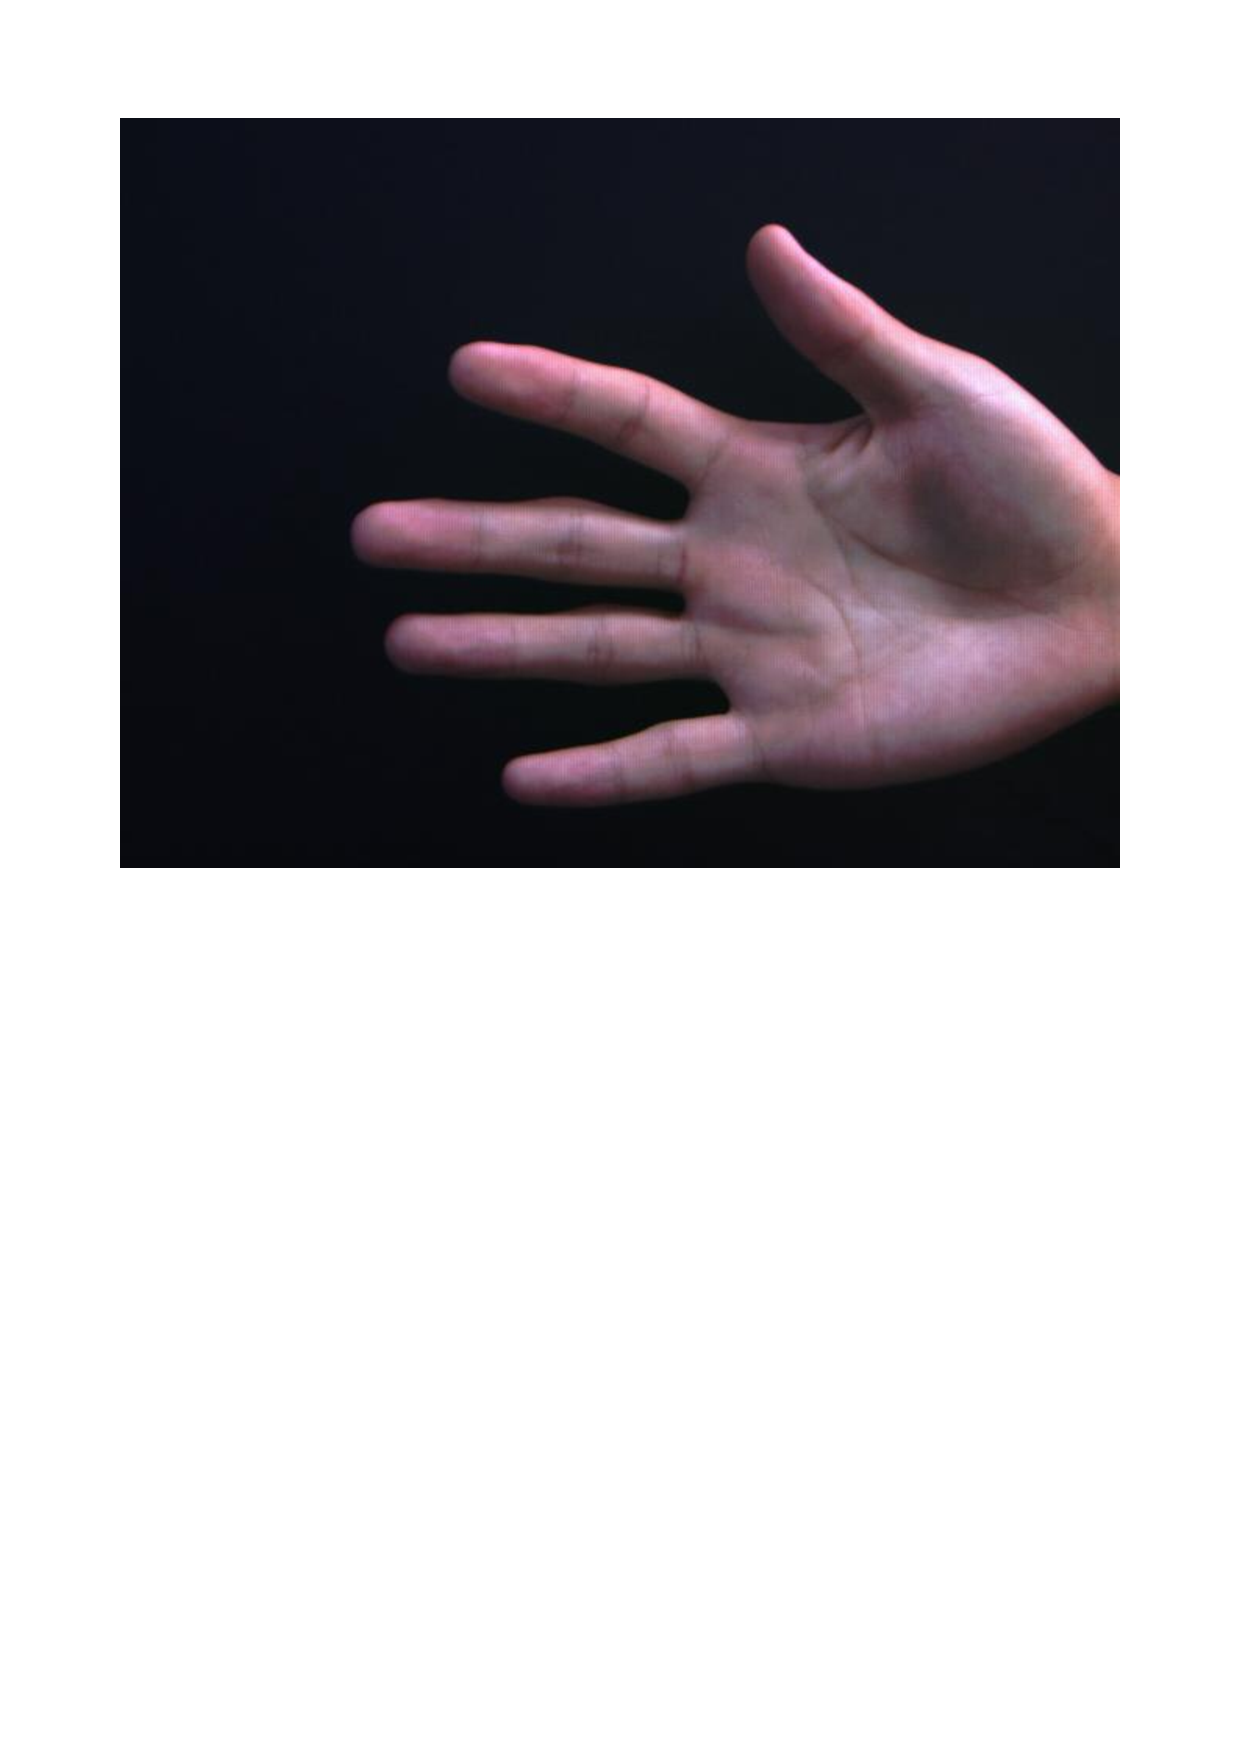
\includegraphics[page=1,scale=.57,trim=1cm 14.7cm 1cm 1.5cm,clip]{PolyU3D2D_samples.pdf}
		    \caption{\hl{Example of a hand image from the PolyU3D2D database}}
		    \label{fig:PolyU_hand1}
		\end{figure}
		\begin{figure}[!h]
		    \centering
		    \includegraphics[page=2,scale=.57,trim=1cm 14.7cm 1cm 1.5cm,clip]{PolyU3D2D_samples.pdf}
		    \caption{\hl{Example of a hand image from the PolyU3D2D database for the same subject as in Fig.} \ref{fig:PolyU_hand1} \hl{with a translation of approximately 0.2cm to the left}}
		    \label{fig:PolyU_hand2}
		\end{figure}
		\begin{figure}[!h]
		    \centering
		    \includegraphics[page=3,scale=.57,trim=1cm 14.7cm 1cm 1.5cm,clip]{PolyU3D2D_samples.pdf}
		    \caption{\hl{Example of a hand image from the PolyU3D2D database for the same subject as in Fig.} \ref{fig:PolyU_hand1} \hl{with a translation of approximately 1cm to the left}}
		    \label{fig:PolyU_hand3}
		\end{figure}
		\begin{figure}[!h]
		    \centering
		    \includegraphics[page=4,scale=.57,trim=1cm 14.7cm 1cm 1.5cm,clip]{PolyU3D2D_samples.pdf}
		    \caption{\hl{Example of a hand image from the PolyU3D2D database for the same subject as in Fig.} \ref{fig:PolyU_hand1} \hl{with a translation of approximately 1.75cm to the left}}
		    \label{fig:PolyU_hand4}
		\end{figure}

	It is worth mentioning that a second version of this database named The Hong Kong Polytechnic University Contact-free 3D/2D Hand Images Database (Version 2.0), simply denoted PolyU3D2DV2, is available. This version considers the different poses of the hands. It can be investigated that no publication considered this database in the case of FT characteristic.
	
\subsection{IIT Delhi Touchless Palmprint Database (Version 1.0)} 
	The IIT Delhi (IIT Delhi) Touchless Palmprint Database (Version 1.0) database has basically been established to overcome the variation of the hand location drawbacks of other palmprint databases, where restricted environments were designed to acquire palmprint hand images with fixed poses determined by pegs. It can be claimed that using the pegs to capture a hand image is very uncomfortable as the users are obliged to put their hand into specific location. The Biometric Research Laboratory in IIT Delhi/New Delhi/India has therefore designed a peg-free environment to capture groups of hand images and utilized different variations in order to expand the researching area in terms of trustworthy palmprint recognition. It was assembled over the period July/2006 until Jun/2007 from the IIT Delhi staff and students. This database has been provided as an open access database for the research area since October 2007. A simple design was facilitated to collect the data from the participants in a contact-free manner with high variations of movements. An indoor environment has been utilized to collect hand images from 235 participants between the ages of 12 and 57 years. Both genders were present in their hand images. An open camera was used to view the hand image before the capturing operation. The camera lens was surrounded by fluorescent lighting in a circular shape. A bitmap format is used to store the hand images \cite{IIT-Delhi-PalmprintV1}. The IIT Delhi database can be considered as high resolution coloured data, where each hand image has the size ($1200\times 1600\times 3$ pixels). The IIT Delhi Database consists of right and left images. Just the right images have been focused in FT studies.  
		\begin{figure}[!h]
		    \centering
		    \includegraphics[page=2,scale=.57,trim=1cm 14.7cm 1cm 1.7cm,clip]{IIT_samples.pdf}
		    \caption{\hl{Example of a hand image from the IIT Delhi database}}
		    \label{fig:IIT_hand1}
		\end{figure}
		\begin{figure}[!h]
		    \centering
		    \includegraphics[page=3,scale=.57,trim=1cm 14.7cm 1cm 1.7cm,clip]{IIT_samples.pdf}
		    \caption{\hl{Example of a hand image from the IIT Delhi database for the same subject as in Fig.} \ref{fig:IIT_hand1} \hl{with a rotation of approximately $10^{\circ}$ to the left}}
		    \label{fig:IIT_hand2}
		\end{figure}
		\begin{figure}[!h]
		    \centering
		    \includegraphics[page=4,scale=.57,trim=1cm 14.7cm 1cm 1.7cm,clip]{IIT_samples.pdf}
		    \caption{\hl{Example of a hand image from the IIT Delhi database for the same subject as in Fig.} \ref{fig:IIT_hand1} \hl{with a rotation of approximately $20^{\circ}$ to the right}}
		    \label{fig:IIT_hand3}
		\end{figure}
		\begin{figure}[!h]
		    \centering
		    \includegraphics[page=6,scale=.57,trim=1cm 14.7cm 1cm 1.7cm,clip]{IIT_samples.pdf}
		    \caption{\hl{Example of a hand image from the IIT Delhi database for the same subject as in Fig.} \ref{fig:IIT_hand1} \hl{with a rotation of approximately $30^{\circ}$ to the right}}
		    \label{fig:IIT_hand4}
		\end{figure}
		\begin{figure}[!h]
			\centering
			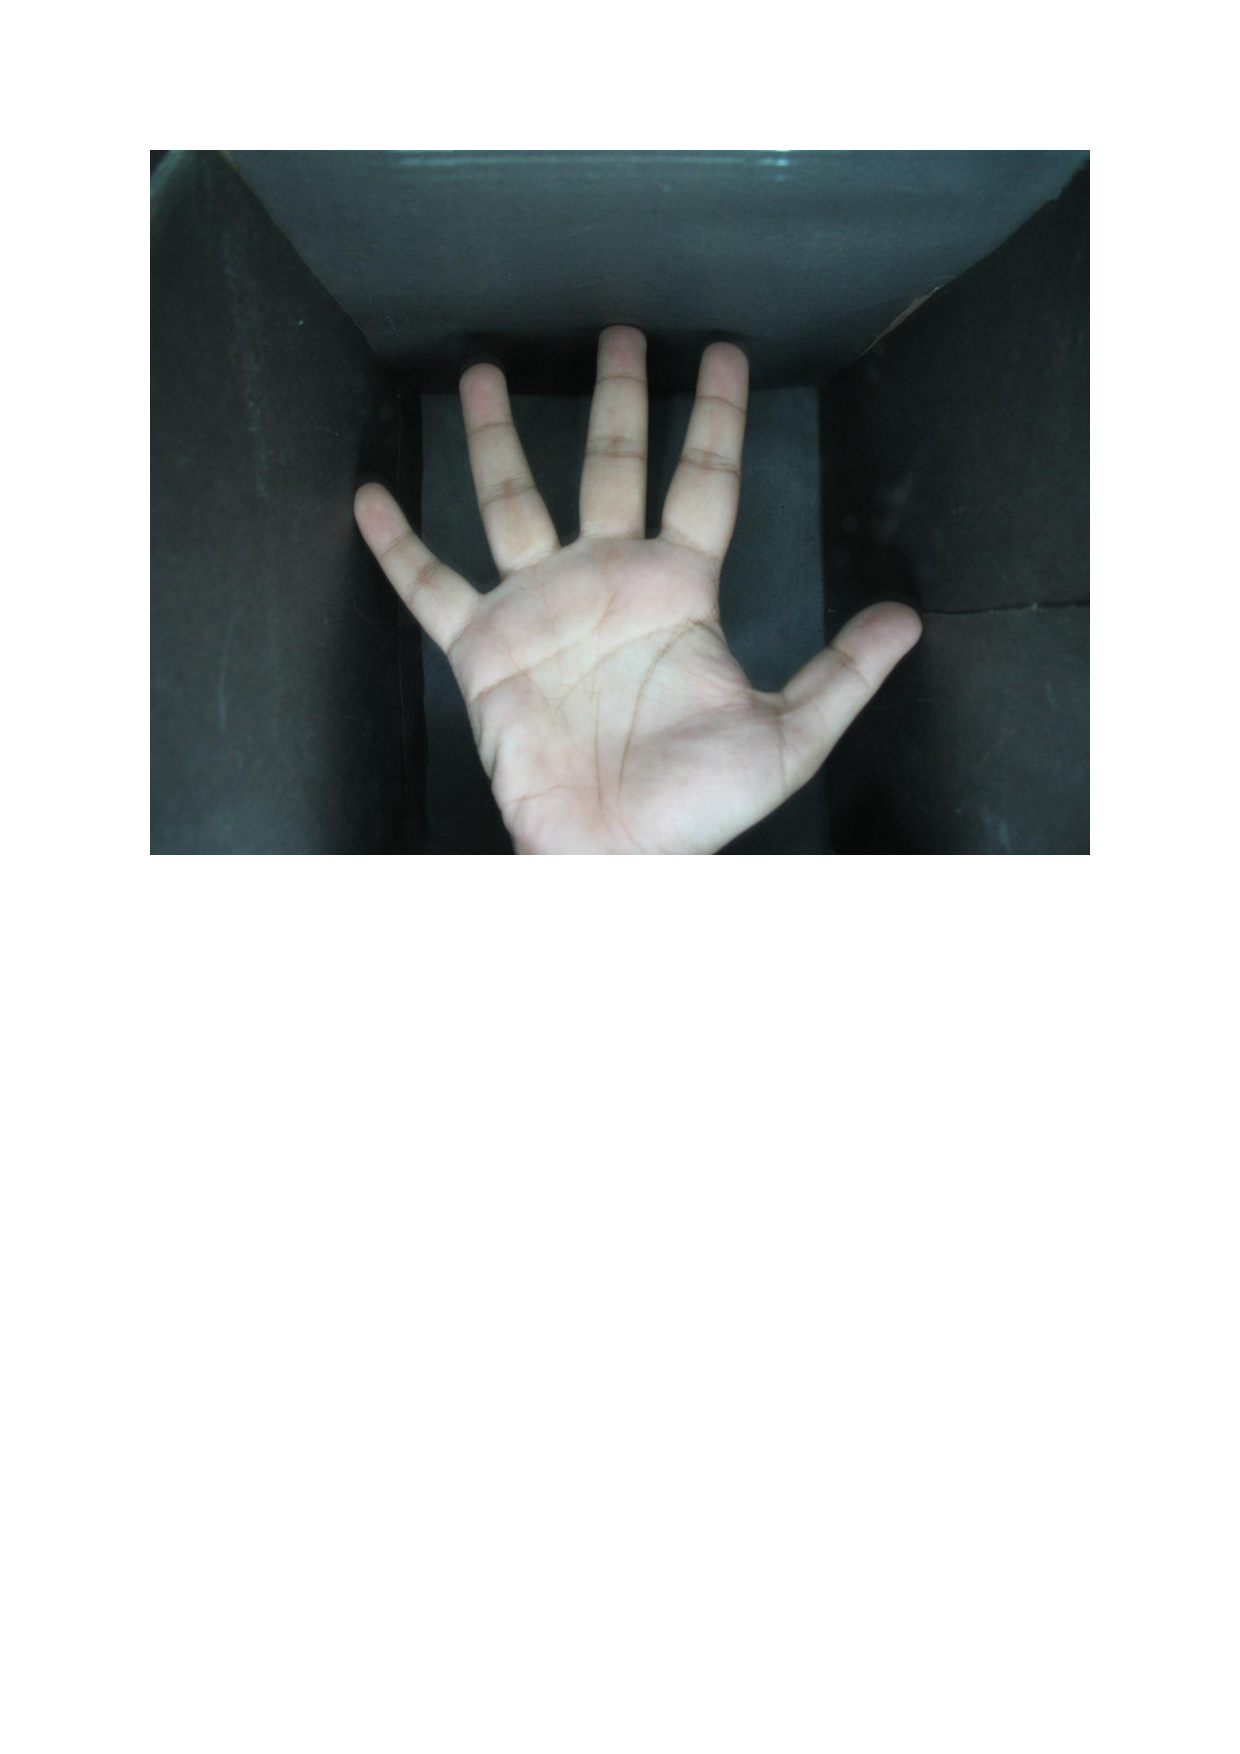
\includegraphics[page=1,scale=.57,trim=1cm 14.7cm 1cm 1.7cm,clip]{IIT_problematic.pdf}
			\caption{\hl{Sample of a hand image from the IIT Delhi database showing a middle finger bent to the back because of restricted space}}
			\label{fig:IIT_problematic_hand1}
		\end{figure}
		\begin{figure}[!h]
			\centering
			\includegraphics[page=3,scale=.57,trim=1cm 14.7cm 1cm 1.7cm,clip]{IIT_problematic.pdf}
			\caption{\hl{Sample of a hand image from the IIT Delhi database illustrating a middle finger more significantly bent to the back because of restricted space}}
			\label{fig:IIT_problematic_hand2}
		\end{figure}
		\begin{figure}[!h]
			\centering
			\includegraphics[page=2,scale=.57,trim=1cm 14.7cm 1cm 1.7cm,clip]{IIT_problematic.pdf}
			\caption{\hl{Sample of a larger hand image from the IIT Delhi database demonstrating a middle finger bent to the back because of restricted space}}
			\label{fig:IIT_problematic_hand3}
		\end{figure}
		\begin{figure}[!h]
			\centering
			\includegraphics[page=5,scale=.57,trim=1cm 14.7cm 1cm 1.7cm,clip]{IIT_problematic.pdf}
			\caption{\hl{Sample of a large hand image from the IIT Delhi database with bent middle, index and ring fingers to the back}}
			\label{fig:IIT_problematic_hand4}
		\end{figure}
		\begin{figure}[!h]
			\centering
			\includegraphics[page=6,scale=.57,trim=1cm 14.7cm 1cm 1.7cm,clip]{IIT_problematic.pdf}
			\caption{\hl{Sample of a hand image from the IIT Delhi database with a bent thumb and a rotated hand of approximately $25^{\circ}$ to the right direction, where a small amount of texture from the thumb has been lost}}
			\label{fig:IIT_problematic_hand5}
		\end{figure}
		\begin{figure}[!h]
			\centering
			\includegraphics[page=7,scale=.57,trim=1cm 14.7cm 1cm 1.7cm,clip]{IIT_problematic.pdf}
			\caption{\hl{Sample of a hand image from the IIT Delhi database illustrating a distorted hand image because of instability during the capturing operation}}
			\label{fig:IIT_problematic_hand6}
		\end{figure}
		\begin{figure}[!h]
			\centering
			\includegraphics[page=9,scale=.57,trim=1cm 14.7cm 1cm 1.7cm,clip]{IIT_problematic.pdf}
			\caption{\hl{Example of a hand image from the IIT Delhi database showing a gold ring appearing in the ring finger}}
			\label{fig:IIT_problematic_rings1}
		\end{figure}
		\begin{figure}[!h]
			\centering
			\includegraphics[page=10,scale=.57,trim=1cm 14.7cm 1cm 1.7cm,clip]{IIT_problematic.pdf}
			\caption{\hl{Example of a hand image from the IIT Delhi database demonstrating a silver ring in the middle finger}}
			\label{fig:IIT_problematic_rings2}
		\end{figure}
		\begin{figure}[!h]
			\centering
			\includegraphics[page=11,scale=.57,trim=1cm 14.7cm 1cm 1.7cm,clip]{IIT_problematic.pdf}
			\caption{\hl{Example of a hand image from the IIT Delhi database with gold and silver rings on the ring and middle fingers}}
			\label{fig:IIT_problematic_rings3}
		\end{figure}
		\begin{figure}[!h]
			\centering
			\includegraphics[page=12,scale=.57,trim=1cm 14.7cm 1cm 1.7cm,clip]{IIT_problematic.pdf}
			\caption{\hl{Example of a hand image from the IIT Delhi database showing two gold rings appearing on the ring and middle fingers}}
			\label{fig:IIT_problematic_rings4}
		\end{figure}

	This database can be considered as the most challenging one in terms of the FT studying area, because it includes hand images with various postures according to \cite{kumar2008incorporating,kumar2011personal}. 	
	\hl{Fig.} \ref{fig:IIT_problematic_hand1} \hl{shows a hand image sample with abnormal situation (a bending finger because of the restricted space).
	Figs.} \ref{fig:IIT_problematic_hand1}, \ref{fig:IIT_problematic_hand2}, \ref{fig:IIT_problematic_hand3}, \ref{fig:IIT_problematic_hand4}, \ref{fig:IIT_problematic_hand5} \hl{and} \ref{fig:IIT_problematic_hand6} \hl{show hand image samples with abnormal situations such as bending finger(s) because of restricted space and distorted hand image.}
	
	Moreover, ring jewellery can be found on one or two fingers of hand images in this database which, as mentioned, has been generated basically for palmprints. Nevertheless, these exist in all samples of the corresponding participants. In other words, they appear as parts of the FT for the participant who wear the ring(s). 
	\hl{Example of a hand image where gold and silver rings exist can be found in Fig.} \ref{fig:IIT_problematic_rings3}. 
	It is expected that the presence of the gold and silver rings in this database may affect the personal recognition performance when using the FTs as a biometric, thereby representing a useful user case.
	\hl{Examples of hand images where gold or silver rings exist can be found in Figs.}     \ref{fig:IIT_problematic_rings1}, \ref{fig:IIT_problematic_rings2}, \ref{fig:IIT_problematic_rings3} \hl{and} \ref{fig:IIT_problematic_rings4}. It is expected that their presence may affect the personal recognition performance when using the FTs as a biometric, thereby representing a useful user case.

\subsection{CASIA Multi-Spectral Palmprint Image Database (Version 1.0)} 
		\begin{figure}[!b]
			\centering
			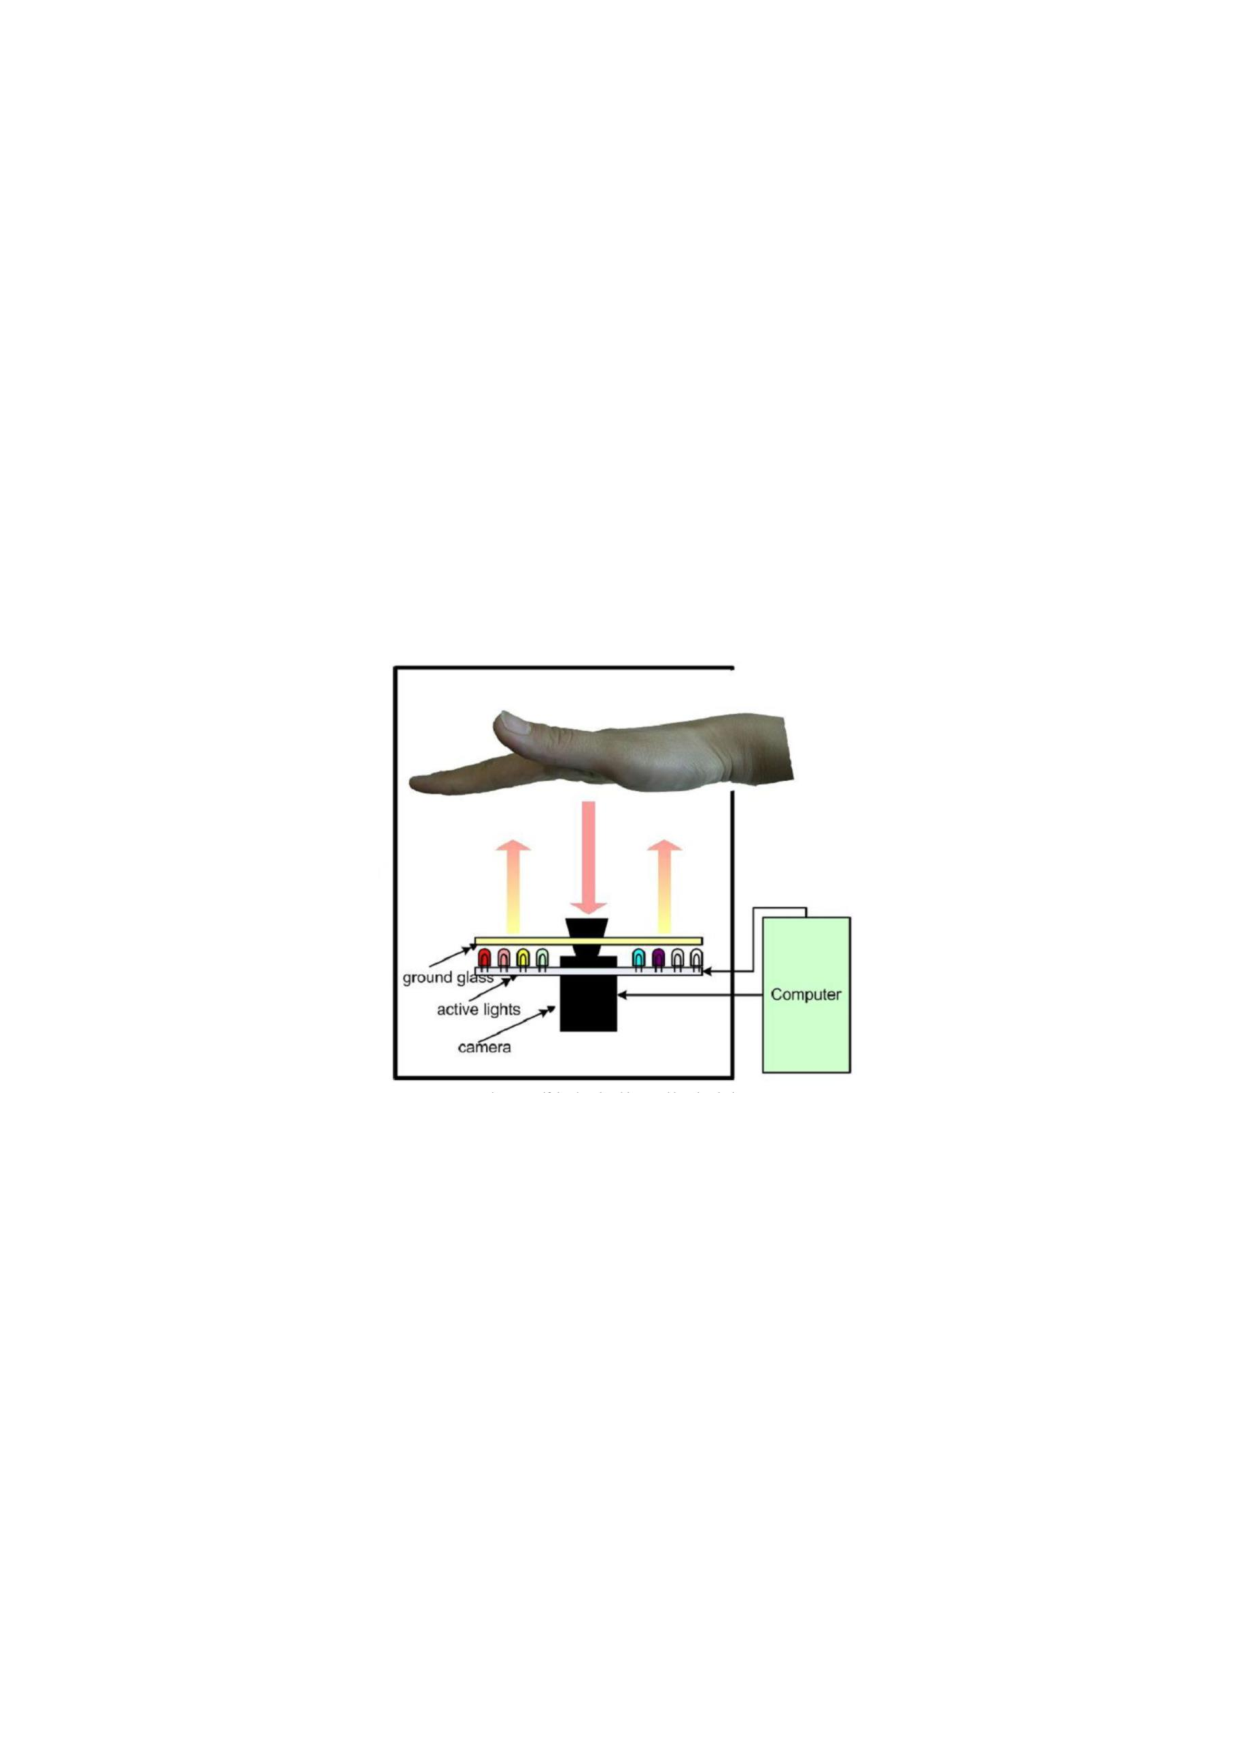
\includegraphics[page=1,scale=1.4,trim=6cm 11.1cm 6cm 10.8cm,clip]{CASIA_acquisition.pdf}
			\caption{\hl{A demonstration of the multi-spectral hand image acquisition device for the CASIAMS database as given in} \cite{CASIAMS-PalmprintV1}}
			\label{fig:CASIA_acquisition}
		\end{figure}
	In the CASIA Multi-Spectral (CASIAMS) Palmprint Image Database (Version 1.0) database, multi-spectral lights were used to acquire various features of hand images. Fundamentally, the inner skin surface of a hand shows different features when different light spectra are used. This is because of the penetration of the given spectrum. Therefore, identifiable features can be noticed under the inner skin surface of the hand after using a specific spectrum of lighting such as the veins. A multi-spectrum acquisition device was created to capture six types of patterns as hand images\hl{, see Fig.} \ref{fig:CASIA_acquisition}. 
	These images have been made open access to expand the studies of biometrics. 

	\begin{figure}[!t]
		\centering
		\includegraphics[page=1,scale=.57,trim=1cm 14.7cm 1cm 1.7cm,clip]{CASIA_multi_spectral_samples.pdf}
		\caption{\hl{Sample of a right hand image from the CASIAMS database for the wavelength lighting 460nm, where the outer texture of the skin is clarified}}
		\label{fig:CASIA_460nm_lighting}
	\end{figure}
		\begin{figure}[!h]
		    \centering
		    \includegraphics[page=2,scale=.57,trim=1cm 14.7cm 1cm 1.7cm,clip]{CASIA_multi_spectral_samples.pdf}
		    \caption{\hl{Sample of a right hand image from the CASIAMS database for the wavelength lighting 630nm, where the inner veins and outer texture of the skin are shown}}
		    \label{fig:IIT_problematic_rings2}
		\end{figure}
		\begin{figure}[!h]
		    \centering
		    \includegraphics[page=3,scale=.57,trim=1cm 14.7cm 1cm 1.7cm,clip]{CASIA_multi_spectral_samples.pdf}
		    \caption{\hl{Sample of a right hand image from the CASIAMS database for the wavelength lighting 700nm, where the inner veins and outer texture of the skin are shown}}
		    \label{fig:IIT_problematic_rings3}
		\end{figure}
		\begin{figure}[!h]
		    \centering
		    \includegraphics[page=4,scale=.57,trim=1cm 14.7cm 1cm 1.7cm,clip]{CASIA_multi_spectral_samples.pdf}
		    \caption{\hl{Sample of a right hand image from the CASIAMS database for the wavelength lighting 850nm, where the inner veins of the skin are demonstrated}}
		    \label{fig:IIT_problematic_rings4}
		\end{figure}
		\begin{figure}[!h]
		    \centering
		    \includegraphics[page=5,scale=.57,trim=1cm 14.7cm 1cm 1.7cm,clip]{CASIA_multi_spectral_samples.pdf}
		    \caption{\hl{Sample of a right hand image from the CASIAMS database for the wavelength lighting 940nm, where the inner veins of the skin are demonstrated}}
		    \label{fig:IIT_problematic_rings5}
		\end{figure}
	\begin{figure}[!h]
		\centering
		\includegraphics[page=6,scale=.57,trim=1cm 14.7cm 1cm 1.7cm,clip]{CASIA_multi_spectral_samples.pdf}
		\caption{\hl{Sample of a right hand image from the CASIAMS database for the white lighting, where the outer texture of the skin is clarified}}
		\label{fig:CASIA_white_lighting}
	\end{figure}

	The participants hand is free to move in the acquisition device. It is peg-free as there are no limitations to the location of the hand. However, the participants were expected to open their hands inside the acquisition box. A dark background (mainly black) was used. A Charge Coupled Device (CCD) camera was located at the bottom of the device and the lighting was equally distributed. A controller circuit was created to automatically activate the spectrum lighting. The specific ID of the individual was given as the name of each image file, where useful information is understandable from these names. Six images from left and right hands of 100 participants were acquired in two sessions. That is, 3 samples in session one and after more than a month additional 3 samples were collected in session two. Multi-spectral lights, which were produced by the designed sensors, were utilized to acquire 6 different image patterns at one assigned time. The applied lights had the wavelengths of 460nm, 630nm, 700nm, 850nm and 940nm. In addition to the white illumination. So, the total number of the provided CASIAMS images in this database was 7,200 right and left hand images. These were stored as Joint Photographic Experts Group (JPEG) images and they all are 8-bit grayscale. In the case of resolution, these touchless hand images can be considered as low resolution as each hand image has the size $576 \times 768$ pixels. The participants had been permitted to make determined hand movements to raise the reliability of the palmprint characteristic studies, which utilized this database. 
	\hl{Samples of the two multi-spectral hand images belonging to the same person or subject are shown in Figs.} \ref{fig:CASIA_460nm_lighting} \hl{and} \ref{fig:CASIA_white_lighting}\hl{, where each figure represents a hand image acquired by applying a specific spectrum of light} \cite{CASIAMS-PalmprintV1}. 
	\hl{Samples of the six multi-spectral hand images belonging to the same person or subject are shown in Figs.} \ref{fig:IIT_problematic_rings1}, \ref{fig:IIT_problematic_rings2}, \ref{fig:IIT_problematic_rings3}, \ref{fig:IIT_problematic_rings4}, \ref{fig:IIT_problematic_rings5} \hl{and} \ref{fig:IIT_problematic_rings6}\hl{, where each figure represents a hand image acquired by applying a specific spectrum of light} \cite{CASIAMS-PalmprintV1}. 

	In the FT studies, right hand images of Spectral 460 from the CASIAMS database were employed in \cite{Al-Nima2017Robust,Al-Nima2017efficient,Al-Nima2017finger}, because the spectrum wavelength 460nm contains FTs as cited in \cite{Khan2011Contour,khan2014multispectral}. Furthermore, it is a good opportunity to study the specifications of the FTs under a spectral light. The wavelength 460nm represents a  visible blue spectrum, where its wavelength value is between 492nm$-$455nm and this range is for the blue colour spectrum \cite{band2006light}. %as given in Table \ref{table:wavelength_frequency_spectrum}  
	
	%	\begin{table}[!h]
	%		\caption{The wavelengths and frequencies of the visible spectrum colours}
	%		\label{table:wavelength_frequency_spectrum}
	%		\centering
	%		\begin{tabular}{l|l|l}
	%			\hline\hline
	%			\textbf{Colour} & \textbf{Wavelength (nm)} & \textbf{Frequency ($10^{12}$ Hz)} \\ \hline
	%			Violet & $455-390$ & $659-769$ \\ \hline
	%			Blue & $492-455$ & $610-659$ \\ \hline
	%			Green & $577-492$ & $520-610$ \\ \hline
	%			Yellow & $597-577$ & $503-520$ \\ \hline
	%			Orange & $622-597$ & $482-503$ \\ \hline
	%			Red & $780-622$ & $384-482$ \\ \hline
	%		\end{tabular}
	%	\end{table}
	
	%	Table \ref{table:wavelength_frequency_spectrum} shows the offer wavelength of the multi-spectral lighting types. The applied lights: 630nm and 700nm belong to the red spectrum; 850nm and 900nm are included in the near infra-red spectrum; and the white is the visible white light that combines all the visible spectrum colours. 

\subsection{The Hong Kong Polytechnic University Finger Image Database (Version 1.0)}
		\begin{figure}[!b]
			\centering
			\includegraphics[page=1,scale=1,trim=5cm 11.2cm 5cm 11cm,clip]{fv_ft_device.pdf}
			\caption{\hl{Representation of the FV and FT image capturing device} \cite{Kumar2012Human}}
			\label{fig:fv_ft_device}
		\end{figure}
	The Hong Kong Polytechnic University Finger Image (PolyUFI) database (Version 1.0) is probably the first database that considers the FTs of fingers. However, the principle idea beyond establishing this database is to collect a wide range of Finger Veins (FV) images. An capturing device to collect both the FT and FV images was designed. 
	\hl{The architecture of this device is illustrated in Fig.} \ref{fig:fv_ft_device}. 
	This image capturing device was used in the campus of The Hong Kong Polytechnic University to accumulate the finger images. The time period of acquiring the data was generally between April-2009 to March-2010. Both genders male and female, were considered in this project, and 156 people provided their finger images. Each image is of a bitmap type and the total number of finger images was 6264. The ages of the participants were under 30 years, which were appropriately 93\% of overall subjects. Two sessions were organized to simultaneously capture the FV and FT images with an average interval equal 66.8 days (minimum one month and maximum more than six months). Twelve images were acquired in each session (6 images for the FV and 6 images for the FTs) from only the index and middle fingers respectively. So, 24 images were acquired for both fingers in each session. The left hands were only used in this database. \hl{Samples of FT are given in Fig.} \ref{fig:ft_images} \cite{PolyUFinTexVei}.
		\begin{figure}[!h]
			\centering
			\includegraphics[page=1,scale=.57,trim=6cm 9.5cm 6cm 8cm,clip]{ft_fv_images.pdf}
			\caption{\hl{Samples of FT images from the PolyUFI. Each FT image belongs to a subject}}
			\label{fig:ft_images}
		\end{figure}

	Many drawbacks can be investigated in this database. First of all, it contains very small regions of FTs. Secondly, just two fingers were employed in this database. Thirdly, part of fingerprints are captured together with a small part of FTs. Fourthly, just the upper knuckles are fully presented. Fifthly, as mentioned this database was established fundamentally for FV and in \cite{Kumar2012Human}, where the database was reported, a fusion method has been mainly exploited depending on the vein patterns. 
	\hl{Therefore, a comprehensive study cannot be established for the FTs by using this database.} \\
		\begin{figure}[!h]
			\centering
			\includegraphics[page=2,scale=.57,trim=3.7cm 8cm 3.7cm 8.5cm,clip]{ft_fv_images.pdf}
			\caption{\hl{Samples of FV images from the PolyUFI. Each FV image belongs to a corresponding subject to FT image in the previous figure}}
			\label{fig:fv_images}
		\end{figure}

\subsection{The Hong Kong Polytechnic University Low Resolution Fingerprint Database (Version 1.0)}
\label{subsec:PolyULRF}
	The Hong Kong Polytechnic University Low Resolution Fingerprint (PolyULRF) Database (Version 1.0) database is a subset of the PolyUFI database. So, they have been collected during the time period of April 2009 - March 2010. The elapsed time between the two acquiring sessions can be averaged to an interval of 66.8 days. The minimum interval was one month, whereas, the maximum interval was six months. This database have been collected by 156 participations of both genders (female and male). The ages of the participants are varies. However, 93\% of the users were younger than 30 years. All the images were captured in bitmaps format by using an inexpensive webcam. It composes of images that contain fingerpringts with small part of FTs for only the index finger. Each person provided 12 images acquired in two sessions (6 images in each session). Overall images in this database are 1466. The essential idea of establishing this database is to provide low resolution fingerprints for the researchers \cite{PolyULRF}. 
	\hl{Samples of PolyULRF images are given in Fig.} \ref{fig:PolyULRF}.
	
	Again, only small parts of index finger images were collected, so, one can argue that this is not sufficient to represent a comprehensive study or obtain best performance.
		\begin{figure}[!h]
			\centering
			\includegraphics[page=1,scale=.47,trim=2cm 4cm 2cm 4cm,clip]{PolyULRF.pdf}
			\caption{\hl{Samples of PolyULRF images. Each row shows different captured images for different subjects and each column shows different captured images for a same subject}}
			\label{fig:PolyULRF}
		\end{figure}
\subsection{IIITD Smartphone Fingerphoto Database}
		\begin{figure}[t]
			\centering
			\includegraphics[page=2,scale=.65,trim=2cm 15cm 2cm 2cm,clip]{IIITD_dataset.pdf}
			\caption{\hl{Examples of the natural indoor images from the IIITD database}}
			\label{fig:IIITD_Natural_Indoor}
		\end{figure}
		\begin{figure}[!h]
			\centering
			\includegraphics[page=3,scale=.65,trim=2cm 15cm 2cm 2cm,clip]{IIITD_dataset.pdf}
			\caption{\hl{Examples of the natural outdoor images from the IIITD database}}
			\label{fig:IIITD_Natural_Outdoor}
		\end{figure}
		\begin{figure}[!h]
			\centering
			\includegraphics[page=4,scale=.65,trim=2cm 15cm 2cm 2cm,clip]{IIITD_dataset.pdf}
			\caption{\hl{Examples of the white indoor images from the IIITD database}}
			\label{fig:IIITD_White_Indoor}
		\end{figure}
		\begin{figure}[!h]
			\centering
			\includegraphics[page=5,scale=.65,trim=2cm 15cm 2cm 2cm,clip]{IIITD_dataset.pdf}
			\caption{\hl{Examples of the white outdoor images from the IIITD database}}
			\label{fig:IIITD_White_Outdoor}
		\end{figure}
		\begin{figure}[!h]
			\centering
			\includegraphics[page=1,scale=.7,trim=2cm 17.5cm 2cm 2cm,clip]{IIITD_dataset.pdf}
			\caption{\hl{Examples of the live scan images from the IIITD database}}
			\label{fig:IIITD_fingerprint}
		\end{figure}

	The IIITD Smartphone Fingerphoto database, or simply IIITD database, was established for the Fingerphoto images, which acquired by using a smartphone camera. A smartphone type Apple iPhone5 with 8 Mega Pixels was employed to capture the Fingerphoto images. The auto-focus was turned on, whereas, the flash camera was turned off at the capturing time. Various background and illumination environments were used for the acquired finger images. That is, for a white background two groups of images were captured: indoor group and outdoor group. The illumination of the indoor group images was controlled, whilst, the illumination of the outdoor group images was uncontrolled. Number of people were 64 subjects, 8 images were collected to middle and index fingers of right hands. So, 2048 images were produced from (2 fingers $\times$ 8 instances $\times$ 2 light variations $\times$ 64 subjects). Similarly, 2048 images were collected by considering the same calculations, but this time for natural backgrounds. Again, two groups were considered: controlled illumination for indoor environments and uncontrolled illumination for outdoor environments. Any natural background was allowed to be captured in these two groups of images \cite{sankaran2015Onsmartphone}.
	\begin{table}[p]
		\centering
		\caption{Comparisons between the specifications of the employed databases in FT studies}
		\label{Table:Databases}
		\scalebox{0.8}{\begin{tabular}{|C{1.7cm}|C{1.7cm}|C{1.7cm}|C{1.7cm}|C{2cm}|C{2cm}|C{1.7cm}|}
			\hline
			\textbf{Database} & \textbf{PolyU3D2D} & \textbf{IIT Delhi} & \textbf{CASIAMS} & \textbf{PolyUFI} & \textbf{PolyULRF} & \textbf{IIITD} \\ \hline
			\textbf{Translations} 	 & Small variations & Big variations & Small variations & No variations & No variations & No variations \\ \hline
			\textbf{Orientations} & Small variations & Big variations & Small variations & No variations & No variations & No variations \\ \hline
			\textbf{Background environment} & Black background & Dark box & Black background & White diffusion background & White diffusion background & Varying\\ \hline
			\textbf{Illumination} & Indoor lighting & Fluorescent lighting & Wavelength 460nm & Light-emitting diodes (wavelength 850nm) & Light-emitting diodes (wavelength 850nm) & Varying \\ \hline
			\textbf{No. of people} 	 & 177 & 235 & 100 & 156 & 156 & 64 \\ \hline
			\textbf{No. of fingers (per sample)} 	 & 5 & 5 & 5 & 2 (index and middle) & 1 (index) & 2 (index and middle) \\\hline
			\textbf{Hand sided} 	 & Right & Right and left & Right and left & Left & Left & Right \\\hline
			\textbf{No. of fingers (FT parts)} 	 & 8850 & 13020 & 36000 & 3132 & 1466 & 4096 \\\hline
		\end{tabular}}
	\end{table}

	This database also includes live scan fingerprint images for online banking applications. So, a gallery was established for this group of images. A Lumidigm Venus IP65 Shell fingerprint sensor was used to acquire the fingerprint images. The key idea of establishing this gallery is to be used for the matching with fingerphoto images after obtaining their fingerprints. In this case, 1024 images were captured for (2 fingers $\times$ 8 instances $\times$ 64 subjects) \cite{sankaran2015Onsmartphone}. 
	\hl{Examples of various IIITD image types are shown in Figs.} \ref{fig:IIITD_Natural_Indoor}, \ref{fig:IIITD_Natural_Outdoor}, \ref{fig:IIITD_White_Indoor}, \ref{fig:IIITD_White_Outdoor} \hl{and} \ref{fig:IIITD_fingerprint}.

	Comparisons between the descriptions of the different employed databases are shown in Table \ref{Table:Databases}.
	%This database is established to overcome the lacking of multi-variations in fingerphoto images. Different backgrounds and illuminations were used during the acquisition. Total of 5100 images were captured for right index and middle fingers. Eight images were acquired for each finger and 64 people were participated. Three groups of data can be recognized in this database: fingerprint (or live-scan), varying illumination and varying background. Furthermore, indoor and outdoor environments were employed for each of the varying illumination and varying background. A Lumidigm Venus IP65 sensor was used to acquire the fingerprint (or live-scan) images. A smartphone type Apple iPhone5 with 8 Mega Pixels was employed to capture the Fingerphoto images. The auto-focus is turned on, whereas, the flash camera was turned off at the capturing time \cite{malhotra2017fingerphoto}. 
	%\begin{figure}[!h]
	%	\centering
	%	\includegraphics[page=5,scale=.8,trim=1.5cm 18.9cm 2.1cm 2cm,clip]{finphoto.pdf}
	%	\caption{IIITD Smartphone Fingerphoto Database with varying backgrounds and illuminations as demonstrated in \cite{sankaran2015Onsmartphone}}
	%	\label{fig:fingerphoto}
	%\end{figure}
\section{FT recognition performances}
	To evaluate the FT recognition performances, a number of common measurements were used. These measurements can be illustrated as follows:
	\begin{itemize}
		\item False Acceptance Rate (FAR): also known as False Match Rate (FMR) or False Positive Rate (FPR)\cite{Woods1997Generating,saugirouglu2009Intelligent}. It is the ratio between number of accepted imposters to the total number of imposters \cite{Goh2010Bi-modal}. 
		%	It can be represented by the following equation \cite{Goh2010Bi-modal}:\\
		%	\begin{equation}
		%		FAR = \frac{Number~of~Accepted~Imposters}{Total~Number~of~Imposters} \times 100\%
		%	\end{equation}\\
		\item False Rejection Rate (FRR): also known as False Non-Match Rate (FNMR) \cite{Woods1997Generating} \cite{saugirouglu2009Intelligent}. It is the ratio between the number of rejected clients to the total number of clients \cite{Goh2010Bi-modal}. 
		%	It can be represented by the following equation \cite{Goh2010Bi-modal}:\\
		%	\begin{equation}
		%		FRR = \frac{Number~of~Rejected~Clients}{Total~Number~of~Clients} \times 100\%
		%	\end{equation}\\
		\item Equal Error Rate (EER): It is the trade off point between the FAR and FRR. It is considered as an essential parameter to evaluate any biometric system rather than the FT recognition system. Basically, if the EER has a small value this means that the system is efficient and vice versa. Statistically, the EER is equivalent to a value of threshold in which the FRR = FAR \cite{meshoul2010novel}.
		\item True Positive Rate (TPR): Also known as Genuine Acceptance Rate (GAR) \cite{Woods1997Generating} \cite{saugirouglu2009Intelligent} or True Acceptance Rate (TAR) \cite{Debayan2018matching}. It is the ratio between the number of correctly classified positives to the total number of clients. Mathematically, It equals to 1-FRR. 
		\item Recognition rate \hl{(or recognition accuracy)}: It represents the recognition accuracy of a biometric system. Effectively, it determines how the system is successful in a percentage value.
		\item Receiver Operating Characteristic (ROC): It is a curve that represents the relationship between the FAR and TPR (or 1-FRR). The ROC is widely used	to report the recognition system measurements.
		\item Area Under the Curve (AUC): It is a value that shows the area under the ROC curve. In other words, it measures the occupied area by the ROC cure.
		\item Detection Error Tradeoff (DET): It is a curve that represents the relationship between the FAR and FRR.
		\item Cumulative Match Characteristics (CMC): It is a curve that represents the relationship between the recognition rate (or recognition accuracy) and cumulative rank. This curve is employed to show the identification performance \cite{Kumar2012Human}.
		\item Time: It usually represents an average time of implementing recognition operation(s) \cite{jaswal2016knuckle}. This evaluation has no standard equipments to be measures as it depends on the specifications of the used equipment parts during the operations. So, usually the specifications of the exploited recognition device is described for this measurement.
	\end{itemize}
	%It has been illustrated that reducing the FAR value will increase the security level of the system, whilst, increasing the FAR value will increase the flexibility of the system in terms of accepting input subjects \cite{maltoni2009handbook}.
	The recorded FT performances are clarified as follows: Ribaric and Fratric \cite{Ribaric2005Anonline} established the first combination system between the FTs and fingers-geometry, a scanner device was used to acquire the collected hand images. 
	%Both the identification and verification experiments were utilized in this study. 
	The best FT performances were recorded to 3.51\% for the identification and 0.26\% for the verification. After combining the FT with the geometry of fingers the EER for the identification was declined to 1.17\% and for the verification was reduced to 0.04\%. The same authors designed a combination system between the FTs and palmprint \cite{Ribaric2005ABiometric}. The EER of only the FTs was not reported. However, the overall performances was reported, where two identification experiments were executed. The early experiment attained the lowest EER of 0.58\%. The low cost fusion biometric system between the palm, hand geometry and FTs that designed by \cite{Ferrer2007Low} was achieved 0.13\% for the EER of using only the FTs. Different fusion methods were applied in the case of identification recognition. The best recognition performance after the combination of all the exploited characteristics was obtained by the decision fusion, where the FAR was equal to 0\% and the FRR was equal to 0.15\%.
	%The hand images were captured by an available scanner with a resolution of 150 dpi. 
	%A simple contour was utilized after the image binarization by using the Otsu threshold \cite{otsu1975threshold}. Then, the contour cartesian coordinates were converted to polar coordinates in order to calculate the locations of the tip and valley points of the fingers from the middle point of the hand base, where a hand was located in a specific location. Noticeably, not all patterns of the FTs were applied and a fixed location was used to acquire the hand images which did not allow free translations or orientation movements to be examined. 
	The main achievement of the \cite{ying2007identity} study was that addressing the effects of different hand poses. It could segment the palmprint and the five fingers of normally stretched hand parts (completed hand area should be included in the image). There was no benchmarked recognition values and no improvement fusion recognition rate. 
	%and failed with the others. This is due to how successfully the hand contour is established. 
	%"This paper presents and compares two hand texture based personal identification methods, which are called hand-print verification in this paper to denote the idea of utilizing whole hand skin image for recognition."
	Only one or two fingers were considered in \cite{nanni2009multi}, where low resolution images acquired by a camera were utilized. By employing both the middle and ring fingers the EER value was between 0.18\% and 0\% according to the parameters of the proposed BioHashing multi-matcher. The problem here is that the fingerprint region was included, and its features were not considered. So, it seems that a wasting area was involved with the FT.
	%"Finally, considering both middle and ring fingers allows the performance to reach a near zero EER; the multimatcher MM (BioHashing) described above obtains an EER of zero in the BEST hypothesis and an EER of 0.18 in the WORST hypotheses in the tested dataset."
	In \cite{Pavesic2009Finger-based}, the authors also used a scanner acquisition device to collect part of hand images. So, they used high resolution parts of hand images located in a limited space. As mentioned, the fingerprints were fused with limited areas of FTs for the four fingers of each subject. The best identification recognition rate was 99.98\% and the best verification EER value was 0.01\% after the fusion.

	Combinations between the FTs and palmprint were presented in \cite{Michael2010Robust}, \cite{michael2010innovative} and \cite{Goh2010Bi-modal}. In these publications, a Charge-coupled Device (CCD) camera was used to collect video streams of hand images. Different verification specifications were used, as clarified in the table. The EERs of only the FTs were reported to 4.10\%, 1.95\% and 2.99\% for \cite{Michael2010Robust}, \cite{michael2010innovative} and \cite{Goh2010Bi-modal}, respectively. These values were enhanced after the combinations to the EER values of 0.0034\% and 1.25\% for \cite{Michael2010Robust} and \cite{Goh2010Bi-modal}, respectively, and to the recognition rate of  99.84\% for \cite{michael2010innovative}.
	A framework study utilizing the FTs as a part of fusion between palmprint, hand geometry and finger surfaces from 2D and 3D hand images to enhance the contactless hand verification was applied by \cite{Kanhangad2011AUnified}. High EER value equal to 6\% was benchmarked for the FTs and this percentage was declined to 0.22\% after the fusion between all the utilized characteristics.
	%From Table \ref{table:four_five_fingers3} it is clear that using more features will increase the successful performance of the verification. 
	Kumar and Zhou \cite{kumar2011contactless} illustrated a biometric identification method by using a very small part part of the FT with a part of fingerprint. The PolyULRF database, which has been described in Subsection \ref{subsec:PolyULRF}, was exploited. The EER here reached 0.32\%. Similarly, A. Kumar and Y. Zhou \cite{Kumar2012Human} explained extensive identification work by employing the same database (PolyULRF) to combine between a very small part of the finger surface with the finger vein. The EER results of small part of FTs with parts of the fingerprints were as follows: for the index finger 0.32\%, for the Middle 0.22\% and for both the index and middle fingers 0.27\%. The best EER was obtained after the combination but by using only the middle finger, where it was equal to 0.02\%.
	The main idea of \cite{zhang2012hand} paper is to utilize the features of the middle finger and the palmprint in a Single Sample Biometrics Recognition (SSBR), where both can be acquired by using a single hand image sample. Recognition rates were used in this study instead of the EER to show the recognition performance. The number of participants were 100, each individual provided 10 images. So, total of 1000 images were used. This collected database was partitioned into 100 images, first image from each subject, to be stored in a template and 900 images to be assessed. 
	%The best identification performance was the one that achieved the highest recognition rate, whereas, the best verification performance was the one that achieved the lowest EER value. 
	In terms of identification: the recognition rate attained by using the feature level fusion for the middle finger was 98.33\%; the recognition rate achieved by utilizing the feature level fusion for the palmprint was 95.78\% and the recognition rate obtained by applying the score fusion to both the FLF, was increased to 99.56\%. In terms of verification: the EER value attained by using the feature level fusion for the middle finger was 1.09\%; the EER value achieved by utilizing the feature level fusion for the palmprint was 1.98\% and the EER value obtained by applying the score fusion to both the feature level fusions was decreased to 0.49\%. Again, wasting areas of fingerprints were considered here without extracting their specific features. In \cite{stein2013video}, the determined "outer area", where a part of the FT is included, was basically applied for the negative authentication. Principally, in the negative authentication the individual request is only tested for the recognition validity \cite{dasgupta2017negative}. So, there was no recognition performance assigned for the FT. The used database images were collected by "Galaxy Nexus" and "Nexus S" smartphones from Samsung. The tested photos were captured as: 541 and 569
	images form the "Galaxy Nexus" and "Nexus S", respectively. Also, 990 images where acquired by the "Galaxy Nexus" smartphone as videos. Overall, total of 2100 tested finger samples were considered. 
	As mentioned, Bhaskar and Veluchamy \cite{Bhaskar2014Hand} suggested a multi-modal biometric verification system based on feature fusion between the FTs and palmprints. This study used the IIT Delhi palmprint database, but did not describe the partitioning of training and testing sets. After the combination, the recognition rate attained 98.5\%.
	A verification approach was suggested in \cite{sankaran2015Onsmartphone}, where the IIITD fingerphoto database was reported. The main observation in this database is that it was collected under different illumination and background variations, white indoor/outdoor backgrounds and natural indoor/outdoor backgrounds. The database was randomly divided into 50\% images for gallery and 50\% images as probes for the test. By using the white indoor images in the gallery, natural outdoor images achieved the best EER value of 3.65\%. The problem here is that the fingerprint was employed with a part of the FT. An important FT study was introduced by \cite{Al-Nima2015Human}. In this publication, the FT region was assigned and all the FT parts were determined. It confirmed that using more FT features increase the successful performance of the verification. The EERs after adding the third or lower knuckle were better than the EERs without this important part. This issue was recorded in different feature extraction methods such as in the IFE based exponential histogram the EER percentage was reduced from 5.42\% to 4.07\% and in the IFE based bell-shaped histogram the EER value was declined from 12.66\% to 7.01\%. 
	The work in \cite{Al-Nima2016ANovel} was mainly established to produce a novel approach of generating the ROC graph from the PNN, as mentioned. Therefore, enhancing the recognition performance was not essential. A well-know feature extraction called the LBP obtained the best performance in that paper with a EER equal to 1.81\%.
	\begin{table}[!p]
		\centering\scriptsize
		\caption{Best FT performances for the presented recognition work with their specifications}
		\label{Table:FT_performances}
		\scalebox{0.63}{\begin{tabular}{|C{2cm}|C{2.3cm}|C{2.5cm}|C{2.6cm}|C{2cm}|C{2.5cm}|C{2cm}|}
			\hline
			\textbf{Reference} & \textbf{Database(s) type} & \textbf{Acquisition device} & \textbf{Number of employed subjects} & \textbf{Recognition type} & \textbf{Number of tested FTs\footnote{This table has been derived from the number of tested image samples per each participant multiplied by the number of used fingers.}} & \textbf{Best EER value (\%)} \\ \hline
			\multirow{3}{2cm}{\centering Ribaric and Fratric \cite{Ribaric2005Anonline}}	 & \multirow{3}{2cm}{\centering Collected images} & \multirow{3}{2cm}{\centering A scanner (180 dpi)} & \multirow{3}{1cm}{\centering 127} &  Identification & 684  clients / 2800 impostors & 3.51 \\ \cline{5-7}
			& & & & Verification & 684 clients / 159600 impostors & 0.26 \\ \hline
			Ribaric and Fratric \cite{Ribaric2005ABiometric} & Collected images & A scanner (180 dpi) & 237 & Identification & 855 clients / 3500 impostors & --- \\ \hline
			Ferrer \textit{et al.} \cite{Ferrer2007Low} & Collected images & A scanner (150 dpi) & 109 & Identification & 2616 clients / 282528 impostors & --- \\\hline
			
			Ying \textit{et al.} \cite{ying2007identity}   & UST (Not available) & A camera (150 dpi) & 287 & Identification & 129150 clients / 7400295 impostors & --- \\ \hline
			Nanni and Lumini \cite{nanni2009multi} & Collected images & A camera & 72 & Verification & 720 & --- \\ \hline
			\multirow{3}{2cm}{\centering Pavesic \textit{et al.} \cite{Pavesic2009Finger-based}} & \multirow{3}{2cm}{\centering Collected images} & \multirow{3}{2cm}{\centering A scanner (600 dpi)} & \multirow{3}{1cm}{\centering 184} & Identification & 3680 clients / 0 impostors & --- \\ \cline{5-7}
			& & & & Verification & 2760 clients / 253920 impostors & --- \\ \hline
			Michael \textit{et al.} \cite{Michael2010Robust} & Collected video stream & CCD web camera & 50 & Verification & 10-cross validation of 2500 & 4.10 \\ \hline
			Michael \textit{et al.} \cite{michael2010innovative} & Collected video stream  & CCD web camera & 100 & Verification & 18000 clients / 198000 imposters & 1.95 \\ \hline
			Goh \textit{et al.} \cite{Goh2010Bi-modal} & Collected video stream & CCD web camera & 125 & Verification & 22500 clients / 315000 imposters & 2.99 \\ \hline
			Zhang \textit{et al.} \cite{Zhang2010hand} & Collected images & CCD camera & 98 & Identification & 11-cross validation of 980 & --- \\ \hline
			Kanhangad \textit{et al.} \cite{Kanhangad2011AUnified} & PolyU3D2D & Minolta VIVID 910 & 177 & Verification & 3540 & 6 \\ \hline
			Kumar and Zhou \cite{kumar2011contactless} & PolyULRF & Web camera & 156 & Identification & 936 clients / 145,080 imposters & --- \\ \hline
			A. Kumar and Y. Zhou \cite{Kumar2012Human} & PolyUFI & Web camera & 156 & Identification & 936 clients / 145,080 imposters & --- \\ \hline
			\multirow{2}{2cm}{\centering Zhang \textit{et al.} \cite{zhang2012hand}} & \multirow{2}{2cm}{\centering Collected images} & \multirow{2}{2cm}{\centering A camera} & \multirow{2}{1cm}{\centering 100} & Identification & 900 & --- \\ \cline{5-7}
			&  &  &  & Verification & 900 & --- \\ \hline
			Stein \textit{et al.} \cite{stein2013video} & Collected images / videos & Smartphone camera & 37 & Verification & 2100 & --- \\ \hline
			Bhaskar and Veluchamy \cite{Bhaskar2014Hand} & IIT Delhi & A camera & Not given & Identification & Not given & --- \\ \hline
			Sankaran \textit{et al.} \cite{sankaran2015Onsmartphone} & IIITD & Smartphone camera & 128 & Verification & 2048 & --- \\ \hline
			Al-Nima \textit{et al.} \cite{Al-Nima2015Human} & PolyU3D2D & Minolta VIVID 910 & 177 & Verification & 3540 & 4.07 \\ \hline
			Al-Nima \textit{et al.} \cite{Al-Nima2016ANovel} & PolyU3D2D & Minolta VIVID 910 & 177 & Verification & 3540 & 1.81 \\ \hline
			Malhotra \textit{et al.} \cite{malhotra2017fingerphoto} & IIITD & Smartphone camera & 128 & Verification & 2048 & --- \\ \hline
			\multirow{4}{2cm}{\centering Al-Nima \textit{et al.} \cite{Al-Nima2017Robust}} & PolyU3D2D & Minolta VIVID 910 & 177 & Verification & 4425 & 0.34 \\ 	\cline{2-7}
			&  IIT Delhi & A camera & 148 & Verification & 740 & 1.35 \\ \cline{2-7}
			&  CASIAMS (Spectral 460nm) & CCD camera & 100 & Verification & 500 & 3 \\ \hline
			\multirow{4}{2cm}{\centering Al-Nima \textit{et al.} \cite{Al-Nima2017efficient}} & PolyU3D2D & Minolta VIVID 910 & 177 & Verification & 4425 & 0.68 \\ \cline{2-7}
			&  IIT Delhi & A camera & 148 & Verification & 740 & 2.03 \\ \cline{2-7}
			&  CASIAMS (Spectral 460nm) & CCD camera & 100 & Verification & 500 & 5 \\ \hline
			\multirow{3}{2cm}{\centering Al-Nima \textit{et al.} \cite{Al-Nima2017finger}} & PolyU3D2D & Minolta VIVID 910 & 177 & Verification & 4425 & 0.23 \\ \cline{2-7}
			&  CASIAMS (Spectral 460nm) & CCD camera & 100 & Verification & 500 & 2 \\ \hline
		\end{tabular}}
	\end{table}

	\begin{table}[!h]
	\centering\scriptsize
	\scalebox{0.63}{\begin{tabular}{|C{2cm}|C{2.3cm}|C{2.5cm}|C{2.6cm}|C{2cm}|C{2.5cm}|C{2cm}|}
			\hline
			\hl{Debayan \textit{et al.}} \cite{Debayan2018matching} & \hl{Collected images} & \hl{Xiaomi Redmi Note 4 smartphone} & \hl{309} & \hl{Verification} & \hl{4,944 clients / 95,172 impostor} & \hl{---} \\ \hline
			\hl{MAC \textit{et al.}} \cite{MAC2018contactless} & \hl{Collected video frames} & \hl{24 Megapixel digital camera} & \hl{41} & \hl{Verification} & \hl{10-fold cross validation} & \hl{---} \\ \hline

			\hl{MAC \textit{et al.}} \cite{Jahan2018Contactless} & \hl{Collected video frames} & \hl{24 Megapixel digital camera} & \hl{41} & \hl{Verification} & \hl{10-fold cross validation} & \hl{---} \\ \hline
			
			\hl{Wasnik \textit{et al.}} \cite{Wasnik2018Improved} & \hl{Collected video frames} & \hl{iPhone 6s} & \hl{48} & \hl{Verification} & \hl{240} & \hl{---} \\ \hline
			
			\hl{Wasnik \textit{et al.}} \cite{wasnik2018baseline} & \hl{Collected video frames} & \hl{iPhone 6s} & \hl{48} & \hl{Verification} & \hl{240 clients / 11280 imposter } & \hl{---} \\ \hline 

			\multirow{3}{2cm}{\centering \hl{Weissenfeld \textit{et al.}} \cite{Weissenfeld2018contactless}} & \multirow{3}{2cm}{\centering \hl{Collected images}} & \hl{LG G5 850 mobile phone and Huawei P9 mobile phone} & \hl{12} & \hl{Verification} & \hl{1920 images} & \hl{---} \\ \cline{3-7}
			&   & \hl{Handheld embedded device} & \hl{94} & \hl{Verification} & \hl{Not clear} & \hl{---} \\ \hline
			\hl{Chopra \textit{et al.}} \cite{Chopra2018Unconstrained} & \hl{Different smartphones such as iPhone; Google Nexus and Samsung Galaxy} & \hl{Smartphone camera} & \hl{115} & \hl{Verification} & \hl{Not clear} & \hl{---} \\ \hline


			\multirow{6}{2cm}{\centering \hl{Omar \textit{et al.}} \cite{omar2018deep}} & \hl{PolyU3D2D} & \hl{Minolta VIVID 910} & \hl{177} & \hl{Verification} & \hl{4425} & \hl{---} \\ \cline{2-7}
			&  \hl{IIT Delhi} & \hl{A camera} & \hl{148} & \hl{Verification} & \hl{740} & \hl{---} \\ \cline{2-7}
			&  \hl{CASIAMS (Spectral 460nm)} & \hl{CCD camera} & \hl{100} & \hl{Verification} & \hl{500} & \hl{---} \\ \cline{2-7}
			&  \hl{CASIAMS (Spectral White)} & \hl{CCD camera} & \hl{100} & \hl{Verification} & \hl{500} & \hl{---} \\ \hline
			
			\multirow{3}{2cm}{\centering \hl{Al-Nima \textit{et al.}}
			\cite{al2018personal}} 			&  \hl{CASIAMS (Spectral 460nm)} & \multirow{3}{2cm}{\centering \hl{CCD camera}} & \multirow{3}{2cm}{\centering \hl{100}} & \multirow{3}{2cm}{\centering \hl{Verification}} & \multirow{3}{2cm}{\centering \hl{800}} & \multirow{3}{2cm}{\centering \hl{0}} \\ \cline{2-2}
			& \hl{CASIAMS (Spectral White)} & & & & & \\ \hline 
			\multirow{3}{2cm}{\centering \hl{Al-Kaltakchi \textit{et al.}}}&  \hl{CASIAMS (Spectral 460nm)} & \multirow{3}{2cm}{\centering \hl{CCD camera}} & \multirow{3}{2cm}{\centering \hl{100}} & \multirow{3}{2cm}{\centering \hl{Verification}} & \multirow{3}{2cm}{\centering \hl{800}} & \multirow{3}{2cm}{\centering \hl{2}} \\ \cline{2-2}
			& \hl{CASIAMS (Spectral White)} & & & & & \\ \hline 
			
			
		\end{tabular}}
	\end{table}
	The recognition specifications in \cite{malhotra2017fingerphoto} is very similar to \cite{sankaran2015Onsmartphone} as same database, result and problem were considered. Al-Nima \textit{et al.} \cite{Al-Nima2017Robust} illustrated a robust finger segmentation method, efficient feature extraction method to extract the main FT patterns and a novel salvage approach to rescue the missing FT features. It was applied for all the five fingers and attained results consistent with \cite{Al-Nima2015Human}, where by adding the FTs of the thumb the verification performances were enhanced. The best EER values for the three databases PolyU3D2D, IIT Delhi and CASIAMS (Spectral 460) were equal to 0.11\%, 1.35\% and 3\%, respectively. It is worth mentioning that the proposed salvage approach for the missing FT parts has the capability to enhance the verification performance. That is when an amputation may happen to the employed fingers, the salvage approach can be used with the PNN to reduce the risk of obtaining a wrong verification. Efficient finger segmentation approach was suggested in \cite{Al-Nima2017efficient}, where it was established for this reason. This paper exploited the LLBP as a feature extraction. This method achieved reasonable performances, due to the fact that it considers the vertical and horizontal lines in its operator and this is appropriate for the main patterns of the FTs. Since the best lengths of the LLBP vectors are (N=13, N=15, N=17 and N=19) as suggested in \cite{Petpon2009Face}, all of these lengths were considered. The best performances were obtained by the lengths N=13(and 17), N=13, and N=19 for the PolyU3D2D, IIT Delhi and CASIAMS (Spectral 460) databases, respectively. For the same order, the best EER percentages were 0.68\%, 2.03\% and 5\%, respectively.
	That FCFNN that proposed in \cite{Al-Nima2017finger} was specifically designed to fuse the FTs of fingers. This approach was inspired from the contribution of each finger. For instance, the contribution of the thumb finger is not equal to the contribution of the index or middle finger. The recognition performance was enhanced for the PolyU3D2D database from 0.68\% to 0.23\% after using the FCFNN with the MSALBP feature extraction. Also, the best EER value was 2\% for the CASIAMS (Spectral 460) database after using the PNN with the MSALBP and after using the FCFNN with the MSALBP too. In this study the effects of the amputated fingers were also considered by taking advantages from the flexible architecture of the FCFNN. \hl{Debayan \textit{et al.}} \cite{Debayan2018matching} \hl{collected fingerphoto and fingerprint images in India from 309 subjects. The fingerphoto images were obtained by using Xiaomi Redmi Note 4 smartphone. Fingerprints with small parts of FTs were considered in this study for two index fingers and two thumb fingers from each hand. Furthermore, two mobile phone applications were exploited in the case of verification. Total of 4,944 genuine scores (309
	subjects $\times$ 4 fingers $\times$ 2 enrollment impressions $\times$ 2 verification impressions) and total of 95,172 impostor scores (309 fingers $\times$ 308 fingers) were evaluated. The performances were generally reported by calculating the TAR and fixing the FAR value to 0.1\%. The TAR was equal to 72.14\% in the first application and 99.66\% in the second application for the fingerphoto-to-fingerphoto
	matching and for fusing between all four employed fingers.} \hl{MAC \textit{et al.}} \cite{MAC2018contactless} \hl{presented a verification study based on contactless multiple finger segments. Finger images acquired by 24 Megapixel digital camera from a number of video frames (around 20-40) that covers 1.5 second interval for each participant. The participants were from different nationalities and they were asked to provide various rotation and scaling movements. 1341 images were utilized 41 individuals. The authors concentrated on contactless multiple index finger segments, where three areas were segmented from the three finger knuckles. Various types of fusions based on the Concatenation rule were considered between the finger segments feature level; sensor level; and feature and sensor levels. The recognition (classification) accuracies for the three combination methods were respectively recorded as follows 95.37\%; 97.70\% and 97.93\%. Obviously, the best performance was obtained by using the feature and sensor levels fusion method. 10-fold cross validation and SVM (RBF kernel) were used to evaluate the performance.} \hl{MAC \textit{et al.}} \cite{Jahan2018Contactless} \hl{exploited the same facilities and tools of the previous work. Nonetheless, only the sensor level combination with concatenation rule was used and the recognition (classification) accuracy of  92.99\% was calculated with a negative group of 49889 samples and a positive group of 1238 samples.} 

	\hl{Wasnik \textit{et al.}} \cite{Wasnik2018Improved} \hl{constructed improved fingerphoto verification system by using a smartphone of iPhone 6s mobile phone to collect video frames of finger images (flashlight turned on). The left index finger was examined for 48 subjects; 96 videos and 240 frames. The EER value was 2.76\% for the proposed feature extraction (the multi-scale	second order Gaussian derivatives).} \hl{Wasnik \textit{et al.}} \cite{wasnik2018baseline} \hl{utilized the same tools and facilities of the previous work. The authors here compared three non-commercial applications with one mobile phone commercial application in the case of individual verification based on the fingerphoto. Comparison of 240 genuine and 11280 imposter for 48 individuals were performed. Three feature extractions were utilized as non-commercial applications: LBP; HOG and BSIF with the classifier of Probabilistic Collaborative Representation classifier (ProCRC). The EER of the employed feature extractions are 12.83\%, 15.85\% and 18.67\%, respectively. This was compared with a commercial COST and VeriFinger SDK from} \cite{NEURO_technology} \hl{as a baseline. The EER here was much better as it attained 6.05\%. Therefore, the authors recommended to add more pre-processing steps to non-commercial applications in order to overcome commercial applications.} \hl{Weissenfeld \textit{et al.}} \cite{Weissenfeld2018contactless} \hl{illustrated a human verification work in the case of in boarder control requirement. Two mobile phones types LG G5 850 and Huawei P9 were used for the evaluation. 12 individuals were participated with 4-fingers and total of 1920 images. The EER here is about 1.0\% for a single finger. It has been cited that including all the four fingers caused increasing the performance, but there were no details about such claim. Additional examinations were performed by using a suggested handheld embedded device. This devise was designed to capture face and fingerphoto images in the border between Romania and Moldavia. Only left and right index finger is employed in this part. 184 interactions with 94 individuals were performed. Just 11 wrong interactions (6\%) were happened, 1 during acquiring a fingerphoto image and 10 during recognizing face images. As mentioned, this approach is still under development.}
	\hl{Chopra \textit{et al.}} \cite{Chopra2018Unconstrained} \hl{approached fingerphoto segmentation method by employing pre-trained VGG SegNet} \cite{Badrinarayanan2017SegNet}\hl{. A smartphone camera was utilized to collect index and/or middle fingerphoto images. Different smartphones were used in this paper (up to 45 devices), such as iPhone; OnePlus; Redmi devices; Micromax	Canvas; Lenovo K4; Lenovo K3 Note; HTC devices; Google Nexus; Samsung	Galaxy; Moto G and Moto C. This added more challenging to this study because each smartphone has different camera specifications. Moreover, to add transmission compression effects to finger images, social media applications were utilized such as Facebook messenger; Telegram  and WhatsApp.
	The employed finger images could be from any hand, but the participant had to use the same finger and the same finger postures during the testing process of verification. This can be considered as the main drawback of this work. Two essential group of experiments were applied, single finger group and multiple fingers group. For 115 subjects, total of 3450 images were collected. The database was partitioned into training and testing sets (50\% each). The EER achieved 44.35\% for the CompCode with the HD method and 35.48\% for the ResNet50 with the cosine similarity method. Clearly, the performance is low. The authors due this challenging nature of the employed database.}


	\hl{Omar \textit{et al.}} \cite{omar2018deep} \hl{attained interesting results in terms of verification, where the deep learning is exploited with the FT and a novel DFTL has been approached. Four databases were employed in this study. These are PolyU3D2D; IIT Delhi; CASIAMS (Spectral 460) and CASIAMS (Spectral White), recognition accuracies of 100\%; 98.65\%; 100\% and 98\% were respectively achieved. The drawback of this work is considering any successful FT in any five fingers to confirm the verification.} \hl{Al-Nima \textit{et al.}} \cite{al2018personal} \hl{suggested two new methods. One for the feature extraction called the SPC and another for the combination named the RPNN. Two databases of FT that acquired under two different lighting from the CASIAMS is utilized in this work. These are the CASIAMS (Spectral 460) and CASIAMS (Spectral White). FTs of only the four or main fingers were applied. The EER values of using the SPC feature extraction with normal PNN} \cite{PNN_MatlabCode} \hl{were equal to 4\% and 2\% for the CASIAMS (Spectral 460) and CASIAMS (Spectral White) databases, respectively. High verification performances of EER equal to 0\% were obtained after using the novel RPNN.} \hl{Al-Kaltakchi \textit{et al.}} \cite{al2018finger} \hl{examined different fusion levels between FTs databases of the CASIAMS (Spectral 460) and CASIAMS (Spectral White). Two sets of four fingers were utilized for each person in this study too. The four	fusion levels were evaluated: sensor level; feature level; score level and decision level. Various rules were considered: average; summation; multiplication;	maximum; minimum and concatenation. Only the concatenation rule could not be used with the decision level as this is not applicable, AND and OR rules were employed instead. Best recognition performance was reported for the	feature level fusion with the concatenation rule as the EER reached its lowest value of 2\%.}

	Best EER performances of the presented FT work with their specifications are given in Table \ref{Table:FT_performances}. As it can be seen that the performances of the suggested FT recognition approaches are generally still requiring more improvements. Large numbers of FT samples can be easily acquired. Many effective ideas can be proposed to perform FT biometric systems with high levels of accuracy. Furthermore, many approaches can be adopted to enlarge the research areas of the FT recognition field. 

\section{Conclusion and Future Work}
	The findings of this survey have found a number of important observations in FT studies. Firstly, for the finger segmentation and ROI collection, the majority of the previous studies considered limited areas of the FT regions. Secondly, FT patterns lacked for a beneficial feature extraction model that can efficiently collect its ridges, visible lines and skin wrinkles features. Thirdly, usually the FTs were combined with supported biometric characteristic(s) to construct multi-modal biometric structures. Whereas, this trait can be used alone as multi-objects by considering the FT of each finger as a single object. 
	
	The employed and available FT databases were reviewed. These are as follows: the PolyU3D2D; the IIT Delhi Database and the CASIAMS (Spectral 460), PolyUFI, PolyULRF and IIITD databases. Also, essential observations have been notices. The databases which have been used are fundamentally established for palmprint or fingerprint studies. So, it is believed that a specific FT database is required, where this database has to cover the full FT regions and involve all of the feature types (wrinkles, visible lines and ridges).
	%From the previous literature, it can be observed that the FTs have been used as a part of a multi-modal biometric scheme. In addition, limited FT features have been utilized as the majority of the ROI extracting approaches collected just part of the FTs. 
	%It can be argued that reliable biometric recognition approaches can be established by exploiting the FT patterns of multiple fingers in a fused multi-object prototype. This will reduce the cost of providing an additional acquiring device and establishing an extra applicable algorithm for including another biometric trait to be combined with the FTs. \\
	%In addition, many publications completely ignored the minutiae patterns.

	Regarding the recognition performances, it can be concluded that the FTs were efficiently exploited in many recognition systems. A large number of FT samples is easy to be collected. The FTs can provide effective recognition contributions if they are exploited in single-modal or multi-modal biometric systems. Nevertheless, the recognition performance based on the FT(s) can be further improved. Also, many ideas can be adopted to increase the investigations of this field. 

	Moreover, the following insights are suggested for future work:
	\begin{itemize}
		\item \hl{Biometric application projects and systems based on the FT(s) can be produced.}
		\item There is no sufficient information for the ridge patterns of the FT, so, they require to be focused in future studies. 
		\item \hl{Ridge information of all fingers can be obtained by using smartphones just as the fingerphoto images. Android applications may be employed for this matter.}
		\item The permanency of the ridge patterns needs to be examined in order to see if they are also vanished for the elderly people like the fingreprint or not.
		\item A comprehensive database is required. It should include all the FT patterns (wrinkles, visible lines and ridges).
		\item In the case of finger segmentations, additional efforts will be required to generate a robust ground truth. The current suggested ground truth is based on the essential points of fingers (tips and valleys). Obviously, these points can not cover all the patterns of the lower knuckles. So, a justified ground truth for the finger segmentation can be established then provided to other researchers. 
		\item Injured or uncleared FT patterns are worth to be investigated in terms of recognition performances.
		\item The affects of skin diseases are also need to be considered in future studies. Some of these diseases can be overcomes by the power of image processing such as the rash. Others may influence the pattern shapes such as acnes. Nevertheless, the wide area of spreading FT patterns may help the biometric systems to stay obtaining the correct recognition.
		\item An intensive study may be established to decide which part of the FT is more effective in terms of individual recognition. 
		\item Multi-spectral sensors can be used to reveal different FT patterns. Then, fusion studies can be performed between the different extracted patterns.
		\item \hl{Hyperspectral imaging of FTs are worth studying, where interesting FT patterns and textures are revealed according to the afforded electromagnetic spectra.}
		\item A deep learning technique can be employed to extract the FT features and recognize the users, provided sufficient data are available.
		\item \hl{The terminology of Finger Inner Surface (FIS) can be used in future work as it provides the same meaning of FT.}
\end{itemize}

\section*{Acknowledgement}
	$\bullet$ "RC grant EP/P015387/1".\\
	$\bullet$ "The Hong Kong Polytechnic University  Contact-free 3D/2D Hand Images Database version 1.0". \\
	$\bullet$ "IIT Delhi Palmprint Image Database version 1.0".\\
	$\bullet$ "Portions of the research in this paper use the CASIA-MS-PalmprintV1 collected by the Chinese Academy of Sciences' Institute of Automation (CASIA) ".

% Bibliography
\bibliographystyle{ACM-Reference-Format}
\bibliography{references15}

\end{document}
